\documentclass[11pt, a4paper]{scrartcl}

% Core packages.
\usepackage[USenglish]{babel}
\usepackage[T1]{fontenc}
\usepackage[utf8]{inputenc}
\usepackage[top=1.5cm, left=1.5cm, right=1.5cm, bottom=2.5cm]{geometry}
% Math packages.
\usepackage{amssymb}
\usepackage{bbm}
\usepackage{bm}
\usepackage{cancel}
\usepackage{mathtools}
\usepackage{physics}
\usepackage{siunitx}
% Other packages.
\usepackage{csquotes}
\usepackage[hidelinks=true]{hyperref}
\usepackage{todonotes}
\usepackage{tikz}
\usepackage{xspace}
\usetikzlibrary{positioning}

% Document information.
\title{Pattern Recognition and Machine Learning}
\subtitle{Exercises}
\author{Fabian Damken}
\date{\today}

% Styling.
\MakeOuterQuote{"}
\mathtoolsset{showonlyrefs, showmanualtags}
\presetkeys{todonotes}{inline}{}

% Macros.
% Math.
\newcommand{\E}{\mathbb{E}}
\newcommand{\Var}{\mathbb{V}}
\DeclareMathOperator{\cov}{cov}
\DeclareMathOperator{\mode}{mode}
\newcommand{\KL}{D_\mathit{KL}}
\newcommand{\N}{\mathbb{N}}
\newcommand{\Z}{\mathbb{Z}}
\newcommand{\R}{\mathbb{R}}
\newcommand{\C}{\mathbb{C}}
\newcommand{\normal}{\mathcal{N}}
\newcommand{\transposed}{{\!\top\!}}
\renewcommand{\vec}[1]{\bm{#1}}
\newcommand{\mat}[1]{\bm{\mathrm{#1}}}
\newcommand{\given}{\,\vert\,}
\newcommand{\biggiven}{\,\big\vert\,}
\newcommand{\Biggiven}{\,\Big\vert\,}
\newcommand{\bigggiven}{\,\bigg\vert\,}
\newcommand{\Bigggiven}{\,\Bigg\vert\,}
\newcommand{\qed}{\hfill\(\square\)}
\newcommand{\eot}{\hfill\(\blacksquare\)}
\newcommand{\qedeot}{\hfill\(\square\blacksquare\)}
\newcommand{\liminmeansquare}{\mathop{\mathrm{l.i.m}}\displaylimits}
% Other.
\newcommand{\github}{\href{https://github.com/fdamken/gpml}{GitHub}\footnote{\url{https://github.com/fdamken/gpml}}\xspace}
\newcommand{\seegithub}{See \github.}
\newcommand{\task}[2]{\subsection*{Task #1: #2}}

\newcommand{\diffstar}{\texorpdfstring{\raisebox{-1pt}{\resizebox{!}{8pt}{\(\star\)}}}{*}}
\newcommand{\onestar}  {(\diffstar)}
\newcommand{\twostar}  {(\diffstar\,\diffstar)}
\newcommand{\threestar}{(\diffstar\,\diffstar\,\diffstar)}

\begin{document}
	\maketitle

	\begin{abstract}
		This document are my own results from working through the exercises of the book \emph{\@title} by Christopher M. Bishop. I tried to keep all notations as close to the book as possible. A \(\square\) marks the end of a proof while a \(\blacksquare\) marks the end of a task.
	\end{abstract}

	\section{Introduction}
		\subsection{Minimizing the Sum-of-Squares Error Function  \onestar}
			To find the optimal weights of the polynomial
			\begin{equation}
				y(x, \vec{w}) = \sum_{j = 0}^{M} w_j x^j  \label{eq:1-1-poly}
			\end{equation}
			with respect to the sum-of-squares error function
			\begin{equation}
				E(\vec{w}) = \frac{1}{2} \sum_{n = 1}^{N} \big( y(x_n, \vec{w}) - t_n \big)^2,  \label{eq:1-1-error}
			\end{equation}
			the derivative of the latter w.r.t. the weights \(\vec{w}\) has to be calculated. This requires the application of the chain rule. The partial derivatives of \eqref{eq:1-1-poly} are given as
			\begin{equation}
				\pdv{y(x, \vec{w})}{w_i} = \sum_{j = 0}^{M} \delta_{ij} x^j,
			\end{equation}
			where \( \delta_{ij} \) is the Kronecker delta. Combined with the partial derivative of \eqref{eq:1-1-error} w.r.t. the polynomial \eqref{eq:1-1-poly},
			\begin{equation}
				\pdv{E(\vec{w})}{y(x, \vec{w})} = \sum_{n = 1}^{N} \big( y(x_n, \vec{w}) - t_n \big),
			\end{equation}
			the whole derivative is given as
			\begin{align}
				\dv{E(\vec{w})}{w_i}
					&= \pdv{E(\vec{w})}{y(x, \vec{w})} \pdv{y(x, \vec{w})}{w_i}
					 = \sum_{n = 1}^{N} \sum_{j = 0}^{M} \delta_{ij} x^j \big( y(x_n, \vec{w}) - t_n \big)
					 = \sum_{n = 1}^{N} \sum_{j = 0}^{M} \delta_{ij} x^j \Bigg( \sum_{k = 0}^{M} w_k x_n^k - t_n \Bigg) \\
					&= \sum_{n = 1}^{N} \sum_{j = 0}^{M} \sum_{k = 0}^{M} \delta_{ij} w_k x_n^{j + k} - \sum_{n = 1}^{N} \sum_{j = 0}^{M} \delta_{ij} x_n^j t_n
					 = \sum_{n = 1}^{N} \sum_{k = 0}^{M} w_k x_n^{i + k} - \sum_{n = 1}^{N} x_n^i t_n \\
					&= \sum_{k = 0}^{M} w_k \underbrace{\sum_{n = 1}^{N} x_n^{i + k}}_{A_{ik} \,\coloneqq} - \underbrace{\sum_{n = 1}^{N} x_n^i t_n}_{T_i \,\coloneqq}
					 = \sum_{j = 0}^{M} A_{ik} w_k - T_i
			\end{align}
			Setting this quantity to zero yields exactly the linear equation system given in the task,
			\begin{equation}
				\sum_{j = 0}^{M} A_{ik} w_k = T_i,  \label{eq:1-1-linear}
			\end{equation}
			where \(A_{ik}\) and \(T_i\) are defined as in the above equation.

			\eot
		% end

		\subsection{Regularized Sum-of-Squares  \onestar}
			For the regularized error function
			\begin{equation}
				\tilde{E}(\vec{w}) = E(\vec{w}) + \frac{\lambda}{2} \lVert \vec{w} \rVert_2^2,
			\end{equation}
			the derivative is extended by the partial derivative of the regularization term,
			\begin{equation}
				\pdv{w_i} \frac{\lambda}{2} \lvert \vec{w} \rVert_2^2 = \lambda w_i.
			\end{equation}
			This yields the following derivative:
			\begin{equation}
				\dv{\tilde{E}(\vec{w})}{w_i}
					= \dv{E(\vec{w})}{\vec{w}} + \pdv{w_i} \frac{\lambda}{2} \lvert \vec{w} \rVert_2^2
					= \pdv{E(\vec{w})}{y(x, \vec{w})} \pdv{y(x, \vec{w})}{w_i} + \pdv{\lVert \vec{w} \rVert_2^2}{w_i}
					= \sum_{j = 0}^{M} A_{ik} w_k - T_i + \lambda w_i
			\end{equation}
			Analogous to \eqref{eq:1-1-linear}, the linear system of equations is given as
			\begin{equation}
				\sum_{j = 0}^{M} A_{ik} w_k = T_i - \lambda w_i
			\end{equation}
			which can be found by setting the derivative to zero. The variables \(A_{ik}\) and \(T_i\) are defined accordingly.

			\eot
		% end

		\subsection{Apples, Oranges, Limes, and Boxes  \twostar}
			Firstly, for each box \( B \in \{ r, b, g \} \), the probabilities of picking any fruit has to be calculated, i.e., the probabilities \( p(F \given B) \), where \( F \in \{ a, o, l \} \) is the random variable for the picked fruit with the possible values "apple", "orange", and "lime", respectively. The random variable \( R \) describes which fruit is removed. These probabilities depend on the box, too, and are given by the frequencies of the items in the boxes:
			\begin{center}
				\begin{tabular}{c|ccc}
					\( p(R \given B) \) & \(B = r\) & \(B = b\) & \(B = g\) \\ \hline
					     \(R = a\)      & \(3/10\)  &  \(1/2\)  & \(3/10\)  \\
					     \(R = o\)      &  \(2/5\)  &  \(1/2\)  & \(3/10\)  \\
					     \(R = l\)      & \(3/10\)  &   \(0\)   &  \(2/5\)
				\end{tabular}
			\end{center}
			The conditional probabilities \( p(F \given R, B) \) are then easy to calculate by subtracting one from the respective frequencies:
			\begin{center}
				\begin{tabular}{c|ccc}
					\( p(F \given R, B = r) \) & \(R = a\) & \(R = o\) & \(R = l\) \\ \hline
					        \(F = a\)          &  \(2/9\)  &  \(1/3\)  &  \(1/3\)  \\
					        \(F = o\)          &  \(4/9\)  &  \(1/3\)  &  \(4/9\)  \\
					        \(F = l\)          &  \(1/3\)  &  \(1/3\)  &  \(2/9\)
				\end{tabular}
				\qquad
				\begin{tabular}{c|ccc}
					\( p(F \given R, B = b) \) & \(R = a\) & \(R = o\) & \(R = l\) \\ \hline
					        \(F = a\)          &   \(0\)   &   \(1\)   &  \(1/2\)  \\
					        \(F = o\)          &   \(1\)   &   \(0\)   &  \(1/2\)  \\
					        \(F = l\)          &   \(0\)   &   \(0\)   &   \(0\)
				\end{tabular} \\
				\vspace{0.5cm}
				\begin{tabular}{c|ccc}
					\( p(F \given R, B = g) \) & \(R = a\) & \(R = o\) & \(R = l\) \\ \hline
					        \(F = a\)          &  \(2/9\)  &  \(1/3\)  &  \(1/3\)  \\
					        \(F = o\)          &  \(1/3\)  &  \(2/9\)  &  \(1/3\)  \\
					        \(F = l\)          &  \(4/9\)  &  \(4/9\)  &  \(1/3\)
				\end{tabular}
			\end{center}
			Of course, the probabilities \( p(F \given B, R = \text{None}) \), where no fruit is removes, is equivalent to \( p(R \given B) \) as each fruit is removed with equal probability. To get the probabilities \( p(F \given B) \), the joint probabilities
			\begin{equation}
				p(F, R \given B) = p(F \given R, B) \, p(R \given B)
			\end{equation}
			have to be calculated and marginalized:
			\begin{center}
				\begin{tabular}{c|ccc|c}
					\( p(F, R \given B = r) \) & \(R = a\) & \(R = o\) & \(R = l\) & \(p(F \given B = r)\) \\ \hline
					        \(F = a\)          & \(1/15\)  & \(2/15\)  & \(1/10\)  &       \(3/10\)        \\
					        \(F = o\)          & \(2/15\)  & \(2/15\)  & \(2/15\)  &        \(2/5\)        \\
					        \(F = l\)          & \(1/10\)  & \(2/15\)  & \(1/15\)  &       \(3/10\)        \\ \hline
					 \( p(R \given B = b) \)   & \(3/10\)  &  \(2/5\)  & \(3/10\)  &         \(1\)
				\end{tabular} \\
				\vspace{0.5cm}
				\begin{tabular}{c|ccc|c}
					\( p(F, R \given B = b \) & \(R = a\) & \(R = o\) & \(R = l\) & \(p(F \given B = b)\) \\ \hline
					        \(F = a\)         &   \(0\)   &  \(1/2\)  &   \(0\)   &        \(1/2\)        \\
					        \(F = o\)         &  \(1/2\)  &   \(0\)   &   \(0\)   &        \(1/2\)        \\
					        \(F = l\)         &   \(0\)   &   \(0\)   &   \(0\)   &         \(0\)         \\ \hline
					 \( p(R \given B = b) \)  &  \(1/2\)  &  \(1/2\)  &   \(0\)   &         \(1\)
				\end{tabular} \\
				\vspace{0.5cm}
				\begin{tabular}{c|ccc|c}
					\( p(F, R \given B = g \) & \(R = a\) & \(R = o\) & \(R = l\) & \(p(F \given B = g)\) \\ \hline
					        \(F = a\)         & \(1/15\)  & \(1/10\)  & \(2/15\)  &       \(3/10\)        \\
					        \(F = o\)         & \(1/10\)  & \(1/15\)  & \(2/15\)  &       \(3/10\)        \\
					        \(F = l\)         & \(2/15\)  & \(2/15\)  & \(2/15\)  &        \(2/5\)        \\ \hline
					 \( p(R \given B = g) \)  & \(3/10\)  & \(3/10\)  &  \(2/5\)  &         \(1\)
				\end{tabular}
			\end{center}
			The last column is the marginalization result and the last row is for validation as the probabilities should equal the ones given in the first table. Combined with the box probabilities
			\begin{align}
				p(B = r) &= 1/5 &
				p(B = b) &= 1/5 &
				p(B = g) &= 3/5
			\end{align}
			the joint probabilities
			\begin{equation}
				p(F, B) = p(F \given B) \, p(B)
			\end{equation}
			can be calculated as well as the interesting marginals \( p(F) \):
			\begin{center}
				\begin{tabular}{c|ccc|c}
					\( p(F, B) \) & \(B = r\) & \(B = b\) & \(B = g\) & \( p(F) \) \\ \hline
					  \(F = a\)   & \(3/50\)  & \(1/10\)  & \(9/50\)  & \(17/50\)  \\
					  \(F = o\)   & \(2/25\)  & \(1/10\)  & \(9/50\)  &  \(9/25\)  \\
					  \(F = l\)   & \(3/50\)  &   \(0\)   & \(6/25\)  &  \(3/10\)  \\ \hline
					 \( p(B) \)   &  \(1/5\)  &  \(1/5\)  &  \(3/5\)  &   \(1\)
				\end{tabular}
			\end{center}
			The last row is again for validation. To answer the first question in the task, the probability of picking an apple is
			\begin{equation}
				p(F = a) = 17/50 = 34\%.
			\end{equation}
			For computing the second question, the probability that a picked orange came from the green box, Bayes' theorem has to be invoked:
			\begin{equation}
				p(B = g \given F = o)
					= \frac{p(F = o \given B = g) \, p(B = g)}{p(F = o)}
					= \frac{3/10 \cdot 3/5}{9/25}
					= 1/2
					= 50\%.
			\end{equation}
			This concludes the task.

			\eot
		% end

		\subsection{Change of Variable  \twostar}
			Let \(\hat{x}\) and \(\hat{y}\) be the maxima of \(p_x(x)\) and \(p_y(y)\), respectively. Hence, the relations \( p_x'(\hat{x}) = 0 \) and \( p_y'(\hat{y}) = 0 \) hold. The derivative of \(p_y(y)\) w.r.t. \(y\) is given as
			\begin{equation}
				p_y'(y)
					= p_x'\big( g(y) \big) g'(y) \big\lvert g'(y) \big\rvert + p_x\big( g(y) \big) \dv{y} \big\lvert g'(y) \big\rvert.
			\end{equation}
			This derivative has to be zero for \(y = \hat{y}\):
			Assume \( \hat{x} = g(\hat{y}) \), then, as the derivative \( p_y'(y) \) has to be zero for \(y = \hat{y}\), the following must hold:
			\begin{align}
				0
					 = p_y'(\hat{y})
					&= p_x'\big( g(\hat{y}) \big) g'(\hat{y}) \big\lvert g'(\hat{y}) \big\rvert + p_x\big( g(\hat{y}) \big) \dv{y} \big\lvert g'(\hat{y}) \big\rvert \\
					&= \underbrace{p_x'(\hat{x})}_{=\, 0} g'(\hat{y}) \big\lvert g'(\hat{y}) \big\rvert + p_x(\hat{x}) \dv{y} \big\lvert g'(\hat{y}) \big\rvert \\
					&= p_x(\hat{x}) \dv{y} \big\lvert g'(\hat{y}) \big\rvert
			\end{align}
			But this only holds when \( \dv*{y} \big\lvert g'(\hat{y}) \big\rvert \) is zero\footnote{Since \(p_x(\hat{x})\) is the maximum of the probability density \(p_x(x)\) which must integrate to zero, it has to be greater than zero.}! Hence, the relation \( \hat{x} = g(\hat{y}) \) is not true in general.

			\qed

			As the second derivative of \(g\) vanishes for linear transformations, the relation \( \hat{x} = g(\hat{y}) \) holds if \(g\) is linear.

			\eot
		% end

		\subsection{Displacement Law  \onestar}
			From the definition of the variance,
			\begin{equation}
				\Var[f] = \E\Big[ \big( f(x) - \E[ f(x) ] \big)^2 \Big],
			\end{equation}
			and the linearity of the expectation operator, it follows that
			\begin{align}
				\Var[f]
					&= \E\Big[ \big( f(x) - \E[f(x)] \big)^2 \Big]
					 = \E\Big[ f^2(x) + \E^2[f(x)] - 2 f(x) \E[f(x)] \Big] \\
					&= \E\big[ f^2(x) \big] + \E^2[f(x)] - 2 \E^2[f(x)]
					 = \E\big[ f^2(x) \big] - \E^2[f(x)]
			\end{align}
			holds. This is the \emph{displacement law}.

			\qedeot
		% end

		\subsection{Covariance of Independent Variables  \onestar}
			\label{subsec:1-6}

			Let \(x\) and \(y\) be independent. Then \( p(x, y) = p(x) \, p(y) \) holds. Then the covariance
			\begin{equation}
				\cov[x, y] = \E_{x, y}[xy] - \E[x] \E[y]
			\end{equation}
			is zero as the expectation splits as \( \E_{x, y}[xy] = \E[x] \E[y] \). Let \(x\) and \(y\) be continuous, then
			\begin{equation}
				\E_{x, y}[xy]
					= \iint\! x y \underbrace{p(x, y)}_{\mathclap{=\, p(x) \, p(y)}} \dd{x} \dd{y}
					= \int\! x \, p(x) \dd{x} \int\! y \, p(y) \dd{y}
					= \Bigg(\! \int\! x \, p(x) \dd{x} \!\!\Bigg) \Bigg(\! \int\! y \, p(y) \dd{y} \!\!\Bigg)
					= \E[x] \E[y].
			\end{equation}
			Let \(x\) and \(y\) be discrete, then
			\begin{equation}
				\E_{x, y}[xy]
					= \sum_x \sum_y x y \, \underbrace{p(x, y)}_{\mathclap{=\, p(x) \, p(y)}}
					= \sum_x x \, p(x) \sum_y y \, p(y)
					= \Bigg(\! \sum_x x \, p(x) \!\Bigg) \Bigg(\! \sum_y y \, p(y) \!\Bigg)
					= \E[x] \E[y].
			\end{equation}
			For mixed cases, the relation \( \E_{x, y}[xy] = \E[x] \E[y] \) follows trivially. Hence, the covariance vanishes for two independent variables.

			\eot
		% end

		\subsection{Evaluation of Univariate Gaussian Integral  \twostar}
			To evaluate the squared Gaussian integral
			\begin{equation}
				I^2
					= \int_{-\infty}^{\infty} \int_{-\infty}^{\infty} \! \exp\bigg\{\! -\frac{1}{2 \sigma^2} x^2 - \frac{1}{2 \sigma^2} y^2 \bigg\} \dd{x} \dd{y}
					= \int_{-\infty}^{\infty} \int_{-\infty}^{\infty} \! \exp\bigg\{\! -\frac{1}{2 \sigma^2} \big( x^2 + y^2 \big) \bigg\} \dd{x} \dd{y},
			\end{equation}
			first a variable transformation from Cartesian to polar coordinates has to be transformed. As the radius \(r\) relates to the above integral by \( r^2 = x^2 + y^2 \) and the are element in polar coordinates is given as \( \dd A = r \dd{r} \dd{\varphi} \), the transformed integral is given as
			\begin{equation}
				I^2 = \int_{0}^{2\pi} \int_{0}^{\infty}\! \exp\bigg\{\! -\frac{r^2}{2 \sigma^2} \bigg\} r \dd{r} \dd{\varphi},
			\end{equation}
			where the integral bounds are changed to cover the whole space in polar coordinates. With the \(u\)-substitution \( u = r^2 \), \( \dd r = 1/(2 r) \dd{u} \), the integral evaluates to
			\begin{align}
				I^2
					&= \int_{0}^{2\pi} \int_{0}^{\infty}\! \exp\bigg\{\! -\frac{r^2}{2 \sigma^2} \bigg\} r \dd{r} \dd{\varphi}
					 = \frac{1}{2} \int_{0}^{2\pi} \int_{0}^{\infty}\! \exp\bigg\{\! -\frac{u}{2 \sigma^2} \bigg\} \dd{u} \dd{\varphi} \\
					&= \frac{1}{2} \int_{0}^{2\pi} \Bigg[ -\frac{1}{2 \sigma^2} \exp\bigg\{\! -\frac{u}{2 \sigma^2} \bigg\} \Bigg]_{u \,=\, 0}^{u \,\to\, \infty} \dd{\varphi}
					 = \sigma^2 \int_{0}^{2\pi} \Bigg[ 1 - \lim\limits_{u \,\to\, \infty} \exp\bigg\{\! -\frac{u}{2 \sigma^2} \bigg\} \Bigg] \dd{\varphi} \\
					&= \sigma^2 \int_{0}^{2\pi} \dd{\varphi}
					 = 2 \pi \sigma^2.
			\end{align}
			By taking the square-root on both sides, the result \( I = \sqrt{2 \pi \sigma^2} \) is obtained.

			This result can be used for showing that the Gaussian \( \normal(x \given \mu, \sigma^2) \) is normalized. Let \( \hat{x} = x - \mu \) such that \( \normal(x \given \mu, \sigma^2) = \normal(\hat{x} \given 0, \sigma^2) \)\footnote{This follows from the change of variables relation with \( \hat{x} = g(x) = x - \mu \) and \( g'(x) = 1 \).}. This eases the evaluation without loss of generality. Using this change of variables, the integral over the distribution can be evaluated:
			\begin{equation}
				\int_{-\infty}^{\infty}\! \normal(\hat{x} \given 0, \sigma^2) \dd{\hat{x}}
					= \int_{-\infty}^{\infty}\! \frac{1}{\sqrt{2 \pi \sigma^2}} \exp\bigg\{\! -\frac{\hat{x}^2}{2 \sigma^2} \bigg\} \dd{\hat{x}}
					= \frac{1}{\sqrt{2 \pi \sigma^2}} \underbrace{\int_{-\infty}^{\infty}\! \exp\bigg\{\! -\frac{\hat{x}^2}{2 \sigma^2} \bigg\} \dd{\hat{x}}}_{=\, \sqrt{2 \pi \sigma^2}} = 1
			\end{equation}
			This shows that the Gaussian is normalized.

			\eot
		% end

		\subsection{First and Second Moments of the Gaussian Distribution  \twostar}
			With the change of variables \( \hat{x} = x - \mu \), the integral evaluates as follows:
			\begin{align}
				\int_{-\infty}^{\infty}\! x \, \normal(x \given \mu, \sigma^2) \dd{x}
					&= \int_{-\infty}^{\infty}\! (\hat{x} + \mu) \, \normal(\hat{x} + \mu \given \mu, \sigma^2) \dd{\hat{x}} \\
					&= \underbrace{\int_{-\infty}^{\infty}\! \hat{x} \, \normal(\hat{x} + \mu \given \mu, \sigma^2) \dd{\hat{x}}}_{=\, 0} + \mu \underbrace{\int_{-\infty}^{\infty}\! \normal(\hat{x} + \mu \given \mu, \sigma^2) \dd{\hat{x}}}_{=\, 1}
					 = \mu
			\end{align}
			This equality to zero is due to the integrand being an odd function, thus the integral vanishes. Hence, the first moment is matched.

			\qed

			To derive the second moment of the Gaussian, the normalization constraint has to be differentiated. The derivative of \( \normal(x \given \mu, \sigma^2) \) w.r.t. the variance contains the following two components:
			\begin{align}
				\pdv{\sigma^2} \frac{1}{\sqrt{2 \pi \sigma^2}}
					&= -\frac{1}{\sqrt{8 \pi} \sigma^3} &
				\pdv{\sigma^2} \exp\bigg\{\! -\frac{(x - \mu)^2}{2 \sigma^2} \bigg\}
					&= \frac{(x - \mu)^2}{2 \sigma^4} \exp\bigg\{\! -\frac{(x - \mu)^2}{2 \sigma^2} \bigg\}
			\end{align}
			Plugging these into the whole derivative using the product rule yields
			\begin{align}
				\pdv{\sigma^2} \normal(x \given \mu, \sigma^2)
					&= -\frac{1}{\sqrt{8 \pi} \sigma^3} \exp\bigg\{\! -\frac{(x - \mu)^2}{2 \sigma^2} \bigg\}
					 + \frac{1}{\sqrt{2 \pi} \sigma} \frac{(x - \mu)^2}{2 \sigma^4} \exp\bigg\{\! -\frac{(x - \mu)^2}{2 \sigma^2} \bigg\} \\
					&= -\frac{1}{\sqrt{8 \pi} \sigma^3} \exp\bigg\{\! -\frac{(x - \mu)^2}{2 \sigma^2} \bigg\}
					 + \frac{(x - \mu)^2}{\sqrt{8 \pi} \sigma^5} \exp\bigg\{\! -\frac{(x - \mu)^2}{2 \sigma^2} \bigg\} \\
					&= -\frac{1}{\sqrt{8 \pi} \sigma^3} \exp\bigg\{\! -\frac{(x - \mu)^2}{2 \sigma^2} \bigg\}
					 + \frac{x^2 + \mu^2 - 2x\mu}{\sqrt{8 \pi} \sigma^5} \exp\bigg\{\! -\frac{(x - \mu)^2}{2 \sigma^2} \bigg\}.
			\end{align}
			Now this can be integrated separately by splitting the overall integral at the sums:
			\begin{gather}
				-\frac{1}{\sqrt{8 \pi} \sigma^3} \exp\bigg\{\! -\frac{(x - \mu)^2}{2 \sigma^2} \bigg\}
					= -\frac{1}{\sqrt{8 \pi} \sigma^3} \int_{-\infty}^{\infty}\! \exp\bigg\{\! -\frac{(x - \mu)^2}{2 \sigma^2} \bigg\} \dd{x}
					= -\frac{\sqrt{2 \pi} \sigma}{\sqrt{8 \pi} \sigma^3}
					= -\frac{1}{2 \sigma^2} \\
				\frac{1}{\sqrt{8 \pi} \sigma^5} \, x^2 \exp\bigg\{\! -\frac{(x - \mu)^2}{2 \sigma^2} \bigg\}
					= \frac{1}{\sqrt{8 \pi} \sigma^5} \int_{-\infty}^{\infty}\! x^2 \exp\bigg\{\! -\frac{(x - \mu)^2}{2 \sigma^2} \bigg\} \dd{x}
					= \frac{1}{2 \sigma^4} \int_{-\infty}^{\infty}\! x^2 \, \normal(x \given \mu, \sigma) \dd{x} \\
				\frac{\mu^2}{\sqrt{8 \pi} \sigma^5} \exp\bigg\{\! -\frac{(x - \mu)^2}{2 \sigma^2} \bigg\}
					= \frac{\mu^2}{\sqrt{8 \pi} \sigma^5} \int_{-\infty}^{\infty}\! \exp\bigg\{\! -\frac{(x - \mu)^2}{2 \sigma^2} \bigg\}
					= \frac{\sqrt{2 \pi} \sigma}{\sqrt{8 \pi} \sigma^5} \mu^2
					= \frac{1}{2 \sigma^4} \mu^2 \\
				-\frac{2\mu}{\sqrt{8 \pi} \sigma^5} \, x \exp\bigg\{\! -\frac{(x - \mu)^2}{2 \sigma^2} \bigg\}
					= -\frac{2\mu}{\sqrt{8 \pi} \sigma^5} \int_{-\infty}^{\infty}\! x \exp\bigg\{\! -\frac{(x - \mu)^2}{2 \sigma^2} \bigg\} \dd{x}
					= -\frac{2\sqrt{2 \pi} \sigma}{\sqrt{8 \pi} \sigma^5} \mu^2
					= -\frac{1}{\sigma^4} \mu^2
			\end{gather}
			Plugging everything together, the second moment of the Gaussian distribution is obtained:
			\begin{align}
				&&
				0 &= -\frac{1}{2 \sigma^2} + \frac{1}{2 \sigma^4} \int_{-\infty}^{\infty}\! x^2 \, \normal(x \given \mu, \sigma) \dd{x} + \frac{1}{2 \sigma^4} \mu^2 - \frac{1}{\sigma^4} \mu^2 & \\
				\iff &&
				\frac{1}{2 \sigma^4} \int_{-\infty}^{\infty}\! x^2 \, \normal(x \given \mu, \sigma) \dd{x} &= \frac{1}{2 \sigma^2} - \frac{1}{2 \sigma^4} \mu^2 + \frac{1}{\sigma^4} \mu^2 & \\
				\iff &&
				\int_{-\infty}^{\infty}\! x^2 \, \normal(x \given \mu, \sigma) \dd{x} &= \sigma^2 - \mu^2 + 2 \mu^2 = \sigma^2 + \mu^2 &
			\end{align}
			Hence, the second moment \( \E[x^2] \) is matched by the Gaussian.

			\qed

			With these first and second-order moments, it is trivial to show that \( \Var[x] = \sigma^2 \):
			\begin{equation}
				\Var[x] = \E[x^2] - \E^2[x] = \sigma^2 + \mu^2 - \mu^2 = \sigma^2
			\end{equation}
			This concludes all three elements of the task.

			\eot
		% end

		\subsection{Mode of the Gaussian Distribution  \onestar}
			Instead of maximizing the multivariate Gaussian distribution directly w.r.t. \(\vec{x}\), it is easier to maximize the log-probability because products are turned into sums and the exponential vanishes. This is valid because the logarithm is a strictly monotonic function. The log-Gaussian is given as
			\begin{equation}
				\log \normal(\vec{x} \given \vec{\mu}, \mat{\Sigma})
					= -\frac{D}{2} \log(2\pi) - \frac{1}{2} \log \lvert \mat{\Sigma} \rvert - \frac{1}{2} (\vec{x} - \vec{\mu})^\transposed \, \mat{\Sigma}^{-1} (\vec{x} - \vec{\mu}).
			\end{equation}
			Taking the derivative w.r.t. the mean \(\vec{\mu}\) lets the first two terms vanish as they are constant. The result derivative is then set to zero:
			\begin{equation}
				\pdv{\vec{\mu}} \log \normal(\vec{x} \given \vec{\mu}, \mat{\Sigma}) = \mat{\Sigma}^{-1} (\vec{x} - \vec{\mu}) \overset{!}{=} \vec{0}
				\qquad\implies\qquad
				\vec{x}_\mathrm{max} = \vec{\mu}
			\end{equation}
			This concluded the proof that the mean of the multivariate Gaussian is also its mode. The case for the univariate distribution follows as a corollary.

			\qedeot
		% end

		\subsection{Mean and Variance of Independent Random Variables  \onestar}
			\label{subsec:1-10}

			Let \(x\) and \(z\) be independent (i.e., \( p(x, z) = p(x) \, p(z) \)). Then for the expectation is holds that
			\begin{align}
				\E[x + y]
					&= \iint\! (x + z) \, p(x, z) \dd{x} \dd{z}
					 = \iint\! (x + z) \, p(x) \, p(z) \dd{x} \dd{z} \\
					&= \iint\! x \, p(x) \, p(z) \dd{x} \dd{z} + \iint\! z \, p(x) \, p(z) \dd{x} \dd{z}
					 = \int\! x \, p(x) \dd{x} \underbrace{\int\! p(z) \dd{z}}_{=\, 1} + \int\! z \, p(z) \dd{z} \underbrace{\int\! p(x) \dd{x}}_{=\, 1} \\
					&= \int\! x \, p(x) \dd{x} + \int\! z \, p(z) \dd{z}
					 = \E[x] + \E[z].
			\end{align}
			For the variance, the proof is also straightforward:
			\begin{align}
				\Var[x + y]
					&= \E\Big[ \big( x + z - \E[x + z] \big)^2 \Big]
					 = \E\Big[ \big( x + z - \E[x] + \E[z] \big)^2 \Big]
					 = \E\Big[ \big( x + z - \E[x] - \E[z] \big)^2 \Big] \\
					&= \E\Big[ \E^2[x] + 2 \E[x] \E[z] + \E^2[z] - 2 \E[x] x - 2 \E[z] x + x^2 - 2 \E[x] z - 2 \E[z] z + 2 x z + z^2 \Big] \\
					&= \E^2[x] + 2 \E[x] \E[z] + \E^2[z] - 2 \E[x] \E[x] - 2 \E[z] \E[x] + \E[x^2] - 2 \E[x] \E[z] - 2 \E[z] \E[z] + 2 \E[xz] + \E[z^2] \\
					&= \E^2[x] + 2 \E[x] \E[z] + \E^2[z] - 2 \E^2[x] - 2 \E[x] \E[z] + \E[x^2] - 2 \E[x] \E[z] - 2 \E^2[z] + 2 \E[xz] + \E[z^2] \\
					&= -\E^2[x] - \E^2[z] + \E[x^2] - 2 \E[x] \E[z] + 2 \underbrace{\E[xz]}_{\mathclap{=\, \E[xz] = \E[x] \E[z]}} + \E[z^2] \\
					&= -\E^2[x] - \E^2[z] + \E[x^2] + \E[z^2]
					 = \Var[x] + \Var[z]
			\end{align}
			The equality \( \E[xz] = \E[x] \E[z] \) is true as \(x\) and \(z\) are independent (see \autoref{subsec:1-6} for the proof).

			\qedeot
		% end

		\subsection{Maximum Likelihood Estimates  \onestar}
			The log-likelihood is given as
			\begin{equation}
				\log p(X \given \mu, \sigma^2) = -\frac{N}{2} \log \sigma^2 - \frac{N}{2} \log(2\pi) - \frac{1}{2 \sigma^2} \sum_{n = 1}^{N} (x_n - \mu)^2.
			\end{equation}
			By taking the derivatives w.r.t. the mean and variance, the maximum likelihood estimates can be derived:
			\begin{gather}
				\pdv{\mu} \log p(X \given \mu, \sigma^2)
					= -\frac{1}{\sigma^2} \sum_{n = 1}^{N} (x_n - \mu)
					= -\frac{N}{\sigma^2} \mu - \frac{1}{\sigma^2} \sum_{n = 1}^{N}
					\overset{!}{=} 0
				\qquad\implies\qquad
				\mu_\mathrm{ML} = \frac{1}{N} \sum_{n = 1}^{N} x_n \\
				\pdv{\sigma^2} \log p(X \given \mu, \sigma^2)
					= -\frac{N}{2 \sigma^2} + \frac{1}{2 \sigma^4} \sum_{n = 1}^{N} (x_n - \mu)^2
					\overset{!}{0} 0
				\qquad\implies\qquad
				\sigma^2_\mathrm{ML} = \frac{1}{N} \sum_{n = 1}^{N} (x_n - \mu_\mathrm{ML})^2
			\end{gather}
			This concludes the derivation of the maximum likelihood estimators for the parameters of the univariate Gaussian distribution.

			\eot
		% end

		\subsection{Expectation of Maximum Likelihood Estimators  \twostar}
			If \(n \neq m\), the variables are independent and thus \( \E[x_n x_m] = \E[x_n] \E[x_m] = \mu^2 \). If \(n = m\), the variables are not independent and thus \( \E[x_n x_m] = \E[x_n^2] = \mu^2 + \sigma^2 \) which is the second moment. These results can be summarized using the Kronecker delta:
			\begin{equation}
				\E[x_n x_m] = \mu^2 + \delta_{nm} \sigma^2
			\end{equation}
			This result can now be used to derive the fact that the maximum likelihood estimator for the variance is biased:
			\begin{align}
				\E[\sigma^2_\mathrm{ML}]
					&= \E\Bigg[ \frac{1}{N} \sum_{n = 1}^{N} (x_n - \mu_\mathrm{ML})^2 \Bigg]
					 = \frac{1}{N} \sum_{n = 1}^{N} \E\Bigg[ \Bigg( x_n - \frac{1}{N} \sum_{m = 1}^{N} x_m \Bigg)^{\!\!2}\,\, \Bigg] \\
					&= \frac{1}{N} \sum_{n = 1}^{N} \E\Bigg[ x_n^2 + \frac{1}{N^2} \sum_{m = 1}^{N} \sum_{\ell = 1}^{N} x_m x_\ell - \frac{2}{N} \sum_{m = 1}^{N} x_n x_m \Bigg] \\
					&= \frac{1}{N} \sum_{n = 1}^{N} \Bigg( \E\big[x_n^2\big] + \frac{1}{N^2} \sum_{m = 1}^{N} \sum_{\ell = 1}^{N} \E[x_m x_\ell] - \frac{2}{N} \sum_{m = 1}^{N} \E[x_n x_m] \Bigg) \\
					&= \frac{1}{N} \sum_{n = 1}^{N} \Bigg( \mu^2 + \sigma^2 + \frac{1}{N^2} \sum_{m = 1}^{N} \sum_{\ell = 1}^{N} \big(\mu^2 + \delta_{m\ell} \sigma^2\big) - \frac{2}{N} \sum_{m = 1}^{N} \big(\mu^2 + \delta_{nm} \sigma^2\big) \Bigg) \\
					&= \frac{1}{N} \sum_{n = 1}^{N} \Big( \mu^2 + \sigma^2 + \mu^2 + \frac{1}{N} \sigma^2 - 2 \mu^2 - \frac{2}{N} \sigma^2 \Big) \\
					&= \frac{1}{N} \sum_{n = 1}^{N} \Big( \sigma^2 + \frac{1}{N} \sigma^2 - \frac{2}{N} \sigma^2 \Big)
					 = \frac{1}{N} \sum_{n = 1}^{N} \frac{N - 1}{N} \sigma^2
					 = \frac{N - 1}{N} \sigma^2
			\end{align}
			Similarly, it can be shown that the estimator for the mean is unbiased:
			\begin{equation}
				\E[\mu_\mathrm{ML}]
					= \E\Bigg[ \frac{1}{N} \sum_{n = 1}^{N} x_n \Bigg]
					= \frac{1}{N} \sum_{n = 1}^{N} \E[x_n]
					= \frac{1}{N} \sum_{n = 1}^{N} \mu
					= \mu
			\end{equation}
			Hence, the maximum likelihood estimator is not in general unbiased, but it can be.

			\eot
		% end

		\subsection{Expectation of Maximum Likelihood Variance Estimate  \onestar}
			Given the true mean \(\mu\) for estimating the variance, the variance estimator is unbiased:
			\begin{equation}
				\E[\sigma^2_\mathrm{ML}]
					= \E\Bigg[ \frac{1}{N} \sum_{n = 1}^{N} (x_n - \mu)^2 \Bigg]
					= \frac{1}{N} \sum_{n = 1}^{N} \E\Big[ (x_n - \mu)^2 \Big]
					= \frac{1}{N} \sum_{n = 1}^{N} \sigma^2
					= \sigma^2
			\end{equation}
			As shown in the previous task, this is not true if the maximum likelihood estimator is used for the mean

			\eot
		% end

		\subsection{Symmetric and Anti-Symmetric Matrices  \twostar}
			Let \(\mat{W}\) be an arbitrary square matrix. Then \( \mat{W} + \mat{W}^\transposed \) is symmetric and \( \mat{W} - \mat{W}^\transposed \) is anti-symmetric:
			\begin{gather}
				\big( \mat{W} + \mat{W}^\transposed\, \big)^\transposed
					= \mat{W}^\transposed + \mat{W}
					= \mat{W} + \mat{W}^\transposed \\
				\big( \mat{W} - \mat{W}^\transposed\, \big)^\transposed
					= \mat{W}^\transposed - \mat{W}
					= \big( \mat{W} - \mat{W}^\transposed \,\big)
			\end{gather}
			Hence, \(\mat{W}\) can be represented as the mean of the above matrices:
			\begin{equation}
				\frac{1}{2} \big( \mat{W}^S + \mat{W}^A \big)
					= \frac{1}{2} \big( \mat{W} + \mat{W}^\transposed + \mat{W} - \mat{W}^\transposed\, \big)
					= \frac{1}{2} \big( \mat{W} + \mat{W} \big)
					= \mat{W}.
			\end{equation}
			With \( \mat{W}^S = \big( \mat{W} + \mat{W}^\transposed\, \big) / 2 \) and \( \mat{W}^A = \big( \mat{W} - \mat{W}^\transposed\, \big) / 2 \), this concluded the proof that any matrix can be decomposed into a symmetric and an anti-symmetric matrix.

			\qed

			From this it follows directly that only the symmetric part of the coefficient matrix plays a role in higher-order polynomials. This is because the sum
			\begin{equation}
				\sum_{i = 1}^{D} \sum_{j = 1}^{D} w_{ij} x_i x_j
				=
				\sum_{i = 1}^{D} \sum_{j = 1}^{D} w_{ij}^S x_i x_j
				+
				\sum_{i = 1}^{D} \sum_{j = 1}^{D} w_{ij}^A x_i x_j
			\end{equation}
			splits into a symmetric and an anti-symmetric part. The anti-symmetric part vanished because for each element included in the sum, element mirrored across the diagonal is also included. Hence, as they have different signs, they cancel.

			The number of parameters in the coefficient matrix equals \( D (D + 1) / 2 \) because all elements above the diagonal equal the elements below the diagonal. Including the diagonal, the number of parameters thus is \( D + D - 1 + \cdots + 2 + 1 \) which equals \( D (D + 1) / 2 \) by the Gaussian summation rule.

			\eot
		% end

		\subsection{Number of Independent Parameters in M-th Order Term  \threestar}
			% TODO: 1.15 (***): Task: Number of parameters in polynomial.
		% end

		\subsection{Number of Independent Parameters in Multi-Dimensional Polynomial  \threestar}
			% TODO: 1.16 (***): Task: Number of parameters in polynomial.
		% end

		\subsection{Gamma Function  \twostar}
			By partially integrating the gamma function,
			\begin{equation}
				\Gamma(x)
					= \int_0^\infty\! u^{x - 1} e^{-u} \dd{u}
					= \frac{1}{x} \underbrace{\big[ u^x e^{-u} \big]_{u \,=\, 0}^{u \,\to\, \infty}}_{=\, 0} + \frac{1}{x} \underbrace{\int_0^\infty\! u^x e^{-u} \dd{u}}_{=\, \Gamma(x + 1)}
					= \frac{1}{x} \Gamma(x + 1)
				\quad\implies\quad
				\Gamma(x + 1) = x \Gamma(x),
			\end{equation}
			the result \( \Gamma(x + 1) = x \Gamma(x) \) can be obtained. The boundary terms vanish as \( 0^x e^{-0} = 0 \) and \( \lim\limits_{u \to \infty} u^x e^{-u} = 0 \). For the base case, \( \Gamma(1) \), the integral evaluates as
			\begin{equation}
				\Gamma(1)
					= \int_0^\infty\! u^{1 - 1} e^{-u} \dd{u}
					= \int_0^\infty\! e^{-u} \dd{u}
					= -\big[ e^{-u} \big]_{u \,=\, 0}^{u \,\to\, \infty}
					= 1.
			\end{equation}
			Hence, for integers \(n\), \( \Gamma(n + 1) = n! \).

			\qedeot
		% end

		\subsection{Surface Area and Volume of a \(D\)-Dimensional Unit Hypersphere  \twostar}
			The integral on the right hand side can be transformed using a \(u\)-substitution with \( u = r^2 \) after introducing a square and a square-root in the first term:
			\begin{align}
				\int_0^\infty\! r^{D - 1} e^{-r^2} \dd{r}
					= \int_0^\infty\! \big(r^2\big)^{(D - 1) / 2} e^{-r^2} \dd{r}
					= \frac{1}{2} \int_0^\infty\! u^{-1/2} u^{(D - 1) / 2} e^{-u} \dd{u}
					= \frac{1}{2} \int_0^\infty\! u^{D/2 - 1} e^{-u} \dd{u}
					= \frac{1}{2} \, \Gamma(D / 2)
			\end{align}
			It remains to evaluate the left hand integral(s). The value of these can be obtained by setting \( \sigma^2 = 1/2 \) in the Gaussian integral \( I = \int_{-\infty}^{\infty}\! e^{-x^2 / (2 \sigma^2)} \dd{x} \):
			\begin{equation}
				\int_{-\infty}^{\infty}\! e^{-x_i^2} \dd{x_i}
					= \sqrt{2 \pi \sigma^2}
					\overset{\;\sigma^2 \,=\, 1/2}{=} \sqrt{\pi}
			\end{equation}
			Plugging these two results into the equation yields the desired results:
			\begin{equation}
				\prod_{i = 1}^{D} \int_{-\infty}^{\infty}\! e^{-x_i^2} \dd{x_i} = S_D \int_0^\infty\! r^{D - 1} e^{-r^2} \dd{r}
				\quad\iff\quad
				\prod_{i = 1}^{D} \sqrt{\pi} = S_D \frac{1}{2} \, \Gamma(D / 2)
				\quad\iff\quad
				S_D = \frac{2 \pi^{D/2}}{\Gamma(D / 2)}
			\end{equation}
			Hence, the surface area of a \(D\)-dimensional sphere is given as \( S_D = \flatfrac{2 \pi^{D/2}}{\Gamma(D / 2)} \). Using this result, the formula for the volume
			\begin{equation}
				V_D = S_D \int_0^1\! r^{D - 1} \dd{r} = \frac{S_D}{D} \big[ r^D \big]_{r \,=\, 0}^{r \,=\, 1} = \frac{S_D}{D}
			\end{equation}
			in \(D\) dimensions can also directly be obtained.

			\qed

			For \(D = 2\) and \(D = 3\), the formulas reduce to
			\begin{align}
				S_2 &= \frac{2 \pi^{2/2}}{\Gamma(2 / 2)} = 2 \pi &
				V_2 &= \frac{S_2}{2} = \pi &
				S_3 &= \frac{2 \pi^{3/2}}{\Gamma(3 / 2)} = \frac{2 \pi^{3/2}}{\pi^{1/2} / 2} = 4 \pi^2 &
				V_3 &= \frac{S_3}{3} = \frac{4}{3} \pi^2
			\end{align}
			which equal the commonly known formulas for the surface area and volume of a circle and sphere.

			\eot
		% end

		\subsection{Volume Ratio of \(D\)-Dimensional Hypersphere and -cube  \twostar}
			The volume of a \(D\)-dimensional hypercube with side length \(2a\) is given as \((2a)^D\). For a unit hypercube, \(a = 1\), this reduces to \(2^D\). Hence, with the results from the first task, the ratio between the volume of a \(D\)-dimensional hypersphere and a \(D\)-dimensional hypercube is given as
			\begin{equation}
				\frac{\text{Volume of Sphere}}{\text{Volume of Cube}}
					= \frac{\frac{2 \pi^{D/2}}{D \, \Gamma(D / 2)}}{2^D}
					= \frac{2 \pi^{D/2}}{2^D D \, \Gamma(D / 2)}
					= \frac{\pi^{D/2}}{2^{D - 1} D \, \Gamma(D / 2)}.
			\end{equation}

			To make the subsequent derivations easier, let \( \tilde{D} = D/2 - 1 \) such that \( \Gamma(D/2) = \Gamma(\tilde{D} + 1) \) with the inverse transformation \( D = 2 (\tilde{D} + 1) \). The above ratio then---in terms of \(\tilde{D}\)---is
			\begin{equation}
				\frac{\pi^{D/2}}{2^{D - 1} D \, \Gamma(D / 2)}
					= \frac{1}{2} \frac{\pi^{\tilde{D}}}{2^{2 \tilde{D}} 2 (\tilde{D} + 1) \, \Gamma(\tilde{D} + 1)}.
			\end{equation}
			By replacing the gamma function with the Sterling approximation
			\begin{equation}
				\Gamma(\tilde{D} + 1) \approx (2\pi)^{1/2} e^{-\tilde{D}} \tilde{D}^{\tilde{D} + 1/2},
			\end{equation}
			an upper bound on the ratio can be found:
			\begin{align}
				\frac{\pi^{\tilde{D}}}{2^{2 \tilde{D} + 1} 2 (\tilde{D} + 1) \, \Gamma(\tilde{D} + 1)}
					&= \frac{1}{2} \frac{\pi^{\tilde{D}}}{2^{2 \tilde{D}} 2 (\tilde{D} + 1) (2\pi)^{1/2} e^{-\tilde{D}} \tilde{D}^{\tilde{D} + 1/2}}
					 = \frac{1}{2} \frac{\pi^{\tilde{D}}}{2^{2 \tilde{D}} 2 (\tilde{D} + 1) 2^{1/2} \pi^{1/2} e^{-\tilde{D}} \tilde{D}^{\tilde{D} + 1/2}} \\
					&= \frac{1}{2^{5/2}} \frac{\pi^{\tilde{D} - 1/2} e^{\tilde{D}}}{2^{2 \tilde{D}} (\tilde{D} + 1) \tilde{D}^{\tilde{D} + 1/2}}
					 \leq \frac{1}{2^{5/2}} \frac{\pi^{\tilde{D} - 1/2} e^{\tilde{D}}}{2^{2 \tilde{D}} (1 + 1) \tilde{D}^{\tilde{D} + 1/2}}
					 = \frac{1}{2^{9/2}} \frac{\pi^{\tilde{D} - 1/2} e^{\tilde{D}}}{2^{2 \tilde{D}} \tilde{D}^{\tilde{D} + 3/2}} \\
					&\leq \frac{1}{2^{9/2}} \frac{4^{\tilde{D} - 1/2} 4^{\tilde{D}}}{2^{2 \tilde{D}} \tilde{D}^{\tilde{D} + 1/2}}
					 = \frac{1}{2^{9/2}} \frac{4^{-1/2} 4^{2\tilde{D}}}{4^{\tilde{D}} \tilde{D}^{\tilde{D} + 1/2}}
					 = \frac{1}{2^{11/2}} \frac{4^{\tilde{D}}}{\tilde{D}^{\tilde{D} + 1/2}}
					 \overset{\tilde{D} \,\to\, \infty}{\to} 0
			\end{align}
			It is easy to see that this upper bound converges to zero as \( \tilde{D} \to \infty \) (implying \( D = 2 (\tilde{D} + 1) \to \infty \)). As also every element if the series is positive, the ratio vanishes in the limit by the squeeze theorem.

			\qed

			The distance from the center of the hypercube to one of the corners is given as
			\begin{equation}
				d_c = \sqrt{\sum_{i = 1}^{D} a^2} = \sqrt{D a^2} = a \sqrt{D}
			\end{equation}
			by the Pythagorean theorem. The perpendicular distance to one of the sides is given as \(d_p = a\), which follows directly from the definition of the concentric hypercube. Thus, the respective ratio is \( d_c/d_p = \sqrt{D} \) which is independent from the size of the cube.

			\eot
		% end

		\subsection{Gaussian Distribution in High Dimensions  \twostar}
			% TODO: 1.20 (**): Task: Gaussian in High Dimensions
		% end

		\subsection{Upper Bound on the Misclassification Probability  \twostar}
			Let \( a, b \in \R \) such that \( b \geq a \geq 0 \). Then \( a^2 = a^2 \geq ab \)
			Let \( a, b, c \in \R \) such that \( 0 \leq a \leq b \) and \( b = a + c \). Then \( ab = a (a + c) = a^2 + ac \geq a^2 \). Hence, \( a \leq \sqrt{ab} \).
			\qed

			Let \( \mathcal{R} \coloneqq \mathcal{R}_1 \cup \mathcal{R}_2 \) where \(\mathcal{R}_1\) and \(\mathcal{R}_2\) are disjoint. Then an upper bound on the misclassification probability can be found by adding, subtracting, and discarding the probability of being correct:
			\begin{align}
				p(\mathrm{mistake})
					&= \int_{\mathcal{R}_1}\! p(\vec{x}, \mathcal{C}_2) \dd{\vec{x}} + \!\int_{\mathcal{R}_2}\! p(\vec{x}, \mathcal{C}_1) \dd{\vec{x}} \\
					&= \int_{\mathcal{R}_1}\! p(\vec{x}, \mathcal{C}_2) \dd{\vec{x}} + \!\int_{\mathcal{R}_2}\! p(\vec{x}, \mathcal{C}_1) \dd{\vec{x}}
						\begin{aligned}[t]
							 + \!\int_{\mathcal{R}_1}\! p(\vec{x}, \mathcal{C}_1) \dd{\vec{x}} + \!\int_{\mathcal{R}_2}\! p(\vec{x}, \mathcal{C}_2) \dd{\vec{x}} \\
							 - \!\int_{\mathcal{R}_1}\! p(\vec{x}, \mathcal{C}_1) \dd{\vec{x}} - \!\int_{\mathcal{R}_2}\! p(\vec{x}, \mathcal{C}_2) \dd{\vec{x}}
						\end{aligned} \\
					&= \int_{\mathcal{R}_1}\! \big( p(\vec{x}, \mathcal{C}_1) + p(\vec{x}, \mathcal{C}_2) \big) \dd{\vec{x}} + \!\int_{\mathcal{R}_2}\! \big( p(\vec{x}, \mathcal{C}_1) + p(\vec{x}, \mathcal{C}_2) \big) \dd{\vec{x}}
						- \!\int_{\mathcal{R}_1}\! p(\vec{x}, \mathcal{C}_1) \dd{\vec{x}} - \!\int_{\mathcal{R}_2}\! p(\vec{x}, \mathcal{C}_2) \dd{\vec{x}} \\
					&\leq \int_{\mathcal{R}_1}\! \big( p(\vec{x}, \mathcal{C}_1) + p(\vec{x}, \mathcal{C}_2) \big) \dd{\vec{x}} + \!\int_{\mathcal{R}_2}\! \big( p(\vec{x}, \mathcal{C}_1) + p(\vec{x}, \mathcal{C}_2) \big) \dd{\vec{x}} \\
					&= \int_{\mathcal{R}}\! \big( p(\vec{x}, \mathcal{C}_1) + p(\vec{x}, \mathcal{C}_2) \big) \dd{\vec{x}}
			\end{align}
			The last integrand, \( p(\vec{x}, \mathcal{C}_1) + p(\vec{x}, \mathcal{C}_2) \), can now be written piecewise using the upper bound proven before:
			\begin{equation}
				p(\vec{x}, \mathcal{C}_1) + p(\vec{x}, \mathcal{C}_2) \leq
					\begin{cases}
						p(\vec{x}, \mathcal{C}_1) + \sqrt{p(\vec{x}, \mathcal{C}_1) \, p(\vec{x}, \mathcal{C}_2)} & \text{if } p(\vec{x}, \mathcal{C}_2) < p(\vec{x}, \mathcal{C}_1) \\
						p(\vec{x}, \mathcal{C}_2) + \sqrt{p(\vec{x}, \mathcal{C}_1) \, p(\vec{x}, \mathcal{C}_2)} & \text{if } p(\vec{x}, \mathcal{C}_1) > p(\vec{x}, \mathcal{C}_2)
					\end{cases}
			\end{equation}
			This decision scheme is induced by choosing the decisions that minimize the misclassification probability. As for both cases the first addend is positive, they can be discarded in another upper bound
			\begin{equation}
				p(\vec{x}, \mathcal{C}_1) + p(\vec{x}, \mathcal{C}_2) \leq \sqrt{p(\vec{x}, \mathcal{C}_1) \, p(\vec{x}, \mathcal{C}_2)}.
			\end{equation}
			Hence, as the value of the integrand has an upper bound \(\sqrt{p(\vec{x}, \mathcal{C}_1) \, p(\vec{x}, \mathcal{C}_2)} \) for every \(\vec{x}\), an upper bound on the complete integral can be drawn directly as
			\begin{equation}
				p(\mathrm{mistake}) \leq \int_{\mathcal{R}}\! \sqrt{p(\vec{x}, \mathcal{C}_1) \, p(\vec{x}, \mathcal{C}_2)} \dd{\vec{x}}.
			\end{equation}
			This proves the result given in the task.

			\qedeot
		% end

		\subsection{Uniform Loss Matrix  \onestar}
			\label{subsec:1-22-uniform-loss}

			For a uniform loss matrix \( L_{kj} = 1 - \delta_{kj} \), where \( \delta_{kj} \) is the Kronecker delta, the decision rule for choosing class \(\mathcal{C}_j\) given a data point \(\vec{x}\) becomes
			\begin{equation}
				\sum_k L_{kj} \, p(\mathcal{C}_k \given \vec{x})
					= \sum_k (1 - \delta_{kj}) \, p(\mathcal{C}_k \given \vec{x})
					= -p(\mathcal{C}_j \given \vec{x}) + \sum_k p(\mathcal{C}_k \given \vec{x})
					= 1 - p(\mathcal{C}_j \given \vec{x})
			\end{equation}
			which is equivalent to choosing the maximum posterior. The interpretation of this loss matrix is that every misclassification is equally risky, i.e., they have the same costs.

			\eot
		% end

		\subsection{Decision Criterion for Minimizing the Expected Loss  \onestar}
			In order to minimize the expected loss
			\begin{equation}
				\E[L] = \sum_k \sum_j \int_{\mathcal{R}_j}\! L_{kj} \, p(\vec{x}, \mathcal{C}_k) \dd{\vec{x}}
			\end{equation}
			by choosing which \(\vec{x}\) falls into which decision region \(\mathcal{R}_j\), each addend w.r.t. the sum over \(j\) has to be minimized (this can be seen more clearly by swapping the summations). This is due to every addend being non-negative, thus no cancellation can happen. Thus, a new data point \(\vec{x}\) should be put into class \(j\) if
			\begin{equation}
				\sum_k L_{kj} \, p(\vec{x}, \mathcal{C}_k)
			\end{equation}
			is a minimum (compared to all other class \( j' \neq j \)). The probability \( p(\vec{x}, \mathcal{C}_k) \) can be expressed as
			\begin{equation}
				p(\vec{x}, \mathcal{C}_k) = p(\mathcal{C}_k \given \vec{x}) \, p(\vec{x})
			\end{equation}
			where \( p(\vec{x}) \) is a common factor for all \(k\) and \(j\). Hence, it can be pulled out of the sum and minimization and thus the posterior probability suffices for classifying. The rule then is: Given a data point \(\vec{x}\), classify it as \(j\) if and only if
			\begin{equation}
				\sum_k L_{kj} \, p(\mathcal{C}_k \given \vec{x})
			\end{equation}
			is minimal compared to all other classes \( j' \neq j \).

			\eot
		% end

		\subsection{Decision Criterion for Minimizing the Expected Loss with Reject Option  \twostar}
			Adding a rejection option \( \mathcal{R}_\lambda \) can be done by extending the loss matrix by a row and column which is filled with \(\lambda\). Hence, \( L_{kj}' = L_{kj} \), \( L_{k\lambda}' = \lambda \), and \( L_{\lambda j}' = \lambda \) for \( k, j = 1, 2, \dots, K \). As no data point of the training data is rejected before, set \( p(\vec{x}, \mathcal{C}_\lambda) = 0 \) for all \(\vec{x}\). The decision rule for classifying an example \(\vec{x}\) as class \( j \in \{ 1, 2, \dots, K, \lambda \} \) is that
			\begin{equation}
				\sum_{k = 1, 2, \dots, K, \lambda} L_{kj}' \, p(\vec{x}, \mathcal{C}_k)
					\propto \sum_{k = 1, 2, \dots, K, \lambda} L_{kj}' \, p(\mathcal{C}_k \given \vec{x})
					= \sum_{k = 1}^{K} L_{kj}' \, p(\mathcal{C}_k \given \vec{x})
			\end{equation}
			is minimal w.r.t. all other classes, including the rejection option. The last equality is due to the probability of a data point being in the rejection class was set to zero. In other words: an data point \(\vec{x}\) is classified as \( j \in \{ 1, 2, \dots, K \} \) if
			\begin{equation}
				\sum_{k = 1}^{K} L_{kj}' \, p(\mathcal{C}_k \given \vec{x})  \label{eq:1-24-rule}
			\end{equation}
			is minimal compared to all other classes \( j' \neq j \) and if
			\begin{equation}
					  \sum_{k = 1}^{K} L_{k\lambda}' \, p(\mathcal{C}_k \given \vec{x})
					= \lambda \sum_{k = 1}^{K} p(\mathcal{C}_k \given \vec{x})
					= \lambda
			\end{equation}
			is not less. If so, reject the decision. Let \( L_{kj} = 1 - \delta_{kj} \) be the uniform loss. Then the decision quantity \eqref{eq:1-24-rule} becomes
			\begin{equation}
				\sum_{k = 1}^{K} L_{kj}' \, p(\mathcal{C}_k \given \vec{x})
					= 1 - p(\mathcal{C}_j \given \vec{x})
			\end{equation}
			which was already shown in \autoref{subsec:1-22-uniform-loss}. Hence, the rejection threshold \( \theta \) as defined in the book in section 1.5.3 is related to the rejection loss by \( \theta = 1 - \lambda \).

			\eot
		% end

		\subsection{Generalized Squared Loss  \onestar}
			To minimize the expected loss
			\begin{equation}
				\E\big[ L\big( \vec{t}, \vec{y}(\vec{x}) \big) \big] = \iint\! \big\lVert \vec{y}(\vec{x}) - \vec{t} \big\rVert_2^2 \, p(\vec{x}, \vec{t}) \dd{\vec{x}} \dd{\vec{t}}
			\end{equation}
			w.r.t. \( \vec{y}(\vec{x}) \), calculus of variations has to be invoked. By swapping the integrals (which is valid as the integral bounds to not depend on each other), the Lagrangian is given as
			\begin{equation}
				\mathcal{L} = \int\! \big\lVert \vec{y}(\vec{x}) - \vec{t} \big\rVert_2^2 \, p(\vec{x}, \vec{t}) \dd{\vec{t}}.
			\end{equation}
			To find the optimal function \( \vec{y}(\vec{x}) \), the Euler-Lagrange equation(s)
			\begin{equation}
				\pdv{\mathcal{L}}{\vec{y}(\vec{x})} - \dv{\vec{x}} \pdv{\mathcal{L}}{\vec{y}'(\vec{x})} = \vec{0}
				\quad\iff\quad
				\int\! \big( \vec{y}(\vec{x}) - \vec{t} \big) \, p(\vec{x}, \vec{t}) \dd{\vec{t}} = \vec{0}
			\end{equation}
			has to be solved. The solution to this is
			\begin{equation}
				\vec{y}(\vec{x})
					= \frac{\int\! \vec{t} \, p(\vec{x}, \vec{t}) \dd{\vec{t}}}{\int\! p(\vec{x}, \vec{t}) \dd{\vec{t}}}
					= \frac{\int\! \vec{t} \, p(\vec{x}, \vec{t}) \dd{\vec{t}}}{p(\vec{x})}
					= \int\! \vec{t} \, \frac{p(\vec{x}, \vec{t})}{p(\vec{x})} \dd{\vec{t}}
					= \int\! \vec{t} \, p(\vec{t} \given \vec{x}) \dd{\vec{t}}
					= \E_{\vec{t}}[\vec{t} \given \vec{x}],
			\end{equation}
			which concludes the derivation. This can directly be reduced to a single target variable by using a one-element vector for \(\vec{t}\).

			\eot
		% end

		\subsection{Expansion of Squared Loss  \onestar}
			Expand the square of the squared loss yields
			\begin{align}
				\big\lVert \vec{y}(\vec{x}) - \vec{t} \big\rVert_2^2
					&= \big\lVert \vec{y}(\vec{x}) - \E[\vec{t} \given \vec{x}] + \E[\vec{t} \given \vec{x}] - \vec{t} \big\rVert_2^2 \\
					&= \big\lVert \vec{y}(\vec{x}) - \E[\vec{t} \given \vec{x}] \big\rVert_2^2
						+ 2 \big( \vec{y}(\vec{x}) - \E[\vec{t} \given \vec{x}] \big)^\transposed \, \big( \E[\vec{t} \given \vec{x}] - \vec{t} \big)
						+ \big\lVert \E[\vec{t} \given \vec{x}] - \vec{t} \big\rVert_2^2
			\end{align}
			which can be plugged into the expectation:
			\begin{align}
				\E\big[ L\big( \vec{t}, \vec{y}(\vec{x}) \big) \big]
					&= \iint\! \big\lVert \vec{y}(\vec{x}) - \vec{t} \big\rVert_2^2 \, p(\vec{x}, \vec{t}) \dd{\vec{x}} \dd{\vec{t}} \\
					&= \iint\! \Big(
							  \big\lVert \vec{y}(\vec{x}) - \E[\vec{t} \given \vec{x}] \big\rVert_2^2
							+ 2 \big( \vec{y}(\vec{x}) - \E[\vec{t} \given \vec{x}] \big)^\transposed \, \big( \E[\vec{t} \given \vec{x}] - \vec{t} \big)
							+ \big\lVert \E[\vec{t} \given \vec{x}] - \vec{t} \big\rVert_2^2
					\Big) \, p(\vec{x}, \vec{t}) \dd{\vec{x}} \dd{\vec{t}} \\
					&=
						\begin{aligned}[t]
							 &\, \iint\! \underbrace{\big\lVert \vec{y}(\vec{x}) - \E[\vec{t} \given \vec{x}] \big\rVert_2^2}_{\mathclap{\text{Constant w.r.t. \(\vec{t}\).}}} p(\vec{x}, \vec{t}) \dd{\vec{x}} \dd{\vec{t}} \\
							+&\, \underbrace{\iint\! 2 \big( \vec{y}(\vec{x}) - \E[\vec{t} \given \vec{x}] \big)^\transposed \, \big( \E[\vec{t} \given \vec{x}] - \vec{t} \big) \, p(\vec{x}, \vec{t}) \dd{\vec{x}} \dd{\vec{t}}}_{\mathclap{\text{Vanishes, see below for the derivation.}}} \\
							+&\, \iint\! \big\lVert \E[\vec{t} \given \vec{x}] - \vec{t} \big\rVert_2^2 \, p(\vec{x}, \vec{t}) \dd{\vec{x}} \dd{\vec{t}}
						\end{aligned} \\
					&= \iint\! \big\lVert \vec{y}(\vec{x}) - \E[\vec{t} \given \vec{x}] \big\rVert_2^2 \, p(\vec{x}) \dd{\vec{x}} + \iint\! \big\lVert \E[\vec{t} \given \vec{x}] - \vec{t} \big\rVert_2^2 \, p(\vec{x}, \vec{t}) \dd{\vec{x}} \dd{\vec{t}}
			\end{align}
			The cross-term vanishes by performing the integrals over \(\vec{t}\) w.r.t. the distribution \( p(\vec{t} \given \vec{x}) \) which is obtained from the factorization \( p(\vec{x}, \vec{t}) = p(\vec{t} \given \vec{x}) \, p(\vec{x}) \):
			\begin{align}
				 &\, \iint\! \big( \vec{y}(\vec{x}) - \E[\vec{t} \given \vec{x}] \big)^\transposed \, \big( \E[\vec{t} \given \vec{x}] - \vec{t} \big) \, p(\vec{x}, \vec{t}) \dd{\vec{x}} \dd{\vec{t}} \\
				=&\, \iint\! \big( \vec{y}^\transposed(\vec{x}) \, \E[\vec{t} \given \vec{x}] - \E^\transposed[\vec{t} \given \vec{x}] \, \E[\vec{t} \given \vec{x}] - \vec{y}^\transposed(\vec{x}) \, \vec{t} + \E^\transposed[\vec{t} \given \vec{x}] \, \vec{t} \big) \, p(\vec{x}, \vec{t}) \dd{\vec{x}} \dd{\vec{t}} \\
				=&\, \iint\! \underbrace{\vec{y}^\transposed(\vec{x}) \, \E[\vec{t} \given \vec{x}]}_{\mathclap{\text{Constant w.r.t. \(\vec{t}\).}}} p(\vec{x}, \vec{t}) \dd{\vec{x}} \dd{\vec{t}}
					- \iint\! \underbrace{\E^\transposed[\vec{t} \given \vec{x}] \, \E[\vec{t} \given \vec{x}]}_{\mathclap{\text{Constant w.r.t. \(\vec{t}\).}}} p(\vec{x}, \vec{t}) \dd{\vec{x}} \dd{\vec{t}} \\
				 &\,\qquad
				 	- \iint\! \vec{y}^\transposed(\vec{x}) \, \vec{t} \, p(\vec{x}, \vec{t}) \dd{\vec{x}} \dd{\vec{t}}
					+ \iint\! \E^\transposed[\vec{t} \given \vec{x}] \, \vec{t} \, p(\vec{x}, \vec{t}) \dd{\vec{x}} \dd{\vec{t}} \\
				=&\, \int\! \vec{y}^\transposed(\vec{x}) \, \E[\vec{t} \given \vec{x}] \, p(\vec{x}) \dd{\vec{x}}
					- \int\! \E^\transposed[\vec{t} \given \vec{x}] \, \E[\vec{t} \given \vec{x}] \, p(\vec{x}) \dd{\vec{x}} \\
				 &\,\qquad
					- \int\! \vec{y}^\transposed(\vec{x}) \, \E[\vec{t} \given \vec{x}] \, p(\vec{x}) \dd{\vec{x}}
					+ \int\! \E^\transposed[\vec{t} \given \vec{x}] \, \E[\vec{t} \given \vec{x}] \, p(\vec{x}) \dd{\vec{x}} \\
				=&\, 0
			\end{align}
			This concludes the task.

			% TODO: 1.26 (*): Mistake: In equation (1.90), the last term does not contain an integral over p(t | x).

			\eot
		% end

		\subsection{Minkowski Loss  \twostar}
			To find \( y(\vec{x}) \), it must minimize the expected Minkowski loss
			\begin{equation}
				\E[L_q] = \iint\! \big\lvert y(\vec{x}) - t \big\rvert^q \, p(\vec{x}, t) \dd{\vec{x}} \dd{t}.
			\end{equation}
			The functional derivative is given as
			\begin{align}
				\fdv{\E[L_q]}{y(\vec{x})}
					&= \int\!\! \pdv{y(x)} \big\lvert y(\vec{x}) - t \big\rvert^q \, p(\vec{x}, t) \dd{t}
					 = \int\! q \big\lvert y(\vec{x}) - t \big\rvert^{q - 1} \, \mathrm{sign}\big( y(\vec{x}) - t \big) \, p(\vec{x}, t) \dd{t} \\
					&= \int_{y(\vec{x})}^{\infty} q \big\lvert y(\vec{x}) - t \big\rvert^{q - 1} \, p(\vec{x}, t) \dd{t} - \int_{-\infty}^{y(\vec{x})} q \big\lvert y(\vec{x}) - t \big\rvert^{q - 1} \, p(\vec{x}, t) \dd{t}
			\end{align}
			which, in order to minimize the expected loss, has to be set to zero (by expanding \( p(\vec{x}, t) = p(t \given \vec{x}) \, p(\vec{x}) \), \( p(\vec{x}) \) can be removed by dividing both sides by it):
			\begin{equation}
				\int_{y(\vec{x})}^{\infty} q \big\lvert y(\vec{x}) - t \big\rvert^{q - 1} \, p(t \given \vec{x}) \dd{t}
				=
				\int_{-\infty}^{y(\vec{x})} q \big\lvert y(\vec{x}) - t \big\rvert^{q - 1} \, p(t \given \vec{x}) \dd{t}
			\end{equation}
			This is the condition \( y(x) \) has to satisfy.

			Let \( q = 1 \). Then the above condition takes the form
			\begin{equation}
				\int_{-\infty}^{y(\vec{x})} p(t \given \vec{x}) \dd{t} = \int_{y(\vec{x})}^{\infty} p(t \given \vec{x}) \dd{t}
			\end{equation}
			which vanishes iff \( y(\vec{x}) \) divides the probability density \( p(t \given \vec{x}) \) in two regions that are equivalent w.r.t. their probability mass. Hence, \( y(\vec{x}) \) is the conditional median.

			% TODO: 1.27 (**): Task: Do last step after forgetting the solution a bit.
		% end

		\subsection{Entropy is the Logarithm  \onestar}
			By definition, it follows that \( h(p^2) = h(p p) = h(p) + h(p) = 2 h(p) \). Let \(n\) be any fixed positive integer such that \( h(p^n) = n h(p) \) holds. Then for \(n + 1\) it holds that \( h(p^{n + 1}) = h(p p^n) = h(p) + h(p^n) = h(p) + n h(p) = (n + 1) h(p) \). This shows that \( h(p^n) = n h(p) \) holds for every positive integer. \qed

			By differentiating the left and right hand side of \( h(p^x) = x h(p) \) two times w.r.t. \(x\), a linear ordinary differential equation emerges:
			\begin{gather}
				h(p^x) = x h(p)
				\overset{\pdv*{}{x}}{\quad\implies\quad}
				\log(p) p^x h'(p^x) = h(p)
				\overset{\pdv*{}{x}}{\quad\implies\quad}
				\log^2(p) p^x h'(p^x) + \log^2(p) p^{2x} h''(p^x) = 0 \\
				\overset{p \,\to\, u^{1/x}}{\quad\implies\quad}
				\log^2\big(u^{1/x}\big) u h'(u) + \log^2\big(u^{1/x}\big) u^2 h''(u) = 0
				\quad\iff\quad
				0 = h'(u) + u h''(u)
			\end{gather}
			As this differential equation is linear and of second order, it has exactly two linearly independent solutions. One of them is \(h(u) = 1\). The other is \( h(u) = \log u \) which can be seen by plugging the derivatives in:
			\begin{equation}
				h'(u) + u h''(u) = \frac{1}{u} - u \frac{1}{u^2} = 0
			\end{equation}
			Hence, the general solution is \( h(u) = c_1 \log u + c_2 \). Back-substituting \( u = p^x \) combined with the condition \( h(p^x) = x h(p) \), this yields that \( c_2 = 0 \) and thus \( h(p) = c_1 \log u \propto \log u \).

			\qedeot
		% end

		\subsection{Upper Bound on the Entropy of a Discrete Random Variable  \onestar}
			To show that \( H[x] \leq \log M \), Jensen's inequality can be used for the concave logarithm:
			\begin{equation}
				H[x]
					= -\sum_{m = 1}^{M} p(x_m) \, \log p(x_m)
					= \sum_{m = 1}^{M} p(x_m) \, \log \frac{1}{p(x_m)}
					\leq \log \sum_{m = 1}^{M} p(x_m) \frac{1}{p(x_m)}
					= \log M.
			\end{equation}
			This core trick is to flip the sign of the entropy by taking the reciprocal in the logarithm argument. The resulting \( \log 1 \) vanishes instantly.

			\eot
		% end

		\subsection{Kullback-Leibler Divergence Between Two Gaussians  \twostar}
			To evaluate the KL divergence between two Gaussians \( p(x) = \mathcal{N}(x \given \mu_p, \sigma_p^2) \) and \( q(x) = \mathcal{N}(x \given \mu_q, \sigma_q^2) \), first the logarithmic component in
			\begin{equation}
				\KL(p \,\Vert\, q) = -\int\! p(x) \, \log \frac{q(x)}{p(x)} \dd{x}  \label{eq:1-31-kl}
			\end{equation}
			are evaluated separately. The general log-probability of a Gaussian is given as
			\begin{align}
				\log \mathcal{N}(x \given \mu, \sigma^2)
					&= -\frac{1}{2} \log(2\pi) - \log\sigma - \frac{1}{2 \sigma^2} (x - \mu)^2 \\
					&= -\frac{1}{2} \log(2\pi) - \log\sigma - \frac{1}{2 \sigma^2} (x^2 + \mu^2 - 2 x \mu)
			\end{align}
			The log-probability is now evaluates for each partial integral (when splitting the logarithm quantity into a difference). First the expected log-probability for \(p(x)\):
			\begin{align}
				\int\! p(x) \, \log p(x) \dd{x}
					&= -\frac{1}{2} \log(2\pi) - \log\sigma_p - \frac{1}{2 \sigma_p^2} \Big( \E_p\big[x^2\big] + \mu_p^2 - 2 \mu_p \E_p[x] \Big) \\
					&= -\frac{1}{2} \log(2\pi) - \log\sigma_p - \frac{1}{2 \sigma_p^2} \Big( \mu_p^2 + \sigma_p^2 + \mu_p^2 - 2 \mu_p^2 \Big) \\
					&= -\frac{1}{2} \log(2\pi) - \log\sigma_p - \frac{1}{2 \sigma_p^2} \Big( \mu_p^2 + \sigma_p^2 + \mu_p^2 - 2 \mu_p^2 \Big) \\
					&= -\frac{1}{2} \log(2\pi) - \log\sigma_p - \frac{1}{2}
			\end{align}
			And then for \(q(x)\):
			\begin{align}
				\int\! p(x) \, \log q(x) \dd{x}
					&= -\frac{1}{2} \log(2\pi) - \log\sigma_q - \frac{1}{2 \sigma_q^2} \Big( \E_p\big[x^2\big] + \mu_q^2 - 2 \mu_q \E_p[x] \Big) \\
					&= -\frac{1}{2} \log(2\pi) - \log\sigma_q - \frac{1}{2 \sigma_q^2} \Big( \mu_p^2 + \sigma_p^2 + \mu_q^2 - 2 \mu_p \mu_q \Big) \\
					&= -\frac{1}{2} \log(2\pi) - \log\sigma_q - \frac{1}{2 \sigma_q^2} \Big( (\mu_p - \mu_q)^2 + \sigma_p^2 \Big)
			\end{align}
			Plugging all of this together yields the KL divergence for two Gaussians:
			\begin{align}
				\KL(p \,\Vert\, q)
					&= -\int\! p(x) \, \log \frac{q(x)}{p(x)} \dd{x} \\
					&= \int\! p(x) \, \log p(x) \dd{x} \,- \int\! p(x) \, \log q(x) \dd{x} \\
					&= -\frac{1}{2} \log(2\pi) - \log\sigma_p - \frac{1}{2} - \Bigg[\! -\frac{1}{2} \log(2\pi) - \log\sigma_q - \frac{(\mu_p - \mu_q)^2 + \sigma_p^2}{2 \sigma_q^2} \Bigg] \\
					&= - \log\frac{\sigma_q}{\sigma_p} + \frac{(\mu_p - \mu_q)^2 + \sigma_p^2}{2 \sigma_q^2} - \frac{1}{2}
			\end{align}
			This concludes the derivation.

			\eot
		% end

		\subsection{Triangle Inequality for Entropy  \twostar}
			Let \( \vec{x} \) and \( \vec{y} \) be random variables with the joint distribution \( p(\vec{x}, \vec{y}) \) that factorizes as \( p(\vec{x}, \vec{y}) = p(\vec{x} \given \vec{y}) \, p(\vec{y}) = p(\vec{y} \given \vec{x}) \, p(\vec{x}) \) by the probability product rule. Hence, the (negative) mutual entropy can be written as
			\begin{align}
				-H[\vec{x}, \vec{y}]
					&= \iint\! p(\vec{x}, \vec{y}) \, \log p(\vec{x}, \vec{y}) \dd{\vec{x}} \dd{\vec{y}} \\
					&= \iint\! p(\vec{x}, \vec{y}) \, \log \big( p(\vec{y}) \, p(\vec{x} \given \vec{y}) \big) \dd{\vec{x}} \dd{\vec{y}} \\
					&= \iint\! p(\vec{x}, \vec{y}) \, \log p(\vec{y}) \dd{\vec{x}} \dd{\vec{y}} \,+ \iint\! p(\vec{x}, \vec{y}) \, \log p(\vec{x} \given \vec{y}) \dd{\vec{x}} \dd{\vec{y}} \\
					&= \iint\! p(\vec{x}, \vec{y}) \, \log p(\vec{y}) \dd{\vec{x}} \dd{\vec{y}} \,+ \iint\! p(\vec{x}, \vec{y}) \, \log p(\vec{x} \given \vec{y}) \dd{\vec{x}} \dd{\vec{y}} \\
						&\qquad\qquad + \iint\! p(\vec{x}, \vec{y}) \, \log p(\vec{x}) \dd{\vec{x}} \dd{\vec{y}} \,- \iint\! p(\vec{x}, \vec{y}) \, \log p(\vec{x}) \dd{\vec{x}} \dd{\vec{y}} \\
					&= \iint\! p(\vec{x}, \vec{y}) \, \log p(\vec{y}) \dd{\vec{x}} \dd{\vec{y}} \,+ \iint\! p(\vec{x}, \vec{y}) \, \log p(\vec{x}) \dd{\vec{x}} \dd{\vec{y}} \,- \iint\! p(\vec{x}, \vec{y}) \, \log \frac{p(\vec{x})}{p(\vec{x} \given \vec{y})} \dd{\vec{x}} \dd{\vec{y}} \\
					&= \iint\! p(\vec{x}, \vec{y}) \, \log p(\vec{y}) \dd{\vec{x}} \dd{\vec{y}} \,+ \iint\! p(\vec{x}, \vec{y}) \, \log p(\vec{x}) \dd{\vec{x}} \dd{\vec{y}} \,- \iint\! p(\vec{y}) \, p(\vec{x} \given \vec{y}) \, \log \frac{p(\vec{x})}{p(\vec{x} \given \vec{y})} \dd{\vec{x}} \dd{\vec{y}} \\
					&= \iint\! p(\vec{x}, \vec{y}) \, \log p(\vec{y}) \dd{\vec{x}} \dd{\vec{y}} \,+ \iint\! p(\vec{x}, \vec{y}) \, \log p(\vec{x}) \dd{\vec{x}} \dd{\vec{y}} \,+ \int\! p(\vec{y}) \, \KL\big( p(\vec{x} \given \vec{y}) \,\Vert\, p(\vec{x}) \big) \dd{\vec{y}} \\
					&\geq \iint\! p(\vec{x}, \vec{y}) \, \log p(\vec{y}) \dd{\vec{x}} \dd{\vec{y}} \,+ \iint\! p(\vec{x}, \vec{y}) \, \log p(\vec{x}) \dd{\vec{x}} \dd{\vec{y}} \\
					&= -\big( H[\vec{x}] + H[\vec{y}] \big)
			\end{align}
			where the inequality follows by the non-negativity of the (average) KL divergence. It is equal iff \(\vec{x}\) and \(\vec{y}\) are independent as the KL divergence vanishes in exactly this case (as \( p(\vec{x} \given \vec{y}) = p(\vec{x}) \)). by flipping the signs the inequality flips too, yielding the result given in the task.

			\qedeot
		% end

		\subsection{Transformation of Entropy  \onestar}
			To proof that \( H[\mat{A} \vec{x}] = H[\vec{x}] + \log \lvert \mat{A} \rvert \), the integral of the first entropy is considered. The distributions \( p_y(\vec{y}) \) and \( p_x(\vec{x}) \) are related by the general transformation law \( p_y(\vec{y}) = \flatfrac{p_x\big(\mat{A}^{-1} \vec{y}\big)}{\lvert \mat{A} \rvert} \).
			\begin{align}
				H[\vec{y}]
					&= -\!\int\! p_y(\vec{y}) \, \log p_y(\vec{y}) \dd{\vec{y}}
					 = -\!\int\! \frac{p_x(\mat{A}^{-1} \vec{y})}{\lvert \mat{A} \rvert} \, \log \frac{p_x(\mat{A}^{-1} \vec{y})}{\lvert \mat{A} \rvert} \dd{\vec{y}} \\
					&= -\!\int\! \frac{p_x(\mat{A}^{-1} \vec{y})}{\lvert \mat{A} \rvert} \, \big(\! \log p_x(\mat{A}^{-1} \vec{y}) - \log \,\lvert \mat{A} \rvert \big) \dd{\vec{y}}
					 = -\!\int\! \frac{p_x(\mat{A}^{-1} \vec{y})}{\lvert \mat{A} \rvert} \, \log p_x(\mat{A}^{-1} \vec{y}) \dd{\vec{y}} + \log \,\lvert \mat{A} \rvert \\
					&= -\!\int\! p_x(\vec{x}) \, \log p_x(\vec{x}) \dd{\vec{x}} + \log \,\lvert \mat{A} \rvert
					 = H[\vec{x}] + \log \,\lvert \mat{A} \rvert
			\end{align}
			In the last step a substitution \( \vec{y} \mapsto \mat{A} \vec{x} \), \( \dd \vec{y} \mapsto \lvert \mat{A} \rvert \dd{\vec{x}} \) was performed.

			\qedeot
		% end

		\subsection{Conditional Entropy  \twostar}
			The conditional entropy of \(y\) given \(x\) is given as
			\begin{equation}
				H[y \given x]
					= -\sum_x \sum_y \underbrace{p(y \given x) \, p(x)}_{=\, p(x, y)} \, \log p(y \given x)
					= -\sum_x p(x) \sum_y p(y \given x) \, \log p(y \given x).
			\end{equation}
			In order for this quantity to be zero every addend has to be zero as every added is non-negative. Any addend \( p(y \given x) \, \log p(y \given x) \) is zero if, and only if, \( p(y \given x) \in \{ 0, 1 \} \). As \( p(y \given x) \) is a normalized distribution, \( \sum_y p(y \given x) = 1 \) has to hold. thus there is exactly one \( y_x \) for every \(x\) with \( p(x) > 0 \) for which \( p(y_x \given x) = 1 \) holds. As \(y\) is discrete, it is a function of \(x\) (if it was continuous, the assignment would only hold almost surely).

			\qedeot
		% end

		\subsection{Maximum Entropy Distribution  \twostar}
			The functional to maximize is given as
			\begin{equation}
				\hat{H} =
					-\!\int\! p(x) \, \log p(x) \dd{x}
						+ \lambda_1 \bigg( \int\! p(x) \dd{x} - 1 \bigg)
						+ \lambda_2 \bigg( \int\! x p(x) \dd{x} - \mu \bigg)
						+ \lambda_3 \bigg( \int\! (x - \mu)^2 \, p(x) \dd{x} - \sigma^2 \bigg).
			\end{equation}
			The variational derivative is
			\begin{equation}
				\fdv{\hat{H}}{p(x)} = -\log p(x) - 1 + \lambda_1 + \lambda_2 x + \lambda_3 (x - \mu)^2,
			\end{equation}
			thus the \(p(x)\) that maximizes the entropy is given as
			\begin{equation}
				p(x) = \exp\Big\{ \lambda_1 + \lambda_2 x + \lambda_3 (x - \mu)^2 - 1 \Big\}  \label{eq:1-34-primal}
			\end{equation}
			To get the Lagrange multipliers, the three constraints (normalization, first and second moment) are leveraged. The integrals evaluate as follows (using Mathematica):
			\begin{align}
				\int\! p(x) \dd{x}
					&= \frac{\sqrt{\pi}}{\sqrt{-\lambda_3}} \exp\Bigg\{ \lambda_1 + \lambda_2 \mu -\frac{\lambda_2^2}{4 \lambda_3} - 1 \Bigg\} \\
				\int\! x \, p(x) \dd{x}
					&= \frac{\sqrt{\pi}}{2 (-\lambda_3)^{3/2}} (\lambda_2 - 2 \lambda_3 \mu) \exp\Bigg\{ \lambda_1 + \lambda_2 \mu - \frac{\lambda_2^2}{4 \lambda_3} - 1 \Bigg\} \\
				\int\! (x - \mu)^2 \, p(x) \dd{x}
					&= \frac{\sqrt{\pi}}{4 (-\lambda_3)^{5/2}} \left(\lambda _2^2-2 \lambda _3\right) \exp\Bigg\{ \lambda_1 + \lambda_2 \mu -\frac{\lambda_2^2}{4 \lambda_3} - 1 \Bigg\}
			\end{align}
			These integrals should equal \(1\), \(\mu\), and \(\sigma^2\), respectively. The solutions to these nonlinear equations are
			\begin{align}
				\lambda_1 &= 1 + \frac{1}{4} \log(\! \frac{1}{4 \pi^2 \sigma^4} \!) &
				\lambda_2 &= 0 &
				\lambda_3 &= -\frac{1}{2 \sigma^2}
			\end{align}
			again evaluated using Mathematica. Plugging all of these multipliers back into \eqref{eq:1-34-primal}, the Gaussian distribution is obtained:
			\begin{align}
				p(x)
					&= \exp\Big\{ \lambda_1 + \lambda_2 x + \lambda_3 (x - \mu)^2 - 1 \Big\}
					 = \exp\bigg\{ 1 + \frac{1}{4} \log(\! \frac{1}{4 \pi^2 \sigma^4} \!) - \frac{1}{2 \sigma^2} (x - \mu)^2 - 1 \bigg\} \\
					&= \exp\bigg\{ \frac{1}{4} \log(\! \frac{1}{4 \pi^2 \sigma^4} \!) - \frac{1}{2 \sigma^2} (x - \mu)^2 \bigg\}
					 = \frac{1}{\sqrt{2 \pi \sigma^2}} \exp\bigg\{\! -\frac{1}{2 \sigma^2} (x - \mu)^2 \bigg\}
			\end{align}
			This concludes the derivation that The Gaussian is the maximum entropy distribution for a given mean and variance.

			\eot
		% end

		\subsection{Entropy of Gaussian  \onestar}
			Evaluating the entropy of a Gaussian is straightforward:
			\begin{equation}
				H[x]
					= -\E\bigg[\! -\frac{1}{2} \log(2\pi\sigma^2) - \frac{1}{2 \sigma^2} (x - \mu)^2 \bigg]
					= \frac{1}{2} \log(2\pi\sigma^2) + \frac{1}{2 \sigma^2} \sigma^2
					= \frac{1}{2} \Big(\! \log(2\pi\sigma^2) + 1 \Big).
			\end{equation}
			\eot
		% end

		\subsection{Strictly Convex Functions  \onestar}
			% TODO: 1.36 (*): Task: Convexity <=> Positive 2nd Derivative.
		% end

		\subsection{Product Rule and Entropy  \onestar}
			Proving \( H[\vec{x}, \vec{y}] = H[\vec{y} \given \vec{x}] + H[\vec{x}] \) is straightforward by evaluating the integral:
			\begin{align}
				H[\vec{x}, \vec{y}]
					&= -\iint\! p(\vec{x}, \vec{y}) \, \log p(\vec{x}, \vec{y}) \dd{\vec{x}} \dd{\vec{y}}
					 = -\iint\! p(\vec{x}, \vec{y}) \, \log\!\big( p(\vec{y} \given \vec{x}) \, p(\vec{x}) \big) \dd{\vec{x}} \dd{\vec{y}} \\
					&= -\iint\! p(\vec{x}, \vec{y}) \, \log p(\vec{y} \given \vec{x}) \dd{\vec{x}} \dd{\vec{y}} \,
					   -\iint\! p(\vec{x}, \vec{y}) \, \log p(\vec{x}) \dd{\vec{x}} \dd{\vec{y}}
					 = H[\vec{y} \given \vec{x}] + H[\vec{x}]
			\end{align}
			The second step uses the product rule of probability and the fourth step uses the definition of the conditional entropy. Additionally, \(\vec{y}\) is marginalized out in the second integral.

			\eot
		% end

		\subsection{Jensen's Inequality  \twostar}
			Let \( M = 2 \). Then Jensen's inequality reduces to
			\begin{equation}
				f\Bigg(\! \sum_{i = 1}^{2} \lambda_i x_i \!\Bigg)
					= f\big( \lambda_1 x_1 + (1 - \lambda_2) x_2 \big)
					\leq \lambda_1 f(x_1) + (1 - \lambda_1) f(x_2)
					= \sum_{i = 1}^{2} \lambda_i f(x_i)
			\end{equation}
			which holds as \(f\) is convex. \( \lambda_2 = 1 - \lambda_1 \) holds as the weights sum up to one. Let Jensen's inequality hold for any \(M\). Then, with \( \hat{\lambda} \coloneqq \sum_{i = 1}^{M} \lambda_i \) and \( \hat{x} \coloneqq \sum_{i = 1}^{M} x_i \), it also holds for \(M + 1\):
			\begin{equation}
				f\Bigg(\! \sum_{i = 1}^{M + 1} \lambda_i x_i \!\Bigg)
					= f\Bigg(\! \sum_{i = 1}^{M} \lambda_i x_i + \lambda_{M + 1} x_{M + 1} \!\Bigg)
			\end{equation}

			From this assumptions it can be shown that it also holds for \(M + 1\). Let \( \hat{\lambda} \coloneqq \sum_{i = 1}^{M} \lambda_i \) which is equal to \( 1 - \lambda_{M + 1} \) by the normalization condition. Also let \( \hat{\lambda}_i \coloneqq \flatfrac{\lambda_i}{\hat{\lambda}} \) such that \( \sum_{i = 1}^{M} \hat{\lambda}_i = 1 \). Then
			\begin{align}
				f\Big( \textstyle\sum_{i = 1}^{M + 1}\displaystyle \lambda_i x_i \Big)
					&= f\Big( \lambda_{M + 1} x_{M + 1} + \textstyle\sum_{i = 1}^{M + 1}\displaystyle \lambda_i x_i \Big)
					 = f\Big( \lambda_{M + 1} x_{M + 1} + \hat{\lambda} \textstyle\sum_{i = 1}^{M + 1}\displaystyle \hat{\lambda}_i x_i \Big) \\
					&\leq \lambda_{M + 1} f(x_{M + 1}) + \hat{\lambda} \, f\Big( \textstyle\sum_{i = 1}^{M + 1} \hat{\lambda}_i x_i \Big)
					 \leq \lambda_{M + 1} f(x_{M + 1}) + \hat{\lambda} \sum_{i = 1}^{M} \hat{\lambda}_i f(x_i) \\
					&= \lambda_{M + 1} f(x_{M + 1}) + \sum_{i = 1}^{M} \lambda_i f(x_i)
					 = \sum_{i = 1}^{M + 1} \lambda_i f(x_i)
			\end{align}
			holds. The first inequality holds by the convexity of \(f\) and the second inequality holds by the induction premise. Hence, Jensen's inequality is true for every \(M\).

			\qedeot
		% end

		\subsection{Entropy Evaluation  \threestar}
			Given the joint distribution
			\begin{center}
				\begin{tabular}{c|cc|c}
					\( p(x, y) \) & \( y = 0 \) & \( y = 1 \) & \( p(x) \) \\ \hline
					 \( x = 0 \)  &   \(1/3\)   &   \(1/3\)   &  \(2/3\)   \\
					 \( x = 1 \)  &    \(0\)    &   \(1/3\)   &  \(1/3\)   \\ \hline
					 \( p(y) \)   &   \(1/3\)   &   \(2/3\)   &   \(1\)
				\end{tabular}
			\end{center}
			of the binary random variables \(x\) and \(y\), the mutual entropy is
			\begin{equation}
				H[x, y] = -\big(
					\begin{aligned}[t]
						 &\, p(x = 0, y = 0) \log p(x = 0, y = 0) \\
						+&\, p(x = 0, y = 1) \log p(x = 0, y = 1) \\
						+&\, p(x = 1, y = 0) \log p(x = 1, y = 0) \\
						+&\, p(x = 1, y = 1) \log p(x = 1, y = 1) \big) \approx 1.09861.
					\end{aligned}
			\end{equation}
			Using the marginal entropies
			\begin{align}
				H[x] &= -\big( p(x = 0) \log p(x = 0) + p(x = 1) \log p(x = 1) \big) \approx 0.63651 \\
				H[y] &= -\big( p(y = 0) \log p(y = 0) + p(y = 1) \log p(y = 1) \big) \approx 0.63651,
			\end{align}
			the conditional entropies can be computed:
			\begin{align}
				H[x \given y] &= H[x, y] - H[y] \approx 0.4621 \\
				H[y \given x] &= H[x, y] - H[x] \approx 0.4621
			\end{align}
			This also given the mutual information
			\begin{equation}
				I[x, y] = H[x] - H[x \given y] = H[y] - H[y \given x] \approx 0.17441.
			\end{equation}
			The relations between these quantities is given in \autoref{fig:1-39-entropy}. It can be seen that only the marginal entropies are (relatively) independent from each other while the other quantities can be computed from each other without intermediate steps.

			\begin{figure}
				\centering
				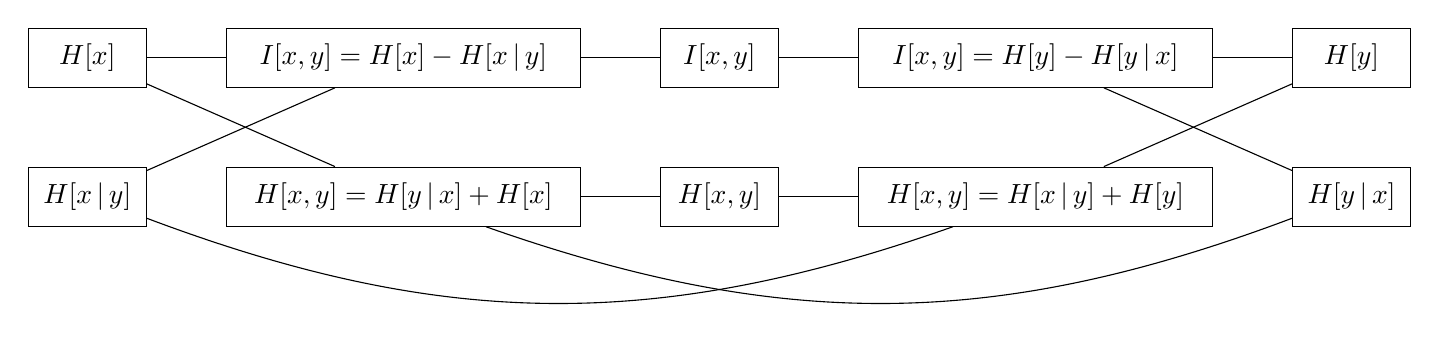
\begin{tikzpicture}[
							quantity/.style = {
								draw,
								rectangle,
								minimum width = 1.5cm,
								minimum height = 0.75cm,
							},
							relation/.style = {
								draw,
								rectangle,
								minimum width = 4.5cm,
								minimum height = 0.75cm,
							}
						]
					\node [quantity] (iXY) {\( I[x, y] \)};
					\node [quantity, below = 1 of iXY] (hXY) {\( H[x, y] \)};

					\node [relation, left = 1 of iXY] (iFromHx) {\( I[x, y] = H[x] - H[x \given y] \)};
					\node [relation, right = 1 of iXY] (iFromHy) {\( I[x, y] = H[y] - H[y \given x] \)};
					\node [relation, left = 1 of hXY] (hXYFromX) {\( H[x, y] = H[y \given x] + H[x] \)};
					\node [relation, right = 1 of hXY] (hXYFromY) {\( H[x, y] = H[x \given y] + H[y] \)};

					\node [quantity, left = 1 of iFromHx] (hX) {\( H[x] \)};
					\node [quantity, right = 1 of iFromHy] (hY) {\( H[y] \)};
					\node [quantity, left = 1 of hXYFromX] (hXgY) {\( H[x \given y] \)};
					\node [quantity, right = 1 of hXYFromY] (hYgX) {\( H[y \given x] \)};

					\draw (iFromHx) to (iXY);
					\draw (iFromHx) to (hX);
					\draw (iFromHx) to (hXgY);

					\draw (iFromHy) to (iXY);
					\draw (iFromHy) to (hY);
					\draw (iFromHy) to (hYgX);

					\draw (hXYFromX) to (hXY);
					\draw (hXYFromX) to (hX);
					\draw (hXYFromX) to[bend right = 20] (hYgX);

					\draw (hXYFromY) to (hXY);
					\draw (hXYFromY) to (hY);
					\draw (hXYFromY) to[bend left = 20] (hXgY);
				\end{tikzpicture}
				\caption{Relations between the entropies and mutual information of two random variables, \(x\) and \(y\).}
				\label{fig:1-39-entropy}
			\end{figure}
		% end

		\subsection{Arithmetic and Geometric Mean  \onestar}
			By applying the logarithm and Jensen's inequality to the geometric mean,
			\begin{equation}
				\log(\, \prod_{i = 1}^{n} x_i \!)^{\!1/n}
					= \frac{1}{n} \log \prod_{i = 1}^{n} x_i
					= \frac{1}{n} \sum_{i = 1}^{n} \log x_i
					\leq \log( \frac{1}{n} \sum_{i = 1}^{n} x_i ),
			\end{equation}
			it can be seen that the logarithm of the arithmetic mean is never less than the logarithm of the geometric mean. By applying the exponential on both sides of the inequality, it follows that also the arithmetic mean itself is never less than the geometric mean.

			\qedeot
		% end

		\subsection{Mutual Information  \onestar}
			The relation \( I[\vec{x}, \vec{y}] = H[\vec{x}] - H[\vec{x} \given \vec{y}] \) can be shown straightforwardly by splitting the integral:
			\begin{align}
				I[\vec{x}, \vec{y}]
					&= -\!\iint\! p(\vec{x}, \vec{y}) \, \log \frac{p(\vec{x}) \, p(\vec{y})}{p(\vec{x}, \vec{y})} \dd{\vec{x}} \dd{\vec{y}} \\
					&= -\!\iint\! p(\vec{x}, \vec{y}) \, \log p(\vec{x}) \dd{\vec{x}} \dd{\vec{y}} + \iint\! p(\vec{x}, \vec{y}) \, \log \frac{p(\vec{x}, \vec{y})}{p(\vec{y})} \dd{\vec{x}} \dd{\vec{y}} \\
					&= -\!\iint\! p(\vec{x}, \vec{y}) \, \log p(\vec{x}) \dd{\vec{x}} \dd{\vec{y}} + \iint\! p(\vec{x}, \vec{y}) \, \log p(\vec{x} \given \vec{y}) \dd{\vec{x}} \dd{\vec{y}} \\
					&= H[\vec{x}] - H[\vec{x} \given \vec{y}]
			\end{align}
			This concludes the proof. Showing \( I[\vec{x}, \vec{y}] = H[\vec{y}] - H[\vec{y} \given \vec{x}] \) is analogous.

			\qedeot
		% end
	% end

	\section{Probability Distributions}
		\subsection{Mean, Variance, and Entropy of Bernoulli Distribution  \onestar}
			As the Bernoulli distribution is over a finite set of discrete values for \(x\), it is easy to show that it is normalized and to evaluate the mean and variance:
			\begin{equation}
				\sum_{x = 0}^{1} \mathrm{Bern}(x \given \mu)
					= \mathrm{Bern}(0 \given \mu) + \mathrm{Bern}(1 \given \mu)
					= \mu^0 (1 - \mu)^{1 - 0} + \mu^1 (1 - \mu)^{1 - 1}
					= (1 - \mu) + \mu
					= 1
			\end{equation}
			\begin{equation}
				\E[x]
					= \sum_{x = 0}^{1} x \,\mathrm{Bern}(x \given \mu)
					= 0 \cdot \mu^0 (1 - \mu)^{1 - 0} + 1 \cdot \mu^1 (1 - \mu)^{1 - 1}
					= \mu
			\end{equation}
			\begin{equation}
				\Var[x]
					= \E\big[x^2\big] - \E^2[x]
					= \sum_{x = 0}^{1} x^2 \,\mathrm{Bern}(x \given \mu) - \mu^2
					= \mu - \mu^2
					= \mu (1 - \mu)
			\end{equation}
			Additionally, the entropy is given by
			\begin{align}
				H[x]
					&= -\sum_{x = 0}^{1} \mathrm{Bern}(x \given \mu) \, \log \mathrm{Bern}(x \given \mu) \\
					&= -\sum_{x = 0}^{1} \mu^x (1 - \mu)^{1 - x} \big( x \log \mu + (1 - x) \log (1 - \mu) \big) \\
					&= -(1 - \mu) \log (1 - \mu) - \mu \log \mu.
			\end{align}
			This concludes the task.

			\eot
		% end

		\subsection{Symmetric Bernoulli Distribution  \twostar}
			It is easy to see by summation that the symmetric Bernoulli distribution
			\begin{equation}
				p(x \given \mu) = \bigg( \frac{1 - \mu}{2} \bigg)^{(1 - x) / 2} \bigg( \frac{1 + \mu}{2} \bigg)^{(1 + x) / 2}
			\end{equation}
			is indeed normalized:
			\begin{equation}
				\sum_{x \,=\, \pm 1} p(x \given \mu)
					= \sum_{x \,=\, \pm 1} \bigg( \frac{1 - \mu}{2} \bigg)^{(1 - x) / 2} \bigg( \frac{1 + \mu}{2} \bigg)^{(1 + x) / 2}
					= \frac{1 - \mu}{2} + \frac{1 + \mu}{2}
					= \frac{1}{2} (1 - \mu + 1 + \mu)
					= 1
			\end{equation}
			Similarly, its mean is given by
			\begin{equation}
				\E[x]
					= \sum_{x \,=\, \pm 1} x \, p(x \given \mu)
					= -1 \cdot \frac{1 - \mu}{2} + 1 \cdot \frac{1 + \mu}{2}
					= \frac{1}{2} (-1 + \mu + 1 + \mu)
					= \mu.
			\end{equation}
			which is equivalent to the mean of the Bernoulli distribution. But, as \( (-1)^2 = 1 \), the variance vanishes:
			\begin{equation}
				\Var[x]
					= \E\big[x^2\big] - \E^2[x]
					= \mu^2 - \mu^2
					= 0
			\end{equation}
			Evaluating the entropy is also straightforward:
			\begin{align}
				H[x]
					&= -\!\!\sum_{x \,=\, \pm 1} p(x \given \mu) \, \log p(x \given \mu) \\
					&= -\!\!\sum_{x \,=\, \pm 1} \bigg( \frac{1 - \mu}{2} \bigg)^{(1 - x) / 2} \bigg( \frac{1 + \mu}{2} \bigg)^{(1 + x) / 2} \bigg( \frac{1 - x}{2} \big(\! \log(1 - \mu) - \log 2 \big) + \frac{1 + x}{2} \big(\! \log(1 + \mu) - \log 2 \big) \!\bigg) \\
					&= -\frac{1 - \mu}{2} \big(\! \log(1 - \mu) - \log 2 \big) - \frac{1 + \mu}{2} \big(\! \log(1 + \mu) - \log 2 \big) \\
					&= -\frac{1 - \mu}{2} \log(1 - \mu) - \frac{1 + \mu}{2} \log(1 + \mu) + \frac{1}{2} \log 2 - \frac{\mu}{2} \log 2 + \frac{1}{2} \log 2 + \frac{\mu}{2} \log 2 \\
					&= -\frac{1 - \mu}{2} \log(1 - \mu) - \frac{1 + \mu}{2} \log(1 + \mu) + \log 2
			\end{align}
			This concludes the task.

			\eot
		% end

		\subsection{Normalization of Binomial Distribution  \twostar}
			by using the property \( (k + 1)! = (k + 1) \cdot k! \) of the factorial, the first relation is easy to show:
			\begin{equation}
				\begin{aligned}
					{ N \choose m } + { N \choose m - 1 }
						&= \frac{N!}{(N - m)! \, m!} + \frac{N!}{(N - m + 1)! \, (m - 1)!}
						 = \frac{N!}{(N - m)! \, m!} + \frac{m \, N!}{(N - m + 1) \, (N - m)! \, m!} \\
						&= \frac{(N - m + 1) \, N!}{(N - m + 1) \, (N - m)! \, m!} + \frac{m \, N!}{(N - m + 1) \, (N - m)! \, m!}
						 = \frac{(N - m + 1) \, N! + m \, N!}{(N - m + 1) \, (N - m)! \, m!} \\
						&= \frac{N \, N! - m \, N! + N! + m \, N!}{(N - m + 1) \, (N - m)! \, m!}
						 = \frac{N \, N! + N!}{(N - m + 1) \, (N - m)! \, m!}
						 = \frac{(N + 1) \, N!}{(N - m + 1) \, (N - m)! \, m!} \\
						&= \frac{(N + 1)!}{(N - m + 1) \, (N - m)! \, m!}
						 = \frac{(N + 1)!}{(N + 1 - m)! \, m!}
						 = { N + 1 \choose m }
				\end{aligned}
			\end{equation}
			\qed

			To now show \( (1 + x)^N = \sum_{m = 0}^{N} { N \choose m } x^m \), first consider \( N = 1 \). Then
			\begin{equation}
				\sum_{m = 0}^{N} { N \choose m } x^m
					= \sum_{m = 0}^{1} { 1 \choose m } x^m
					= { 1 \choose 0 } + { 1 \choose 1 } x
					= 1 + x
					= (1 + x)^1
					= (1 + x)^N.
			\end{equation}
			Let now \(N\) be any arbitrary natural number such that the above relation holds. Then for \(N + 1\), the following holds
			\begin{align}
				(1 + x)^{N + 1}
					&= (1 + x) \, (1 + x)^N
					 = (1 + x) \sum_{m = 0}^{N} { N \choose m } x^m
					 = \sum_{m = 0}^{N} { N \choose m } x^m + x \sum_{m = 0}^{N} { N \choose m } x^m \\
					&= \sum_{m = 0}^{N} { N \choose m } x^m + \sum_{m = 0}^{N} { N \choose m } x^{m + 1}
					 = \sum_{m = 0}^{N} { N \choose m } x^m + \sum_{m = 1}^{N + 1} { N \choose m - 1 } x^m \\
					&= \sum_{m = 0}^{N} { N \choose m } x^m + \sum_{m = 1}^{N + 1} { N \choose m - 1 } x^m + { N \choose N + 1 } x^{N + 1} - { N \choose N + 1 } x^{N + 1} \\
					&= \sum_{m = 0}^{N + 1} { N \choose m } x^m + \sum_{m = 1}^{N + 1} { N \choose m - 1 } x^m - { N \choose N + 1 } x^{N + 1} - { N \choose 0 } x^0 + { N \choose 0 } x^0 \\
					&= \sum_{m = 0}^{N + 1} { N \choose m } x^m + \sum_{m = 1}^{N + 1} { N \choose m - 1 } x^m - { N \choose N + 1 } x^{N + 1} + { N \choose -1 } x^0 - { N \choose -1 } x^0 \\
					&= \sum_{m = 0}^{N + 1} { N \choose m } x^m + \sum_{m = 0}^{N + 1} { N \choose m - 1 } x^m - { N \choose N + 1 } x^{N + 1} - { N \choose -1 } x^0 \\
					&= \sum_{m = 0}^{N + 1} \Bigg(\! { N \choose m } + { N \choose m - 1 } \!\Bigg) x^m - { N \choose N + 1 } x^{N + 1} - { N \choose -1 } x^0 \\
					&= \sum_{m = 0}^{N + 1} { N + 1 \choose m } x^m - \underbrace{{ N \choose N + 1 }}_{=\, 0} x^{N + 1} - \underbrace{{ N \choose -1 }}_{=\, 0} x^0
					 = \sum_{m = 0}^{N + 1} { N + 1 \choose m } x^m,
			\end{align}
			where in the second step the assumption was used that the relation holds for any \(N\). This it follows that the relation holds for all natural \(N\).
			\qed

			It is now straightforward to show that the Binomial distribution is normalized
			\begin{align}
				\sum_{m = 0}^{N} { N \choose m } \mu^m (1 - \mu)^{N - m}
					&= \sum_{m = 0}^{N} { N \choose m } \mu^m (1 - \mu)^N (1 - \mu)^{-m}
					 = (1 - \mu)^N \sum_{m = 0}^{N} { N \choose m } \bigg( \frac{\mu}{1 - \mu} \bigg)^m \\
					&= (1 - \mu)^N \,\bigg(\! 1 + \frac{\mu}{1 - \mu} \bigg)^N
					 = \big( 1 - \mu + \mu \big)^N
					 = 1^N
					 = 1,
			\end{align}
			where in the third step the binomial theorem was invoked.

			\eot
		% end

		\subsection{Mean and Variance of Binomial Distribution  \twostar}
			The derivative of the left hand side of the normalization condition w.r.t. \(\mu\) is given as
			\begin{align}
				 &\, \pdv{\mu} \sum_{m = 0}^{N} { N \choose m } \mu^m (1 - \mu)^{N - m} \\
				=&\, \sum_{m = 0}^{N} { N \choose m } \Big( m \mu^{m - 1} (1 - \mu)^{N - m} - (N - m) \mu^m (1 - \mu)^{N - m - 1} \Big) \\
				=&\, \frac{1}{\mu} \sum_{m = 0}^{N} { N \choose m } m \mu^m (1 - \mu)^{N - m} - \frac{N}{1 - \mu} \sum_{m = 0}^{N} { N \choose m } \mu^m (1 - \mu)^{N - m} + \frac{1}{1 - \mu} \sum_{m = 0}^{N} { N \choose m } m \mu^m (1 - \mu)^{N - m} \\
				=&\, \frac{1}{\mu} \E[m] - \frac{N}{1 - \mu} + \frac{1}{1 - \mu} \E[m]
					\propto (1 - \mu) \, \E[m] - N \mu + \mu \, \E[m]
					= \E[m] - N \mu
			\end{align}
			By equating this result with zero (the derivative of the right hand side), an expression for the expectation can be obtained as \( \E[m] = N \mu \). To find an expression for the variance, the second derivative of the normalization condition is used analogously. However, the derivation is rather lengthy:
			\begin{align}
				 &\, \pdv[2]{\mu} \sum_{m = 0}^{N} { N \choose m } \mu^m (1 - \mu)^{N - m} \\
				=&\, \pdv{\mu} \sum_{m = 0}^{N} { N \choose m } \Big(
						  m \mu^{m - 1} (1 - \mu)^{N - m}
						- (N - m) \mu^m (1 - \mu)^{N - m - 1}
					\Big) \\
				=&\, \sum_{m = 0}^{N} { N \choose m } \Big(
						  (m - 1) m \mu^{m - 2} (1 - \mu)^{N - m}
						- 2 (N - m) m \mu^{m - 1} (1 - \mu)^{N - m - 1} \\&\qquad\qquad\qquad
						+ (N - m) (N - m - 1) \mu^m (1 - \mu)^{N - m - 2} \\
				=&\, \sum_{m = 0}^{N} { N \choose m } \Big(
						  (m^2 - m) \mu^{m - 2} (1 - \mu)^{N - m}
						- 2 (Nm - m^2) \mu^{m - 1} (1 - \mu)^{N - m - 1} \\&\qquad\qquad\qquad
						+ (N^2 + m^2 - 2Nm - N + m) \mu^m (1 - \mu)^{N - m - 2} \\
				=&\, \sum_{m = 0}^{N} { N \choose m } \Big(
						  \frac{1}{\mu^2} (m^2 - m) \mu^m (1 - \mu)^{N - m}
						- \frac{2}{\mu (1 - \mu)} (Nm - m^2) \mu^m (1 - \mu)^{N - m} \\&\qquad\qquad\qquad
						+ \frac{1}{(1 - \mu)^2} (N^2 + m^2 - 2Nm - N + m) \mu^m (1 - \mu)^{N - m}
					\Big) \\
				\propto&\, \sum_{m = 0}^{N} { N \choose m } \Big(
						  (1 - \mu)^2 (m^2 - m) \mu^m (1 - \mu)^{N - m}
						- 2 (1 - \mu) \mu (Nm - m^2) \mu^m (1 - \mu)^{N - m} \\&\qquad\qquad\qquad
						+ \mu^2 (N^2 + m^2 - 2Nm - N + m) \mu^m (1 - \mu)^{N - m}
					\Big) \\
				=&\,  (1 - \mu)^2 \, \E\big[ m^2 - m \big]
					- 2 (1 - \mu) \mu \, \E\big[ Nm - m^2 \big]
					+ \mu^2 \, \E\big[ N^2 + m^2 - 2Nm - N + m \big] \\
				=&\,  (1 - \mu)^2 \Big( \E\big[m^2\big] - N\mu \Big)
					- 2 (1 - \mu) \mu \Big( N^2 \mu - \E\big[m^2\big] \Big)
					+ \mu^2 \Big( N^2 + \E\big[m^2\big] - 2 N^2 \mu - N + N \mu \Big) \\
				=&\,  (1 + \mu^2 - 2 \mu) \Big( \E\big[m^2\big] - N\mu \Big)
					- 2 (\mu - \mu^2) \Big( N^2 \mu - \E\big[m^2\big] \Big)
					+ \mu^2 \Big( N^2 + \E\big[m^2\big] - 2 N^2 \mu - N + N \mu \Big) \\
				=&\,  \Big( \E\big[m^2\big] - N\mu \Big)
					+ \mu^2 \Big( \E\big[m^2\big] - N\mu \Big)
					- 2 \mu \Big( \E\big[m^2\big] - N\mu \Big) \\&\qquad\qquad\qquad
					- 2 \mu \Big( N^2 \mu - \E\big[m^2\big] \Big)
					+ 2 \mu^2 \Big( N^2 \mu - \E\big[m^2\big] \Big)
					+ \mu^2 \Big( N^2 + \E\big[m^2\big] - 2 N^2 \mu - N + N \mu \Big) \\
				=&\,  \E\big[m^2\big] - N\mu
					+ \mu^2 \E\big[m^2\big] - N \mu^3
					- 2 \mu \E\big[m^2\big] + 2 N \mu^2 \\&\qquad\qquad\qquad
					- 2 N^2 \mu^2 + 2 \mu \E\big[m^2\big]
					+ 2 N^2 \mu^3 - 2 \mu^2 \E\big[m^2\big]
					+ N^2 \mu^2 + \mu^2 \E\big[m^2\big] - 2 N^2 \mu^3 - N \mu^2 + N \mu^3 \\
				=&\,  \E\big[m^2\big] - N\mu
					- N \mu^3
					+ 2 N \mu^2
					- 2 N^2 \mu^2
					+ 2 N^2 \mu^3
					+ N^2 \mu^2 - 2 N^2 \mu^3 - N \mu^2 + N \mu^3 \\
				=&\,  \E\big[m^2\big]
					- N \mu
					+ (2 N - 2 N^2 + N^2 - N) \mu^2
					+ (-N + 2 N^2 - 2 N^2 + N) \mu^3 \\
				=&\,  \E\big[m^2\big] - N \mu + (N - N^2) \mu^2 \\
				=&\,  \E\big[m^2\big] - N \mu + N \mu^2 - N^2 \mu^2 \\
				=&\,  \E\big[m^2\big] - \E^2[m] - N \mu + N \mu^2 \\
				=&\,  \Var[m] - N \mu + N \mu^2 \\
				=&\,  \Var[m] - N \mu (1 - \mu)
			\end{align}
			By equating this result with zero (the left hand side), the expression \( \Var[m] = N \mu (1 - \mu) \) is obtained.

			\eot
		% end

		\subsection{Normalization of Beta Distribution  \twostar}
			To show that the Beta distribution is normalized, i.e., that
			\begin{equation}
				\int_{0}^{1}\! \mu^{a - 1} (1 - \mu)^{b - 1} \dd{\mu} = \frac{\Gamma(a + b)}{\Gamma(a) \Gamma(b)}
			\end{equation}
			holds, the quantity \( \Gamma(a) \Gamma(b) \) has to be computed. By plugging the solution
			\begin{align}
				\Gamma(a) \Gamma(b)
					&= \int_{x \,=\, 0}^{\infty}\! e^{-x} x^{a - 1} \dd{x} \int_{y \,=\, 0}^{\infty}\! e^{-y} y^{b - 1} \dd{y}
					 = \int_{x \,=\, 0}^{\infty} \int_{y \,=\, 0}^{\infty}\! e^{-(x + y)} x^{a - 1} y^{b - 1} \dd{y} \dd{x} \\
					&= \int_{x \,=\, 0}^{\infty} \int_{t \,=\, 0}^{\infty}\! e^{-t} x^{a - 1} (t - x)^{b - 1} \dd{t} \dd{x}
					 = \int_{t \,=\, 0}^{\infty} \int_{x \,=\, 0}^{1}\! e^{-t} x^{a - 1} (t - x)^{b - 1} \dd{x} \dd{t} \\
					&= \int_{t \,=\, 0}^{\infty} \int_{\mu \,=\, 0}^{1}\! e^{-t} (t\mu)^{a - 1} (t - t\mu)^{b - 1} t \dd{\mu} \dd{t}
					 = \int_{t \,=\, 0}^{\infty} \int_{\mu \,=\, 0}^{1}\! e^{-t} t t^{a - 1} t^{b - 1} \mu^{a - 1} (1 - \mu)^{b - 1} \dd{\mu} \dd{t} \\
					&= \int_{t \,=\, 0}^{\infty} \int_{\mu \,=\, 0}^{1}\! e^{-t} t^{a + b - 1} \mu^{a - 1} (1 - \mu)^{b - 1} \dd{\mu} \dd{t}
					 = \Gamma(a + b) \int_{\mu \,=\, 0}^{1}\! \mu^{a - 1} (1 - \mu)^{b - 1} \dd{\mu}
			\end{align}
			into the normalization condition, it can be seen that the left and right hand side are indeed equal. Hence, the Beta distribution is normalized.

			\qedeot
		% end

		\subsection{Mean, Variance, and Mode of Beta Distribution  \onestar}
			To evaluate the mean, the result of the previous task can be leveraged:
			\begin{align}
				\E[\mu]
					&= \frac{\Gamma(a) \Gamma(b)}{\Gamma(a + b)} \int_{0}^{1}\! \mu \mu^{a - 1} (1 - \mu)^{b - 1} \dd{\mu}
					 = \frac{\Gamma(a) \Gamma(b)}{\Gamma(a + b)} \int_{0}^{1}\! \mu^{a + 1 - 1} (1 - \mu)^{b - 1} \dd{\mu} \\
					&= \frac{\Gamma(a) \Gamma(b)}{\Gamma(a + b)} \frac{\Gamma(a + 1) \Gamma(b)}{\Gamma(a + 1 + b)}
					 = \frac{\Gamma(a) \Gamma(b)}{\Gamma(a + b)} \frac{a \Gamma(a) \Gamma(b)}{(a + b) \Gamma(a + b)}
					 = \frac{a}{a + b}
			\end{align}
			To evaluate the variance, it is at first helpful to evaluate the second moment:
			\begin{align}
				\E\big[\mu^2\big]
					&= \frac{\Gamma(a) \Gamma(b)}{\Gamma(a + b)} \int_{0}^{1}\! \mu^2 \mu^{a - 1} (1 - \mu)^{b - 1} \dd{\mu}
					 = \frac{\Gamma(a) \Gamma(b)}{\Gamma(a + b)} \int_{0}^{1}\! \mu^{a + 2 - 1} (1 - \mu)^{b - 1} \dd{\mu} \\
					&= \frac{\Gamma(a) \Gamma(b)}{\Gamma(a + b)} \frac{\Gamma(a + 2) \Gamma(b)}{\Gamma(a + 2 + b)}
					 = \frac{\Gamma(a) \Gamma(b)}{\Gamma(a + b)} \frac{a (a + 1) \Gamma(a) \Gamma(b)}{(a + b) (a + b + 1) \Gamma(a + b)}
					 = \frac{a (a + 1)}{(a + b) (a + b + 1)}
			\end{align}
			This can then be plugged into the variance, combined with the squared mean:
			\begin{align}
				\Var[\mu]
					&= \E\big[\mu^2\big] - \E^2[\mu]
					 = \frac{a (a + 1)}{(a + b) (a + b + 1)} - \frac{a^2}{(a + b)^2}
					 = \frac{a (a + 1) (a + b)}{(a + b)^2 (a + b + 1)} - \frac{a^2 (a + b + 1)}{(a + b)^2 (a + b + 1)} \\
					&= \frac{a (a + 1) (a + b) - a^2 (a + b + 1)}{(a + b)^2 (a + b + 1)}
					 = \frac{a^3 - a^3 + a^2 b - a^2 b + a^2 - a^2 + ab}{(a + b)^2 (a + b + 1)}
					 = \frac{ab}{(a + b)^2 (a + b + 1)}
			\end{align}
			To proof that \( \mode[\mu] = (a - 1)/(a + b - 2) \), this value has to be plugged into the derivative of the density function w.r.t. \(\mu\):
			\begin{align}
				\pdv{\mu} \mu^{a - 1} (1 - \mu)^{b - 1}
					=&\, (a - 1) \mu^{a - 2} (1 - \mu)^{b - 1} - (b - 1) \mu^{a - 1} (1 - \mu)^{b - 2} \\
					\to&\, (a - 1) \bigg( \frac{a - 1}{a + b - 2} \bigg)^{a - 2} \bigg( \frac{b - 1}{a + b - 2} \bigg)^{b - 1} - (b - 1) \bigg( \frac{a - 1}{a + b - 2} \bigg)^{a - 1} \bigg( \frac{b - 1}{a + b - 2} \bigg)^{b - 2} \\
					=&\, (a - 1) \frac{(a - 1)^{a - 2}}{(a + b - 2)^{a - 2}} \frac{(b - 1)^{b - 1}}{(a + b - 2)^{b - 1}} - (b - 1) \frac{(a - 1)^{a - 1}}{(a + b - 2)^{a - 1}} \frac{(b - 1)^{b - 2}}{(a + b - 2)^{b - 2}} \\
					=&\, (a - 1) \frac{(a - 1)^{a - 2} (b - 1)^{b - 1}}{(a + b - 2)^{a + b - 3}} - (b - 1) \frac{(a - 1)^{a - 1} (b - 1)^{b - 2}}{(a + b - 2)^{a + b - 3}} \\
					=&\, \frac{(a - 1)^{a - 1} (b - 1)^{b - 1}}{(a + b - 2)^{a + b - 3}} - \frac{(a - 1)^{a - 1} (b - 1)^{b - 1}}{(a + b - 2)^{a + b - 3}}
					 = 0
			\end{align}
			Hence, \( \mode[\mu] = (a - 1)/(a + b - 2) \). While plugging this result in, the relation \( 1 - (a - 1)/(a + b - 2) = (b - 1)/(a + b - 2) \) was used.

			\eot
		% end

		\subsection{Posterior of Binomial Random Variable  \twostar}
			The posterior distribution
			\begin{equation}
				p(\mu \given m, \ell, a, b) \propto \mu^{a + m - 1} (1 - \mu)^{b + \ell - 1}
			\end{equation}
			over the parameter \(\mu\) of a Binomial distribution given the conjugate Beta prior is also a Beta distribution \( p(\mu \given m, \ell, a, b) = \mathrm{Beta}(\mu \given \hat{a}, \hat{b}) \) with \( \hat{a} = a + m \) and \( \hat{b} = b + \ell \) where \(a\), \(b\) are the parameters of the prior. The mean of the posterior is therefore given by
			\begin{align}
				\E_{\mu \sim p(\cdot \given m, \ell, a, b)}[\mu]
					&= \frac{\hat{a}}{\hat{a} + \hat{b}}
					 = \frac{a + m}{a + b + m + \ell}
					 = \frac{a}{a + b + m + \ell} + \frac{m}{a + b + m + \ell} \\
					&= \frac{(a + b) (m + \ell)}{(a + b) (m + \ell)} \frac{a}{a + b + m + \ell} + \frac{(a + b) (m + \ell)}{(a + b) (m + \ell)} \frac{m}{a + b + m + \ell} \\
					&= \frac{(a + b) (m + \ell)}{(a + b + m + \ell) (m + \ell)} \frac{a}{a + b} + \frac{(a + b) (m + \ell)}{(a + b) (a + b + m + \ell)} \frac{m}{m + \ell} \\
					&= \frac{a + b}{a + b + m + \ell} \frac{a}{a + b} + \frac{m + \ell}{a + b + m + \ell} \frac{m}{m + \ell}.
			\end{align}
			It remains to be shown that the coefficient of the maximum likelihood estimate equals one minus the factor of the prior:
			\begin{equation}
				1 - \frac{m + \ell}{a + b + m + \ell}
					= \frac{a + b + m + \ell}{a + b + m + \ell} - \frac{m + \ell}{a + b + m + \ell}
					= \frac{a + b + m + \ell - m - \ell}{a + b + m + \ell}
					= \frac{a + b}{a + b + m + \ell}
			\end{equation}
			Thus, the posterior comprises between the prior and the maximum likelihood solution.

			\qedeot
		% end

		\subsection{Conditional Expectation and Variance  \onestar}
			By using \( p(x, y) = p(x \given y) \, p(y) \), the first statement can be shown:
			\begin{equation}
				\E_y\big[ \E_x[x \given y] \big]
					= \int\! \E_x[x \given y] \, p(y) \dd{y}
					= \iint\! x \, p(x \given y) \, p(y) \dd{x} \dd{y}
					= \iint\! x \, p(x, y) \dd{x} \dd{y}
					= \E[x]
			\end{equation}
			Using this result, the second statement is also straightforward:
			\begin{align}
				\E_y\big[ \Var_x[x \given y] \big] + \Var_y\big[ \E_x[x \given y] \big]
					&= \Big( \E_y\big[ \E_x\big[x^2 \biggiven y\big] - \E_x^2[x \given y] \big] \Big) + \Big( \E_y\big[ \E_x^2[x \given y] \big] - \E_y^2\big[ \E_x[x \given y] \big] \Big) \\
					&= \Big( \E\big[x^2\big] - \E_y\big[ \E_x^2[x \given y] \big] \Big) + \Big( \E_y\big[ \E_x^2[x \given y] \big] - \E^2[x] \Big)
					 = \E\big[x^2\big] - \E^2[x]
					 = \Var[x]
			\end{align}
			Here, \( \E_y\big[ \E_x\big[x^2 \biggiven y\big] \big] = \E\big[x^2\big] \) was used which can be shown analogous to the mean.

			\eot
		% end

		\subsection{Normalization of Dirichlet Distribution  \threestar}
			% TODO: 2.9 (***): Task: Norm. of Dirichlet
		% end

		\subsection{Mean, Variance, and Covariance of Dirichlet Distribution  \twostar}
			Evaluating the expression for the mean is analogous to the mean of the Beta distribution:
			\begin{align}
				\E[\mu_j]
					&= \frac{\Gamma(\alpha_0)}{\prod_{k = 1}^{K} \Gamma(\alpha_k)} \int_{0}^{1}\! \mu_j \prod_{k = 1}^{K} \mu_k^{\alpha_k - 1} \dd{\vec{\mu}}
					 = \frac{\Gamma(\alpha_0)}{\prod_{k = 1}^{K} \Gamma(\alpha_k)} \int_{0}^{1}\! \prod_{k = 1}^{K} \mu_k^{\alpha_k + \delta_{kj} - 1} \dd{\vec{\mu}} \\
					&= \frac{\Gamma(\alpha_0)}{\prod_{k = 1}^{K} \Gamma(\alpha_k)} \frac{\prod_{k = 1}^{K} \Gamma(\alpha_k + \delta_{kj})}{\Gamma(\alpha_0 + 1)}
					 = \frac{\Gamma(\alpha_0)}{\prod_{k = 1}^{K} \Gamma(\alpha_k)} \frac{\alpha_j \prod_{k = 1}^{K} \Gamma(\alpha_k)}{\alpha_0 \Gamma(\alpha_0)}
					 = \frac{\alpha_j}{\alpha_0}
			\end{align}
			Analogously to the Beta distribution, for evaluating the variance firstly the second moment has to be evaluated,
			\begin{align}
				\E\big[\mu_j^2\big]
					&= \frac{\Gamma(\alpha_0)}{\prod_{k = 1}^{K} \Gamma(\alpha_k)} \int_{0}^{1}\! \mu_j^2 \prod_{k = 1}^{K} \mu_k^{\alpha_k - 1} \dd{\vec{\mu}}
					 = \frac{\Gamma(\alpha_0)}{\prod_{k = 1}^{K} \Gamma(\alpha_k)} \int_{0}^{1}\! \prod_{k = 1}^{K} \mu_k^{\alpha_k + 2\delta_{kj} - 1} \dd{\vec{\mu}} \\
					&= \frac{\Gamma(\alpha_0)}{\prod_{k = 1}^{K} \Gamma(\alpha_k)} \frac{\prod_{k = 1}^{K} \Gamma(\alpha_k + 2\delta_{kj})}{\Gamma(\alpha_0 + 2)}
					 = \frac{\Gamma(\alpha_0)}{\prod_{k = 1}^{K} \Gamma(\alpha_k)} \frac{\alpha_j (\alpha_j + 1) \prod_{k = 1}^{K} \Gamma(\alpha_k)}{\alpha_0 (\alpha_0 + 1) \Gamma(\alpha_0)}
					 = \frac{\alpha_j (\alpha_j + 1)}{\alpha_0 (\alpha_0 + 1)},
			\end{align}
			and afterwards the variance:
			\begin{equation}
				\Var[\mu_j]
					= \E\big[\mu_j^2\big] - \E^2[\mu_j]
					= \frac{\alpha_j (\alpha_j + 1)}{\alpha_0 (\alpha_0 + 1)} - \frac{\alpha_j^2}{\alpha_0^2}
					= \frac{\alpha_0 \alpha_j (\alpha_j + 1)}{\alpha_0^2 (\alpha_0 + 1)} - \frac{\alpha_j^2 (\alpha_0 + 1)}{\alpha_0^2 (\alpha_0 + 1)}
%					= \frac{\alpha_0 \alpha_j^2 + \alpha_0 \alpha_j - \alpha_0 \alpha_j^2 - \alpha_j^2}{\alpha_0^2 (\alpha_0 + 1)}
					= \frac{\alpha_j (\alpha_0- \alpha_j)}{\alpha_0^2 (\alpha_0 + 1)}
			\end{equation}
			For evaluating the covariance, first the second moment \( \E[\mu_j \mu_\ell] \) with \( j \neq \ell \) has to be evaluated:
			\begin{align}
				\E[\mu_j]
					&= \frac{\Gamma(\alpha_0)}{\prod_{k = 1}^{K} \Gamma(\alpha_k)} \int_{0}^{1}\! \mu_j \mu_\ell \prod_{k = 1}^{K} \mu_k^{\alpha_k - 1} \dd{\vec{\mu}}
					 = \frac{\Gamma(\alpha_0)}{\prod_{k = 1}^{K} \Gamma(\alpha_k)} \int_{0}^{1}\! \prod_{k = 1}^{K} \mu_k^{\alpha_k + \delta_{kj} + \delta_{k\ell} - 1} \dd{\vec{\mu}} \\
					&= \frac{\Gamma(\alpha_0)}{\prod_{k = 1}^{K} \Gamma(\alpha_k)} \frac{\prod_{k = 1}^{K} \Gamma(\alpha_k + \delta_{kj} + \delta_{k\ell})}{\Gamma(\alpha_0 + 2)}
					 = \frac{\Gamma(\alpha_0)}{\prod_{k = 1}^{K} \Gamma(\alpha_k)} \frac{\alpha_j \alpha_\ell \prod_{k = 1}^{K} \Gamma(\alpha_k)}{\alpha_0 (\alpha_0 + 1) \Gamma(\alpha_0)}
					 = \frac{\alpha_j \alpha_\ell}{\alpha_0 (\alpha_0 + 1)}
			\end{align}
			Plugging this into the covariance yields
			\begin{equation}
				\cov[\mu_j, \mu_\ell]
					= \E[\mu_j \mu_\ell] - \E[\mu_j] \, \E[\mu_\ell]
					= \frac{\alpha_j \alpha_\ell}{\alpha_0 (\alpha_0 + 1)} - \frac{\alpha_j}{\alpha_0} \frac{\alpha_\ell}{\alpha_0}
%					= \frac{\alpha_j \alpha_\ell}{\alpha_0 (\alpha_0 + 1)} - \frac{\alpha_j \alpha_\ell}{\alpha_0^2}
					= \frac{\alpha_0 \alpha_j \alpha_\ell}{\alpha_0^2 (\alpha_0 + 1)} - \frac{\alpha_j \alpha_\ell (\alpha_0 + 1)}{\alpha_0^2 (\alpha_0 + 1)}
%					= \frac{\alpha_0 \alpha_j \alpha_\ell - \alpha_0 \alpha_j \alpha_\ell - \alpha_j \alpha_\ell}{\alpha_0^2 (\alpha_0 + 1)}
					= \frac{-\alpha_j \alpha_\ell}{\alpha_0^2 (\alpha_0 + 1)}.
			\end{equation}
			This is the expression for the covariance given in the task.

			\eot
		% end

		\subsection{Expectation of Logarithm under Dirichlet Distribution  \onestar}
			By taking the derivative of the \(\mu\)-dependent term of the Dirichlet distribution, it can be seen that
			\begin{equation}
				\pdv{\alpha_j} \prod_{k = 1}^{K} \mu_k^{\alpha_k - 1}
					= \bigg( \pdv{\alpha_j} \mu_j^{\alpha_j - 1} \bigg) \prod_{\substack{k = 1 \\ k \neq j}}^{K} \mu_k^{\alpha_k - 1}
					= \log(\mu_j) \mu_j^{\alpha_j - 1} \prod_{\substack{k = 1 \\ k \neq j}}^{K} \mu_k^{\alpha_k - 1}
					= \log(\mu_j) \prod_{k = 1}^{K} \mu_k^{\alpha_k - 1}.
			\end{equation}
			But this quantity also appears in the expectation \( \E[\log \mu_j] \). Hence, by plugging it in
			\begin{align}
				\E[\log \mu_j]
					&= \frac{\Gamma(\alpha_0)}{\prod_{k = 1}^{K} \Gamma(\alpha_k)} \int_{0}^{1}\! \log(\mu_j) \prod_{k = 1}^{K} \mu_k^{\alpha_k - 1} \dd{\vec{\mu}}
					 = \frac{\Gamma(\alpha_0)}{\prod_{k = 1}^{K} \Gamma(\alpha_k)} \pdv{\alpha_j} \int_{0}^{1}\! \prod_{k = 1}^{K} \mu_k^{\alpha_k - 1} \dd{\vec{\mu}} \\
					&= \frac{\Gamma(\alpha_0)}{\prod_{k = 1}^{K} \Gamma(\alpha_k)} \pdv{\alpha_j} \frac{\prod_{k = 1}^{K} \Gamma(\alpha_k)}{\Gamma(\alpha_0)}
					 = \pdv{\alpha_j} \log \frac{\prod_{k = 1}^{K} \Gamma(\alpha_k)}{\Gamma(\alpha_0)}
					 = \pdv{\alpha_j} \Bigg( \sum_{k = 1}^{K} \log \Gamma(\alpha_k) - \log \Gamma(\alpha_0) \!\Bigg) \\
					&= \dv{\alpha_j} \log \Gamma(\alpha_j) - \dv{\alpha_j} \log \Gamma(\alpha_0)
					 = \psi(\alpha_j) - \psi(\alpha_0),
			\end{align}
			the result from the task is obtained with \(\psi(a) \coloneqq \dv*{a} \log \Gamma(a) \).

			\eot
		% end

		\subsection{Normalization of Uniform Distribution  \onestar}
			It is easy to see that the uniform distribution is normalized:
			\begin{equation}
				\int_{a}^{b}\! U(x \given a, b) \dd{x}
					= \int_{a}^{b}\! \frac{1}{b - a} \dd{x}
					= \bigg[ \frac{x}{b - a} \bigg]_{x \,=\, a}^{x \,=\, b}
					= \frac{b}{b - a} - \frac{a}{b - a}
					= \frac{b - a}{b - a}
					= 1
			\end{equation}
			Also the first and second moment can be evaluates easily:
			\begin{equation}
				\E[x]
					= \int_{a}^{b}\! \frac{x}{b - a} \dd{x}
					= \frac{1}{2} \bigg[ \frac{x^2}{b - a} \bigg]_{x \,=\, a}^{x \,=\, b}
					= \frac{1}{2} \bigg[ \frac{b^2}{b - a} - \frac{a^2}{b - a} \bigg]
					= \frac{1}{2} \frac{b^2 - a^2}{b - a}
					= \frac{1}{2} \frac{(b + a) (b - a)}{b - a}
					= \frac{a + b}{2}
			\end{equation}
			\begin{equation}
				\E\big[x^2\big]
					= \int_{a}^{b}\! \frac{x^2}{b - a} \dd{x}
					= \frac{1}{3} \bigg[ \frac{x^3}{b - a} \bigg]_{x \,=\, a}^{x \,=\, b}
					= \frac{1}{3} \bigg[ \frac{b^3}{b - a} - \frac{a^3}{b - a} \bigg]
					= \frac{1}{3} \frac{b^3 - a^3}{b - a}
					= \frac{1}{3} \frac{b^3 - a^3}{b - a}
			\end{equation}
			From this the variance evaluates to
			\begin{equation}
				\Var[x]
					= \E\big[x^2\big] - \E^2[x]
					= \frac{1}{3} \frac{b^3 - a^3}{b - a} - \frac{(a + b)^2}{4}
					= \frac{1}{12} (b - a)^2.
			\end{equation}
			This concludes the task.

			\eot
		% end

		\subsection{Kullback-Leibler Divergence Between Two Multivariate Gaussians  \twostar}
			To evaluate the KL divergence between two multivariate Gaussians \( p(\vec{x}) = \mathcal{N}(\vec{x} \given \vec{\mu}_p, \mat{\Sigma}_p) \) and \( q(\vec{x}) = \mathcal{N}(\vec{x} \given \vec{\mu}_q, \mat{\Sigma}_q) \), first the logarithmic components in
			\begin{equation}
				\KL(p \,\Vert\, q) = -\int\! p(\vec{x}) \, \log \frac{q(\vec{x})}{p(\vec{x})} \dd{\vec{x}}
			\end{equation}
			are evaluates separately. The general log-probability of a multivariate Gaussian is given as
			\begin{align}
				\log \mathcal{N}(\vec{x} \given \vec{\mu}, \mat{\Sigma})
					&= -\frac{D}{2} \log(2\pi) - \frac{1}{2} \log \, \lvert \mat{\Sigma} \rvert - \frac{1}{2} (\vec{x} - \vec{\mu})^\transposed\, \mat{\Sigma}^{-1} (\vec{x} - \vec{\mu}) \\
					&= -\frac{D}{2} \log(2\pi) - \frac{1}{2} \log \, \lvert \mat{\Sigma} \rvert - \frac{1}{2} \big( \vec{x}^\transposed\, \mat{\Sigma}^{-1} \vec{x} + \vec{\mu}^\transposed\, \mat{\Sigma}^{-1} \vec{\mu} - 2 \vec{x}^\transposed\, \mat{\Sigma}^{-1} \vec{\mu} \big)
			\end{align}
			where \(D\) is the dimensionality of \(\vec{x}\) and \( \lvert \mat{\Sigma} \rvert \) denotes the determinant of the covariance matrix. Then this log-probability is not evaluated for each partial integral (by splitting the logarithm into a difference of logarithms). First the expected log-probability for \(p(\vec{x})\):
			\begin{align}
				\int\! p(\vec{x}) \, \log p(\vec{x}) \dd{\vec{x}}
					&= -\frac{D}{2} \log(2\pi) - \frac{1}{2} \log \, \lvert \mat{\Sigma}_p \rvert - \frac{1}{2} \underbrace{\E\big[ \vec{x}^\transposed\, \mat{\Sigma}_p^{-1} \vec{x} \big]}_{\mathclap{=\, \tr(\mat{\Sigma}_p^{-1} \mat{\Sigma}_p) + \vec{\mu}_p^{\transposed\,} \mat{\Sigma}_p^{-1} \vec{\mu}_p}} - \frac{1}{2} \vec{\mu}_p^\transposed\, \mat{\Sigma}_p^{-1} \vec{\mu}_p + \E^\transposed[\vec{x}]\, \mat{\Sigma}_p^{-1} \vec{\mu}_p \\
					&= -\frac{D}{2} \log(2\pi) - \frac{1}{2} \log \, \lvert \mat{\Sigma}_p \rvert - \frac{D}{2} - \frac{1}{2} \vec{\mu}_p^\transposed\, \mat{\Sigma}_p^{-1} \vec{\mu}_p - \frac{1}{2} \vec{\mu}_p^\transposed\, \mat{\Sigma}_p^{-1} \vec{\mu}_p + \vec{\mu}_p^\transposed\, \mat{\Sigma}_p^{-1} \vec{\mu}_p \\
					&= -\frac{D}{2} \log(2\pi) - \frac{1}{2} \log \, \lvert \mat{\Sigma}_p \rvert - \frac{D}{2}  \label{eq:2-13-entropy}
			\end{align}
			And then for \( q(\vec{x}) \):
			\begin{align}
				\int\! p(\vec{x}) \, \log q(\vec{x}) \dd{\vec{x}}
					&= -\frac{D}{2} \log(2\pi) - \frac{1}{2} \log \, \lvert \mat{\Sigma}_q \rvert - \frac{1}{2} \underbrace{\E\big[ \vec{x}^\transposed\, \mat{\Sigma}_q^{-1} \vec{x} \big]}_{\mathclap{=\, \tr(\mat{\Sigma}_q^{-1} \mat{\Sigma}_p) + \vec{\mu}_p^{\transposed\,} \mat{\Sigma}_q^{-1} \vec{\mu}_p}} - \frac{1}{2} \vec{\mu}_q^\transposed\, \mat{\Sigma}_q^{-1} \vec{\mu}_q + \E^\transposed[\vec{x}]\, \mat{\Sigma}_q^{-1} \vec{\mu}_q \\
					&= -\frac{D}{2} \log(2\pi) - \frac{1}{2} \log \, \lvert \mat{\Sigma}_q \rvert - \frac{1}{2} \tr(\mat{\Sigma}_q^{-1} \mat{\Sigma}_p) - \frac{1}{2} \vec{\mu}_p^{\transposed\,} \mat{\Sigma}_q^{-1} \vec{\mu}_p - \frac{1}{2} \vec{\mu}_q^\transposed\, \mat{\Sigma}_q^{-1} \vec{\mu}_q + \vec{\mu}_p^\transposed\, \mat{\Sigma}_q^{-1} \vec{\mu}_q \\
					&= -\frac{D}{2} \log(2\pi) - \frac{1}{2} \log \, \lvert \mat{\Sigma}_q \rvert - \frac{1}{2} \tr(\mat{\Sigma}_q^{-1} \mat{\Sigma}_p) - \frac{1}{2} (\vec{\mu}_p - \vec{\mu}_q)^\transposed\, \mat{\Sigma}_q^{-1} (\vec{\mu}_p - \vec{\mu}_q)
			\end{align}
			Plugging both these terms together yields the KL divergence for two multivariate Gaussians:
			\begin{align}
				\KL(p \,\Vert\, q)
					&= -\int\! p(\vec{x}) \, \log \frac{q(\vec{x})}{p(\vec{x})} \dd{\vec{x}} \\
					&= \int\! p(\vec{x}) \, \log p(\vec{x}) \dd{\vec{x}} - \int\! p(\vec{x}) \, \log q(\vec{x}) \dd{\vec{x}} \\
					&= -\frac{D}{2} \log(2\pi) - \frac{1}{2} \log \, \lvert \mat{\Sigma}_p \rvert - \frac{D}{2} \\&\qquad\qquad
						- \Bigg[ -\frac{D}{2} \log(2\pi) - \frac{1}{2} \log \, \lvert \mat{\Sigma}_q \rvert - \frac{1}{2} \tr(\mat{\Sigma}_q^{-1} \mat{\Sigma}_p) - \frac{1}{2} (\vec{\mu}_p - \vec{\mu}_q)^\transposed\, \mat{\Sigma}_q^{-1} (\vec{\mu}_p - \vec{\mu}_q) \Bigg] \\
					&= \frac{1}{2} \log \frac{\lvert \mat{\Sigma}_q \rvert}{\lvert \mat{\Sigma}_p \rvert} + \frac{1}{2} (\vec{\mu}_p - \vec{\mu}_q)^\transposed\, \mat{\Sigma}_q^{-1} (\vec{\mu}_p - \vec{\mu}_q) + \frac{1}{2} \tr(\mat{\Sigma}_q^{-1} \mat{\Sigma}_p) - \frac{D}{2}
			\end{align}
			This concludes the derivation.

			\eot
		% end

		\subsection{Multivariate Maximum Entropy Distribution  \twostar}
			% TODO: 2.14 (**): Task: Max. Entropy Gaussian
		% end

		\subsection{Entropy of Multivariate Gaussian  \twostar}
			The entropy of a multivariate Gaussian was already computed in \eqref{eq:2-13-entropy} as is given as
			\begin{equation}
				H[\vec{x}] = \frac{1}{2} \log \, \lvert \mat{\Sigma}_p \rvert + \frac{D}{2} \big(1 + \log(2\pi)\big).
			\end{equation}
			\eot
		% end

		\subsection{Differential Entropy of Gaussian  \threestar}
			% TODO: 2.16 (***): Task: Diff. Entropy of Gaussian
		% end

		\subsection{Symmetricity of Covariance Matrix  \onestar}
			Let \( \mat{\Lambda}_S \) and \( \mat{\Lambda}_A \) be symmetric and anti-symmetric matrices such that the precision matrix decomposes as \( \mat{\Lambda} = \mat{\Lambda}_S + \mat{\Lambda}_A \). This is possible for any real matrix. The exponent in a Gaussian that decomposes as
			\begin{equation}
				(\vec{x} - \vec{\mu})^\transposed \mat{\Lambda} (\vec{x} - \vec{\mu})
					= (\vec{x} - \vec{\mu})^\transposed \mat{\Lambda}_S (\vec{x} - \vec{\mu})
					+ (\vec{x} - \vec{\mu})^\transposed \mat{\Lambda}_A (\vec{x} - \vec{\mu}).
			\end{equation}
			To show that the second addend vanished by anti-symmetric, let \( \mat{\Lambda}_{AU} \) and \( \mat{\Lambda}_{AL} \) be the upper and lower triangular part of \( \mat{\Lambda}_A \), respectively, such that \( \mat{\Lambda}_A = \mat{\Lambda}_{AU} + \mat{\Lambda}_{AL} \) and \( \mat{\Lambda}_{AU} = -\mat{\Lambda}_{AL}^\transposed \). Then, by symmetric of the inner product, it follows that
			\begin{align}
				(\vec{x} - \vec{\mu})^\transposed \mat{\Lambda}_A (\vec{x} - \vec{\mu})
					&= (\vec{x} - \vec{\mu})^\transposed \mat{\Lambda}_{AU} (\vec{x} - \vec{\mu}) + (\vec{x} - \vec{\mu})^\transposed \mat{\Lambda}_{AL} (\vec{x} - \vec{\mu}) \\
					&= (\vec{x} - \vec{\mu})^\transposed \mat{\Lambda}_{AU} (\vec{x} - \vec{\mu}) - (\vec{x} - \vec{\mu})^\transposed \mat{\Lambda}_{AU}^\transposed (\vec{x} - \vec{\mu}) \\
					&= (\vec{x} - \vec{\mu})^\transposed \mat{\Lambda}_{AU} (\vec{x} - \vec{\mu}) - (\vec{x} - \vec{\mu})^\transposed \mat{\Lambda}_{AU} (\vec{x} - \vec{\mu})
					 = 0.
			\end{align}
			Thus, the precision matrix can be chosen symmetric without loss of generality. As the inverse of a symmetric matrix is also symmetric, the same holds for the covariance matrix..

			\qedeot
		% end

		\subsection{Orthogonal Spectral Decomposition of Real, Symmetric Matrix  \threestar}
			% TODO: 2.18 (***): Task: Spectral Decomposition
		% end

		\subsection{Spectral Decomposition of Real, Symmetric Matrix  \twostar}
			Let \( \lambda_i \) and \( \vec{u}_i \) be the Eigenvalues-/vectors of \( \mat{\Sigma} \). Assuming the assumption \( \mat{\Sigma} = \sum_{i = 1}^{D} \lambda_i \vec{u}_i \vec{u}_i^\transposed \) is correct, the original Eigenvalue equation can be obtained through equivalence transformations:
			\begin{equation}
				\mat{\Sigma} = \sum_{i = 1}^{D} \lambda_i \vec{u}_i \vec{u}_i^\transposed
				\quad\iff\quad
				\mat{\Sigma} \vec{u}_j = \sum_{i = 1}^{D} \lambda_i \vec{u}_i \vec{u}_i^\transposed \vec{u}_j
				                       = \sum_{i = 1}^{D} \lambda_i \vec{u}_i \delta_{ij}
				                       = \lambda_j \vec{u}_j
			\end{equation}
			Hence, the inverse direction also holds. Thus any real, symmetric matrix can be represented in terms of its Eigenvalues-/vectors, the co-called \emph{spectral decomposition}. As the inverse of a matrix has the same Eigenvectors and the reciprocal Eigenvalues as the original matrix, the above holds analogously for \( \mat{\Sigma} \to \mat{\Sigma}^{-1} \) with \( \lambda_i \to 1/\lambda_i \).

			\qedeot
		% end

		\subsection{Necessary and Sufficient Condition for Positive Definiteness  \twostar}
			It is to be shown that for positive definiteness of a matrix \(\mat{\Sigma}\) a necessary and sufficient condition is that the Eigenvalues of \(\mat{\Sigma}\) are positive.

			\textbf{Necessary Condition:} Let \(\mat{\Sigma}\) be a matrix such that \( \vec{a}^\transposed \mat{\Sigma} \vec{s} > 0 \) for all real vectors \(\vec{a}\) except the null vector. Then let \( \lambda_i \) and \( \vec{u}_i \) be the Eigenvalues/-vectors of \(\mat{\Sigma}\) such that they are normalized and constitute an orthogonal basis. Then let \( \hat{a}_i \coloneqq \vec{u}_i^\transposed \vec{a} \) be the coefficients of the vectors \(\vec{a}\) in the basis \( \{ \vec{u}_i \} \), i.e., \( \vec{a} = \sum_i \hat{a}_i \vec{u}_i \). From it follows that
			\begin{align}
				\vec{a}^\transposed \mat{\Sigma} \vec{a}
					&= \Bigg(\! \sum_i \hat{a}_i \vec{u}_i^\transposed \Bigg) \mat{\Sigma} \Bigg(\! \sum_i \hat{a}_i \vec{u}_i \!\Bigg)
					 = \Bigg(\! \sum_i \hat{a}_i \vec{u}_i^\transposed \Bigg) \Bigg(\! \sum_i \hat{a}_i \mat{\Sigma} \vec{u}_i \!\Bigg)
					 = \Bigg(\! \sum_i \hat{a}_i \vec{u}_i^\transposed \Bigg) \Bigg(\! \sum_i \hat{a}_i \lambda_i \vec{u}_i \!\Bigg) \\
					&= \sum_i \sum_j \lambda_j \hat{a}_i \hat{a}_j \vec{u}_i^\transposed \vec{u}_j
					 = \sum_i \sum_j \lambda_j \hat{a}_i \hat{a}_j \delta_{ij}
					 = \sum_i \lambda_i \hat{a}_i^2
					 \overset{!}{>} 0.
			\end{align}
			This inequality can only hold if all \( \lambda_i \) for which \( \hat{a}_i^2 > 0 \) are positive. As \( \vec{a} \) must not be the null vector and \( \hat{a}_i^2 \) thus takes all possible real non-negative values for every \(i\), \( \lambda_i > 0 \) must hold for all \(i\), too. Hence, the positiveness of all Eigenvalues is a necessary condition for positive definiteness.

			\textbf{Sufficient Condition:} The above formula can be traversed in the inverse direction, starting from the assumption of positive Eigenvalues. Hence, the positiveness of all Eigenvalues is also a sufficient condition for positive definiteness.

			\qedeot
		% end

		\subsection{Independent Parameters of Real, Symmetric Matrix  \onestar}
			For a \(D\)-dimensional symmetric matrix, only the upper triangular matrix (including the diagonal) can be chosen freely, all other elements are determined by mirroring. Hence, the number of free parameters is given by the number of elements in the first row plus the number of parameters in the second, etc. This yields
			\begin{equation}
				\text{\#Parameters} = D + (D - 1) + (D - 2) + \cdots + 2 + 1,
			\end{equation}
			which can be summarized using Gaussians summation formula \( D (D + 1) / 2 \).

			\eot
		% end

		\subsection{Symmetricity of Inverse of Symmetric Matrix  \onestar}
			As the transposed of an inverse matrix equals the inverse matrix of the transposed, the symmetry of the inverse of a symmetric matrix directly follows:
			\begin{equation}
				\mat{A}^\transposed = \mat{A}
				\quad\implies\quad
				\big( \mat{A}^{-1} \big)^\transposed
					= \big( \mat{A}^\transposed \big)^{-1}
					= \mat{A}^{-1}
			\end{equation}
			\qedeot
		% end

		\subsection{Volume of a Hyperellipsoid  \twostar}
			% TODO: 2.23 (**): Task: Volume of Hyperellipsoid
		% end

		\subsection{Partitioned Matrix Inversion Formula  \twostar}
			To proof the partitioned matrix inversion formula
			\begin{equation}
				\begin{bmatrix}
					\mat{A} & \mat{B} \\
					\mat{C} & \mat{D}
				\end{bmatrix}^{-1}
				=
				\begin{bmatrix}
					\mat{M}                       & -\mat{M} \mat{B} \mat{D}^{-1}                                    \\
					-\mat{D}^{-1} \mat{C} \mat{M} & \mat{D}^{-1} + \mat{D}^{-1} \mat{C} \mat{M} \mat{B} \mat{D}^{-1}
				\end{bmatrix}
			\end{equation}
			with \( \mat{M} = \big( \mat{A} - \mat{B} \mat{D}^{-1} \mat{C} \big)^{-1} \), both sides have to be multiplied by the original matrix composed of \(\mat{A}\), \(\mat{B}\), \(\mat{C}\), and \(\mat{D}\). The left hand sides yields, by definition, the identity matrix. Multiplying the right hand sides yields
			\begin{align}
				&\,
				\begin{bmatrix}
					\mat{M}                       & -\mat{M} \mat{B} \mat{D}^{-1}                                    \\
					-\mat{D}^{-1} \mat{C} \mat{M} & \mat{D}^{-1} + \mat{D}^{-1} \mat{C} \mat{M} \mat{B} \mat{D}^{-1}
				\end{bmatrix}
				\begin{bmatrix}
					\mat{A} & \mat{B} \\
					\mat{C} & \mat{D}
				\end{bmatrix} \\
				=&\,
				\begin{bmatrix}
					\mat{M} \mat{A} - \mat{M} \mat{B} \mat{D}^{-1} \mat{C} & \mat{M} \mat{B} - \mat{M} \mat{B} \mat{D}^{-1} \mat{D} \\
					-\mat{D}^{-1} \mat{C} \mat{M} \mat{A} + \big( \mat{D}^{-1} + \mat{D}^{-1} \mat{C} \mat{M} \mat{B} \mat{D}^{-1} \big) \mat{C} & -\mat{D}^{-1} \mat{C} \mat{M} \mat{B} + \big( \mat{D}^{-1} + \mat{D}^{-1} \mat{C} \mat{M} \mat{B} \mat{D}^{-1} \big) \mat{D}
				\end{bmatrix}\!.
			\end{align}
			It is easier to evaluate this matrix entry-by-entry. Starting from the top left:
			\begin{equation}
				\mat{M} \mat{A} - \mat{M} \mat{B} \mat{D}^{-1} \mat{C}
					= \mat{M} \big( \mat{A} - \mat{B} \mat{D}^{-1} \mat{C} \big)
					= \big( \mat{A} - \mat{B} \mat{D}^{-1} \mat{C} \big)^{-1} \big( \mat{A} - \mat{B} \mat{D}^{-1} \mat{C} \big)
					= \mat{I}
			\end{equation}
			Now the top right:
			\begin{equation}
				\mat{M} \mat{B} - \mat{M} \mat{B} \mat{D}^{-1} \mat{D}
					= \mat{M} \mat{B} - \mat{M} \mat{B}
					= \mat{O}
			\end{equation}
			Bottom left:
			\begin{equation}
				-\mat{D}^{-1} \mat{C} \mat{M} \mat{A} + \big( \mat{D}^{-1} + \mat{D}^{-1} \mat{C} \mat{M} \mat{B} \mat{D}^{-1} \big) \mat{C}
%					= -\mat{D}^{-1} \mat{C} \mat{M} \mat{A} + \mat{D}^{-1} \mat{C} + \mat{D}^{-1} \mat{C} \mat{M} \mat{B} \mat{D}^{-1} \mat{C}
					= -\mat{D}^{-1} \mat{C} \mat{M} \underbrace{\big( \mat{A} + \mat{B} \mat{D}^{-1} \mat{C} \big)}_{=\, \mat{M}^{-1}} + \mat{D}^{-1} \mat{C}
					= \mat{O}
			\end{equation}
			And finally the bottom right element:
			\begin{equation}
				-\mat{D}^{-1} \mat{C} \mat{M} \mat{B} + \big( \mat{D}^{-1} + \mat{D}^{-1} \mat{C} \mat{M} \mat{B} \mat{D}^{-1} \big) \mat{D}
					= -\mat{D}^{-1} \mat{C} \mat{M} \mat{B} + \mat{I} + \mat{D}^{-1} \mat{C} \mat{M} \mat{B}
					= \mat{I}
			\end{equation}
			Hence, the inversion formula for a partitioned matrix holds.

			\qedeot
		% end

		\subsection{Conditional Distribution of Three-Partitioned Multivariate Gaussian  \twostar}
			Let \(\vec{x}\) be partitioned into \( \vec{x} = \begin{bmatrix} \vec{x}_a^\transposed & \vec{x}_b^\transposed & \vec{x}_c^{\transposed\,} \end{bmatrix}^\transposed \) with mean \( \vec{\mu} = \begin{bmatrix} \vec{\mu}_a^\transposed & \vec{\mu}_b^\transposed & \vec{\mu}_c^{\transposed\,} \end{bmatrix}^\transposed \) and covariance matrix
			\begin{equation}
				\mat{\Sigma} =
					\begin{bmatrix}
						\mat{\Sigma}_{aa} & \mat{\Sigma}_{ab} & \mat{\Sigma}_{ac} \\
						\mat{\Sigma}_{ba} & \mat{\Sigma}_{bb} & \mat{\Sigma}_{bc} \\
						\mat{\Sigma}_{ca} & \mat{\Sigma}_{cb} & \mat{\Sigma}_{cc}
					\end{bmatrix}
			\end{equation}
			such that \( \vec{x} \sim \mathcal{N}(\cdot \given \vec{\mu}, \mat{\Sigma}) \). To find the mean and covariance of the distribution \( p(\vec{x}_a \given \vec{x}_b) \), where \( \vec{x}_c \) is marginalized out, first the marginal \( p(\vec{x}_a, \vec{x}_b) \) has to be calculated. With (2.98) from the book, the mean and covariance of this marginal are given as
			\begin{align}
				\hat{\vec{\mu}} &= \begin{bmatrix} \vec{x}_a \\ \vec{x}_b \end{bmatrix} &
				\hat{\mat{\Sigma}} &= \begin{bmatrix} \mat{\Sigma}_{aa} & \mat{\Sigma}_{ab} \\ \mat{\Sigma}_{ba} & \mat{\Sigma}_{bb} \end{bmatrix}
			\end{align}
			respectively. It is now easy to calculate the conditional \( p(\vec{x}_a \given \vec{x}_b) \) from this joint distribution by leveraging (2.96) and (2.97) from the book:
			\begin{align}
				\vec{\mu}_{a \vert b} &= \vec{\mu}_a - \mat{\Lambda}_{aa}^{-1} \mat{\Lambda}_{ab} (\vec{x}_b - \vec{\mu}_b) &
				\mat{\Lambda}_{a \vert b} &= \mat{\Lambda}_{aa}
			\end{align}
			Here \( \mat{\Lambda}_{aa} \) and \( \mat{\Lambda}_{ab} \) describe the respective components of the partitioned precision matrix, i.e., the inverse covariance matrix.

			\eot
		% end

		\subsection{Woodbury Matrix Inversion Formula  \twostar}
			To proof the Woodbury matrix inversion formula
			\begin{equation}
				(\mat{A} + \mat{B} \mat{C} \mat{D})^{-1} = \mat{A}^{-1} - \mat{A}^{-1} \mat{B} \big( \mat{C}^{-1} + \mat{D} \mat{A}^{-1} \mat{B} \big)^{-1} \mat{D} \mat{A}^{-1},
			\end{equation}
			both sides have to be multiplied by \( (\mat{A} + \mat{B} \mat{C} \mat{D}) \). The left side trivially turn into the identity matrix while the right hand side evaluates to
			\begin{align}
				 &\, \Big( \mat{A}^{-1} - \mat{A}^{-1} \mat{B} \big( \mat{C}^{-1} + \mat{D} \mat{A}^{-1} \mat{B} \big)^{-1} \mat{D} \mat{A}^{-1} \Big) \big( \mat{A} + \mat{B} \mat{C} \mat{D} \big) \\
				=&\, \Big( \mat{I} - \mat{A}^{-1} \mat{B} \big( \mat{C}^{-1} + \mat{D} \mat{A}^{-1} \mat{B} \big)^{-1} \mat{D} \Big) + \Big( \mat{A}^{-1} \mat{B} \mat{C} \mat{D} - \mat{A}^{-1} \mat{B} \big( \mat{C}^{-1} + \mat{D} \mat{A}^{-1} \mat{B} \big)^{-1} \mat{D} \mat{A}^{-1} \mat{B} \mat{C} \mat{D} \Big) \\
				=&\, \mat{I} + \mat{A}^{-1} \mat{B} \mat{C} \mat{D} - \mat{A}^{-1} \mat{B} \big( \mat{C}^{-1} + \mat{D} \mat{A}^{-1} \mat{B} \big)^{-1} \mat{D} - \mat{A}^{-1} \mat{B} \big( \mat{C}^{-1} + \mat{D} \mat{A}^{-1} \mat{B} \big)^{-1} \mat{D} \mat{A}^{-1} \mat{B} \mat{C} \mat{D} \\
				=&\, \mat{I} + \mat{A}^{-1} \mat{B} \mat{C} \mat{D} - \mat{A}^{-1} \mat{B} \big( \mat{C}^{-1} + \mat{D} \mat{A}^{-1} \mat{B} \big)^{-1} \big( \mat{I} + \mat{D} \mat{A}^{-1} \mat{B} \mat{C} \big) \mat{D} \\
				=&\, \mat{I} + \mat{A}^{-1} \mat{B} \mat{C} \mat{D} - \mat{A}^{-1} \mat{B} \big( \mat{C}^{-1} + \mat{D} \mat{A}^{-1} \mat{B} \big)^{-1} \big( \mat{C}^{-1} + \mat{D} \mat{A}^{-1} \mat{B} \big) \mat{C} \mat{D} \\
				=&\, \mat{I} + \mat{A}^{-1} \mat{B} \mat{C} \mat{D} - \mat{A}^{-1} \mat{B} \mat{C} \mat{D} = \mat{I}.
			\end{align}
			Hence, the Woodbury identity holds.

			\qedeot
		% end

		\subsection{Mean and Covariance of Independent Random Variables  \onestar}
			For the mean the following holds:
			\begin{equation}
				\E[\vec{y}]
					= \E[\vec{x} + \vec{z}]
					= \iint\! (\vec{x} + \vec{z}) \, p(\vec{x}, \vec{z}) \dd{\vec{x}} \dd{\vec{z}}
					= \int\! \vec{x} \, \underbrace{p(\vec{x}, \vec{z})}_{=\, p(\vec{x}) \, p(\vec{z})} \dd{\vec{x}} \dd{\vec{z}} + \int\! \vec{z} \, \underbrace{p(\vec{x}, \vec{z})}_{=\, p(\vec{x}) \, p(\vec{z})} \dd{\vec{x}} \dd{\vec{z}}
					= \E[\vec{x}] + \E[\vec{z}]
			\end{equation}
			This is agrees with the result from task \ref{subsec:1-10} for scalar random variables. Similarly, for the covariance, the following holds:
			\begin{align}
				\cov[\vec{y}]
					&= \cov[\vec{x} + \vec{z}]
					 = \E\Big( (\vec{x} + \vec{z}) (\vec{x} + \vec{z})^\transposed\, \Big) - \E[\vec{x} + \vec{z}] \, \E^\transposed[\vec{x} + \vec{z}] \\
					&= \E\Big[ \vec{x} \vec{x}^\transposed + \vec{z} \vec{z}^\transposed + \vec{x} \vec{z}^\transposed + \vec{z} \vec{x}^\transposed \Big] - \E[\vec{x} + \vec{z}] \, \E^\transposed[\vec{x} + \vec{z}] \\
					&= \E\Big[ \vec{x} \vec{x}^\transposed \Big] + \E\Big[ \vec{z} \vec{z}^\transposed \Big] + \underbrace{\E\Big[ \vec{x} \vec{z}^\transposed \Big]}_{=\, \E[\vec{x}] \, \E^\transposed[\vec{z}]} + \underbrace{\E\Big[ \vec{z} \vec{x}^\transposed \Big]}_{=\, \E[\vec{z}] \, \E^\transposed[\vec{x}]} - \Big( \E[\vec{x}] \, \E^\transposed[\vec{x}] + \E[\vec{z}] \, \E^\transposed[\vec{z}] + \E[\vec{x}] \, \E^\transposed[\vec{z}] + \E[\vec{z}] \, \E^\transposed[\vec{x}] \Big) \\
					&= \E\Big[ \vec{x} \vec{x}^\transposed \Big] - \E[\vec{x}] \, \E^\transposed[\vec{x}] + \E\Big[ \vec{z} \vec{z}^\transposed \Big] - \E[\vec{z}] \, \E^\transposed[\vec{z}]
					 = \cov[\vec{x}] + \cov[\vec{y}]
			\end{align}
			Here the second last equality in the expectations is as the variables \(\vec{x}\) and \(\vec{z}\) are independent. This also agrees with the result from task \ref{subsec:1-10} as for a scalar variable \( \cov[x] = \Var[x] \) holds.

			\eot
		% end

		\subsection{Marginal and Conditional of Joint Distribution  \threestar}
			Let \( \vec{z} = \begin{bmatrix} \vec{x}^\transposed & \vec{y}^{\transposed\,} \end{bmatrix}^\transposed \) be a partitioned random variable following a Gaussian with mean and covariance given by
			\begin{align}
				\E[\vec{z}] &= \begin{bmatrix} \vec{\mu} \\ \mat{A} \vec{\mu} + \vec{b} \end{bmatrix} &
				\cov[\vec{z}] &= \begin{bmatrix} \mat{\Lambda}^{-1} & \mat{\Lambda}^{-1} \mat{A}^\transposed \\ \mat{A} \mat{\Lambda}^{-1} & \mat{L}^{-1} + \mat{A} \mat{\Lambda}^{-1} \mat{A}^\transposed \end{bmatrix}
			\end{align}
			respectively. Using (2.98) from the book, the mean and covariance for the marginal \( p(\vec{x}) \) are given by \( \E[\vec{x}] = \vec{\mu} \) and \( \cov[\vec{x}] = \mat{\Lambda}^{-1} \), respectively. Analogously, using (2.96) and (2.97) from the book, the mean and covariance of the conditional \( p(\vec{y} \given \vec{x}) \) are given by
			\begin{equation}
				\E[\vec{y} \given \vec{x}]
					= \mat{A} \vec{\mu} + \vec{b} + \mat{A} \mat{\Lambda}^{-1} \mat{\Lambda} (\vec{x} - \vec{\mu})
					= \mat{A} \vec{\mu} + \vec{b} + \mat{A} \vec{x} - \mat{A} \vec{\mu}
					= \mat{A} \vec{x} + \vec{b}
			\end{equation}
			and
			\begin{equation}
				\cov[\vec{y} \given \vec{x}]
					= \mat{L}^{-1} + \mat{A} \mat{\Lambda}^{-1} \mat{A}^\transposed - \mat{A} \mat{\Lambda}^{-1} \mat{\Lambda} \mat{\Lambda}^{-1} \mat{A}^\transposed
					= \mat{L}^{-1} + \mat{A} \mat{\Lambda}^{-1} \mat{A}^\transposed - \mat{A} \mat{\Lambda}^{-1} \mat{A}^\transposed
					= \mat{L}{-1}
			\end{equation}
			respectively. This confirms the quantities given in the text.

			\eot
		% end

		\subsection{Inverse of Precision Matrix  \twostar}
			To find the inverse of the precision matrix
			\begin{equation}
				\mat{R} =
					\begin{bmatrix}
						\mat{\Lambda} + \mat{A}^\transposed \mat{L} \mat{A} & -\mat{A}^\transposed \mat{L} \\
						-\mat{L} \mat{A}                                    & \mat{L}
					\end{bmatrix}
			\end{equation}
			the matrix inversion formula
			\begin{equation}
				\begin{bmatrix}
					\hat{\mat{A}} & \hat{\mat{B}} \\
					\hat{\mat{C}} & \hat{\mat{D}}
				\end{bmatrix}^{-1}
				=
				\begin{bmatrix}
					\hat{\mat{M}} & -\hat{\mat{M}} \hat{\mat{B}} \hat{\mat{D}}^{-1} \\
					-\hat{\mat{D}}^{-1} \hat{\mat{C}} \hat{\mat{M}} & \hat{\mat{D}}^{-1} + \hat{\mat{D}}^{-1} \hat{\mat{C}} \hat{\mat{M}} \hat{\mat{B}} \hat{\mat{D}}^{-1}
				\end{bmatrix}
			\end{equation}
			can be used with \( \hat{\mat{M}} = \big( \hat{\mat{A}} - \hat{\mat{B}} \hat{\mat{D}}^{-1} \hat{\mat{C}} \big)^{-1} \) and \( \hat{\mat{A}} = \mat{\Lambda} + \mat{A}^\transposed \mat{L} \mat{A} \), \( \hat{\mat{B}} = -\mat{A}^\transposed \mat{L} \), \( \hat{\mat{C}} = -\mat{L} \mat{A} \), and \( \hat{\mat{D}} = \mat{L} \). Firstly \( \hat{\mat{M}} \) has to be evaluated:
			\begin{equation}
				\hat{\mat{M}}
					= \big( \hat{\mat{A}} - \hat{\mat{B}} \hat{\mat{D}}^{-1} \hat{\mat{C}} \big)^{-1}
					= \big( \mat{\Lambda} + \mat{A}^\transposed \mat{L} \mat{A} - \mat{A}^\transposed \mat{L} \mat{L}^{-1} \mat{L} \mat{A} \big)^{-1}
					= \mat{\Lambda}^{-1}
			\end{equation}
			Using this result, the remaining matrix elements can be evaluated one by one:
			\begin{align}
				-\hat{\mat{M}} \hat{\mat{B}} \hat{\mat{D}}^{-1}
					&= \mat{\Lambda}^{-1} \mat{A}^\transposed \mat{L} \mat{L}^{-1}
					 = \mat{\Lambda}^{-1} \mat{A}^\transposed \\
				-\hat{\mat{D}}^{-1} \hat{\mat{C}} \hat{\mat{M}}
					&= \mat{L}^{-1} \mat{L} \mat{A} \mat{\Lambda}^{-1}
					 = \mat{A} \mat{\Lambda}^{-1} \\
				\hat{\mat{D}}^{-1} + \hat{\mat{D}}^{-1} \hat{\mat{C}} \hat{\mat{M}} \hat{\mat{B}} \hat{\mat{D}}^{-1}
					&= \mat{L}^{-1} + \mat{L}^{-1} \mat{L} \mat{A} \mat{\Lambda}^{-1} \mat{A}^\transposed \mat{L} \mat{L}^{-1}
					 = \mat{L}^{-1} + \mat{A} \mat{\Lambda}^{-1} \mat{A}^\transposed
			\end{align}
			Conclusively, this yields the inverse
			\begin{equation}
				\mat{R}^{-1} =
					\begin{bmatrix}
						\mat{\Lambda}^{-1}         & \mat{\Lambda}^{-1} \mat{A}^\transposed \\
						\mat{A} \mat{\Lambda}^{-1} & \mat{L}^{-1} + \mat{A} \mat{\Lambda}^{-1} \mat{A}^\transposed
					\end{bmatrix}
			\end{equation}
			of the precision matrix.

			\eot
		% end

		\subsection{Expectation of Linear-Gaussian Model  \onestar}
			Confirming this result is simply done by plugging in:
			\begin{align}
				\mat{R}^{-1}
					\begin{bmatrix}
						\mat{\Lambda} \vec{\mu} - \mat{A}^\transposed \mat{L} \vec{b} \\
						\mat{L} \vec{b}
					\end{bmatrix}
				&=
					\begin{bmatrix}
						\mat{\Lambda}^{-1}         & \mat{\Lambda}^{-1} \mat{A}^\transposed \\
						\mat{A} \mat{\Lambda}^{-1} & \mat{L}^{-1} + \mat{A} \mat{\Lambda}^{-1} \mat{A}^\transposed
					\end{bmatrix}
					\begin{bmatrix}
						\mat{\Lambda} \vec{\mu} - \mat{A}^\transposed \mat{L} \vec{b} \\
						\mat{L} \vec{b}
					\end{bmatrix} \\
				&=
					\begin{bmatrix}
						\mat{\Lambda}^{-1} \big( \mat{\Lambda} \vec{\mu} - \mat{A}^\transposed \mat{L} \vec{b} \big) + \mat{\Lambda}^{-1} \mat{A}^\transposed \mat{L} \vec{b} \\
						\mat{A} \mat{\Lambda}^{-1} \big( \mat{\Lambda} \vec{\mu} - \mat{A}^\transposed \mat{L} \vec{b} \big) + \big( \mat{L}^{-1} + \mat{A} \mat{\Lambda}^{-1} \mat{A}^\transposed \big) \mat{L} \vec{b}
					\end{bmatrix} \\
				&=
					\begin{bmatrix}
						\mat{\Lambda}^{-1} \mat{\Lambda} \vec{\mu} - \mat{\Lambda}^{-1} \mat{A}^\transposed \mat{L} \vec{b} + \mat{\Lambda}^{-1} \mat{A}^\transposed \mat{L} \vec{b} \\
						\mat{A} \mat{\Lambda}^{-1} \mat{\Lambda} \vec{\mu} - \mat{A} \mat{\Lambda}^{-1} \mat{A}^\transposed \mat{L} \vec{b} + \mat{L}^{-1} \mat{L} \vec{b} + \mat{A} \mat{\Lambda}^{-1} \mat{A}^\transposed \mat{L} \vec{b}
					\end{bmatrix}
				 =
					\begin{bmatrix}
						\vec{\mu} \\
						\mat{A} \vec{\mu} + \vec{b}
					\end{bmatrix}
			\end{align}
			\eot
		% end

		\subsection{Marginal and Conditional of Linear-Gaussian Model  \twostar}
			% TODO: 2.31 (**): Task: Marg. and Cond. of LGM
		% end

		\subsection{Marginal of Gaussian by Completing the Square  \threestar}
			% TODO: 2.32 (***): Task: Marg. of Gaussian

%			\begin{align}
%				 &\, (\vec{x} - \vec{\mu})^\transposed\, \mat{\Lambda} (\vec{x} - \vec{\mu}) + (\vec{y} - \mat{A} \vec{x} - \vec{b})^\transposed\, \mat{L} (\vec{y} - \mat{A} \vec{x} - \vec{b}) \\
%				=&\, \vec{x}^\transposed \mat{\Lambda} \vec{x} + \vec{\mu}^\transposed \mat{\Lambda} \vec{\mu} - 2 \vec{\mu}^\transposed \mat{\Lambda} \vec{x} + \vec{y}^\transposed \mat{L} \vec{y} + (\mat{A} \vec{x} + \vec{b})^\transposed \mat{L} (\mat{A} \vec{x} + \vec{b}) - 2 \vec{y}^\transposed \mat{L} (\mat{A} \vec{x} + \vec{b}) \\
%				=&\, \vec{x}^\transposed \mat{\Lambda} \vec{x} + \vec{\mu}^\transposed \mat{\Lambda} \vec{\mu} - 2 \vec{\mu}^\transposed \mat{\Lambda} \vec{x} + \vec{y}^\transposed \mat{L} \vec{y} + \vec{x}^\transposed \mat{A}^\transposed \mat{L} \mat{A} \vec{x} + \vec{b}^\transposed \mat{L} \vec{b} + 2 \vec{b}^\transposed \mat{L} \mat{A} \vec{x} - 2 \vec{y}^\transposed \mat{L} \mat{A} \vec{x} - 2 \vec{y}^\transposed \mat{L} \vec{b} \\
%				=&\, \vec{x}^\transposed \mat{\Lambda} \vec{x} - 2 \vec{\mu}^\transposed \mat{\Lambda} \vec{x} + \vec{y}^\transposed \mat{L} \vec{y} + \vec{x}^\transposed \mat{A}^\transposed \mat{L} \mat{A} \vec{x} + 2 \vec{b}^\transposed \mat{L} \mat{A} \vec{x} - 2 \vec{y}^\transposed \mat{L} \mat{A} \vec{x} - 2 \vec{y}^\transposed \mat{L} \vec{b} + \mathrm{const} \\
%			\end{align}
		% end

		\subsection{Conditional of Gaussian by Completing the Square  \threestar}
			% TODO: 2.33 (***): Task: Cond. of Gaussian
		% end

		\subsection{Maximum Likelihood Covariance of Gaussian  \twostar}
			The log-likelihood of a multivariate Gaussian is given by
			\begin{equation}
				\log p(\mat{X} \given \vec{\mu}, \mat{\Sigma}) = -\frac{ND}{2} \log(2\pi) - \frac{N}{2} \log \, \lvert \mat{\Sigma} \rvert - \frac{1}{2} \sum_{n = 1}^{N} (\vec{x}_n - \vec{\mu})^\transposed\, \mat{\Sigma}^{-1} (\vec{x}_m - \vec{\mu}).
			\end{equation}
			Taking the derivative w.r.t. \( \mat{\Sigma} \) yields
			\begin{equation}
				\pdv{\mat{\Sigma}} \log p(\mat{X} \given \vec{\mu}, \mat{\Sigma})
					= -\frac{N}{2} \big( \mat{\Sigma}^{-1} \big)^\transposed + \frac{1}{2} \sum_{n = 1}^{N} (\vec{x}_n - \vec{\mu}) (\vec{x}_n - \vec{\mu})^\transposed.
			\end{equation}
			Setting this quantity to zero for maximizing the log-likelihood yields
			\begin{equation}
				\mat{\Sigma} = \frac{1}{N} \sum_{n = 1}^{N} (\vec{x}_n - \vec{\mu}) (\vec{x}_n - \vec{\mu})^\transposed,
			\end{equation}
			which equals the sample covariance. It can be easily seen that this result is symmetric and positive definite, even though these constraints where left out in the beginning.

			\eot
		% end

		\subsection{Second Moment of Multivariate Gaussian  \twostar}
			The covariance is defined as \( \cov[\vec{x}] = \E\big[ \vec{x} \vec{x}^{\transposed\,} \big] - \E[\vec{x}] \, \E^\transposed[\vec{x}] \). With \( \E[\vec{x}] = \vec{\mu} \) and \( \cov[\vec{x}] = \mat{\Sigma} \), it directly follows that \( \E\big[ \vec{x} \vec{x}^{\transposed\,} \big] = \vec{\mu} \vec{\mu}^\transposed + \mat{\Sigma} \). Let now \( \vec{x}_n \) and \( \vec{x}_m \) be samples from a Gaussian with mean \( \vec{\mu} \) and covariance \( \mat{\Sigma} \). Let the samples be independent for \( n \neq m \). Let \( n \neq m \). Then, by stochastic independence, \( \E\big[ \vec{x}_n \vec{x}_m^{\transposed\,} \big] = \vec{\mu} \vec{\mu}^\transposed \). For \( n = m \), by the result previously shown it follows that \( \E\big[ \vec{x}_n \vec{x}_m^{\transposed\,} \big] = \vec{\mu} \vec{\mu}^\transposed + \mat{\Sigma} \). These results can be summarized as \( \E\big[ \vec{x}_n \vec{x}_m^{\transposed\,} \big] = \vec{\mu} \vec{\mu}^\transposed + \delta_{nm} \mat{\Sigma} \).

			\qedeot
		% end

		\subsection{Sequential Estimation of Variance  \twostar}
			A sequential estimate for the variance can be easily obtained as
			\begin{align}
				\sigma_N^2
					&= \frac{1}{N} \sum_{n = 1}^{N} (x_n - \mu)^2
					 = \frac{1}{N} (x_N - \mu)^2 + \frac{1}{N} \sum_{n = 1}^{N - 1} (x_n - \mu)^2 \\
					&= \frac{1}{N} (x_N - \mu)^2 + \frac{N - 1}{N} \underbrace{\frac{1}{N - 1} \sum_{n = 1}^{N - 1} (x_n - \mu)^2}_{\sigma_{N - 1}^2 \,\coloneqq}
					 = \frac{1}{N} (x_N - \mu)^2 + \frac{N - 1}{N} \sigma_{N - 1}^2 \\
					&= \frac{1}{N} (x_N - \mu)^2 + \sigma_{N - 1}^2 - \frac{1}{N} \sigma_{N - 1}^2
					 = \sigma_{N - 1}^2 + \frac{1}{N} \big( (x_N - \mu)^2 - \sigma_{N - 1}^2 \big)  \label{eq:2-36-ml}
			\end{align}
			To derive the Robbins-Monro update formula
			\begin{equation}
				\theta^{(N)} = \theta^{(N - 1)} + a_{N - 1} \pdv{\theta^{(N - 1)}} \log p\Big( x_N \Biggiven \theta^{(N - 1)} \Big),
			\end{equation}
			first the right hand derivative has to be calculated for a Gaussian and \( \theta = \sigma^2 \). It is given as
			\begin{align}
				\pdv{\sigma_{N - 1}^2} \log \, \mathcal{N}\big( x_N \biggiven \mu, \sigma_{N - 1}^2 \big)
					&= \pdv{\sigma_{N - 1}^2} \Bigg(\! -\frac{1}{2} \log(2\pi) - \frac{1}{2} \log(\sigma_{N - 1}^2) - \frac{1}{2 \sigma_{N - 1}^2} (x_N - \mu)^2 \Bigg) \\
					&= -\frac{1}{2 \sigma_{N - 1}^2} + \frac{1}{2 \big( \sigma_{N - 1}^2 \big)^2} (x_N - \mu)^2.
			\end{align}
			By choosing the coefficients
			\begin{equation}
				a_{N - 1} = \frac{2}{N} \big(\sigma_{N - 1}^2\big)^2,
			\end{equation}
			the Robbins-Monro update equals the sequential maximum likelihood estimation formula \eqref{eq:2-36-ml}:
			\begin{align}
				\sigma_{N}^2
					&= \sigma_{N - 1}^2 + a_{N - 1} \pdv{\sigma_{N - 1}^2} \mathcal{N}\big( x_N \biggiven \mu, \sigma_{N - 1}^2 \big) \\
					&= \sigma_{N - 1}^2 + \frac{2}{N} \big(\sigma_{N - 1}^2\big)^2 \Bigg( \frac{1}{2 \big( \sigma_{N - 1}^2 \big)^2} (x_N - \mu)^2 - \frac{1}{2 \sigma_{N - 1}^2} \Bigg) \\
					&= \sigma_{N - 1}^2 + \frac{1}{N} \big( (x_N - \mu)^2 - \sigma_{N - 1}^2 \big)
			\end{align}
			This concludes the task.

			\eot
		% end

		\subsection{Sequential Estimation of Covariance  \twostar}
			Analogous to the previous task, the sequential maximum likelihood estimation formula for the covariance matrix of a multivariate Gaussian can be obtained as
			\begin{align}
				\mat{\Sigma}_N
					&= \frac{1}{N} \sum_{n = 1}^{N} (\vec{x}_n - \vec{\mu}) (\vec{x}_n - \vec{\mu})^\transposed
					 = \frac{1}{N} \sum_{n = 1}^{N - 1} (\vec{x}_n - \vec{\mu}) (\vec{x}_n - \vec{\mu})^\transposed + \frac{1}{N} (\vec{x}_N - \vec{\mu}) (\vec{x}_N - \vec{\mu})^\transposed \\
					&= \frac{N - 1}{N} \mat{\Sigma}_{N - 1} + \frac{1}{N} (\vec{x}_N - \vec{\mu}) (\vec{x}_N - \vec{\mu})^\transposed
					 = \mat{\Sigma}_{N - 1} + \frac{1}{N} \big( (\vec{x}_N - \vec{\mu}) (\vec{x}_N - \vec{\mu})^\transposed - \mat{\Sigma}_{N - 1} \big).
			\end{align}
			The derivative needed for the Robbins-Monro update is given as
			\begin{align}
				\pdv{\mat{\Sigma}_{N - 1}} \log \, \mathcal{N}\big( \vec{x}_N \biggiven \vec{\mu}, \mat{\Sigma}_{N - 1} \big)
					&= \pdv{\mat{\Sigma}_{N - 1}} \bigg(\!\! -\!\frac{D}{2} \log(2\pi) - \frac{1}{2} \log \, \big\lvert \mat{\Sigma}_{N - 1} \big\rvert - \frac{1}{2} (\vec{x}_N - \vec{\mu})^\transposed\, \mat{\Sigma}^{-1} (\vec{x}_N - \vec{\mu}) \!\bigg) \\
					&= -\frac{1}{2} \mat{\Sigma}_{N - 1}^{-1} + \frac{1}{2} (\vec{x}_N - \vec{\mu}) (\vec{x}_N - \vec{\mu})^\transposed.
			\end{align}
			By choosing \( a_{N - 1} = 2/N \), the Robbins-Monro update becomes equivalent to the maximum likelihood estimate.

			\eot
		% end

		\subsection{Posterior of Mean and Variance of Gaussian  \onestar}
			The quadratic form in the exponential of the posterior
			\begin{equation}
				p(\mu \given \mat{X}) \propto p(\mat{X} \given \mu) \, p(\mu)
			\end{equation}
			with a Gaussian likelihood \( p(\mat{X} \given \mu) = \mathcal{N}(\mat{X} \given \mu, \sigma^2) \) with known variance and a Gaussian prior \( p(\mu) = \mathcal{N}(\mu \given \mu_0, \sigma_0^2) \) over the mean is given by
			\begin{align}
				-\frac{1}{2 \sigma^2} \sum_{n = 1}^{N} (x_n - \mu)^2 - \frac{1}{2 \sigma_0^2} (\mu - \mu_0)^2
					&= -\frac{1}{2 \sigma^2} \sum_{n = 1}^{N} (x_n^2 + \mu^2 - 2 x_n \mu) - \frac{1}{2 \sigma_0^2} (\mu^2 + \mu_0^2 - 2 \mu_0 \mu) \\
					&= -\frac{N}{2 \sigma^2} \mu^2 + \frac{N}{\sigma^2} \hat{\mu} \mu - \frac{1}{2 \sigma_0^2} \mu^2 + \frac{1}{\sigma_0^2} \mu_0 \mu + \mathrm{const} \\
					&= -\frac{1}{2} \underbrace{\bigg( \frac{1}{\sigma_0^2} + \frac{N}{\sigma^2} \bigg)}_{a} \mu^2 + \underbrace{\bigg( \frac{1}{\sigma_0^2} \mu_0 + \frac{N}{\sigma^2} \hat{\mu} \bigg)}_{b} \mu + \mathrm{const}.
			\end{align}
			Here \( \hat{\mu} \) denotes the maximum likelihood estimate of the mean, i.e., the average value of the training points. For completing the square it is helpful to transform the posterior variance
			\begin{equation}
				\frac{1}{\sigma_N^2}
					= a
					= \frac{1}{\sigma_0^2} + \frac{N}{\sigma^2}
					= \frac{\sigma^2}{\sigma_0^2 \sigma^2} + \frac{N \sigma_0^2}{\sigma_0^2 \sigma^2}
					= \frac{\sigma^2 + N \sigma_0^2}{\sigma^2 \sigma_0^2}
			\end{equation}
			a bit. Now the posterior mean can be evaluated to
			\begin{equation}
				\mu_N
					= \frac{b}{a}
					= \frac{\sigma^2 \sigma_0^2}{\sigma^2 + N \sigma_0^2} \bigg( \frac{1}{\sigma_0^2} \mu_0 + \frac{N}{\sigma^2} \hat{\mu} \bigg)
					= \frac{\sigma^2}{\sigma^2 + N \sigma_0^2} \mu_0 + \frac{N \sigma_0^2}{\sigma^2 + N \sigma_0^2} \hat{\mu}.
			\end{equation}
			This equals the expected result.

			\eot
		% end

		\subsection{Sequential Posterior Estimation  \twostar}
			With the posterior \( p(\mu \given x_1, \dots, x_{N - 1}) = \mathcal{N}(\mu \given \mu_{N - 1}, \sigma_{N - 1}^2) \) and the likelihood \( p(x_N \given \mu, \sigma^2) \), where now the posterior is used as the prior for a sequential estimate, the quadratic form in the exponential is given by
			\begin{align}
				-\frac{1}{2 \sigma^2} (x_N - \mu)^2 - \frac{1}{2 \sigma_{N - 1}^2} (\mu - \mu_{N - 1})^2
					&= -\frac{1}{2 \sigma^2} (x_N^2 + \mu^2 - 2 x_N \mu) - \frac{1}{2 \sigma_{N - 1}^2} (\mu^2 + \mu_{N - 1}^2 - 2 \mu \mu_{N - 1}) \\
					&= -\frac{1}{2 \sigma^2} \mu^2 + \frac{1}{\sigma^2} x_N \mu - \frac{1}{2 \sigma_{N - 1}^2} \mu^2 + \frac{1}{\sigma_{N - 1}^2} \mu \mu_{N - 1} + \mathrm{const} \\
					&= -\frac{1}{2} \bigg( \frac{1}{\sigma_{N - 1}^2} + \frac{1}{\sigma^2} \bigg) \mu^2 + \bigg( \frac{1}{\sigma_{N - 1}^2} \mu_{N - 1} + \frac{1}{\sigma^2} x_N \bigg) \mu + \mathrm{const}.
			\end{align}
			By completing the square it can be seen that the variance of the next posterior is given by
			\begin{equation}
				\frac{1}{\sigma_N^2}
					= \frac{1}{\sigma_{N - 1}^2} + \frac{1}{\sigma^2}
					= \frac{\sigma^2}{\sigma_{N - 1}^2 \sigma^2} + \frac{\sigma_{N - 1}^2}{\sigma_{N - 1}^2 \sigma^2}
					= \frac{\sigma^2 + \sigma_{N - 1}^2}{\sigma_{N - 1}^2 \sigma^2}
			\end{equation}
			while the mean is given by
			\begin{equation}
				\mu_N
					= \frac{\sigma_{N - 1}^2 \sigma^2}{\sigma^2 + \sigma_{N - 1}^2} \bigg( \frac{1}{\sigma_{N - 1}^2} \mu_{N - 1} + \frac{1}{\sigma^2} x_N \bigg)
					= \frac{\sigma^2}{\sigma^2 + \sigma_{N - 1}^2} \mu_{N - 1} + \frac{\sigma_{N - 1}^2}{\sigma^2 + \sigma_{N - 1}^2} x_N.
			\end{equation}
			The same result can be obtained by manipulating the equations
			\begin{align}
				\frac{1}{\sigma_N^2} &= \frac{1}{\sigma_0^2} + \frac{N}{\sigma^2} &
				\mu_N &= \frac{\sigma^2}{\sigma^2 + N \sigma_0^2} \mu_0 + \frac{N \sigma_0^2}{\sigma^2 + N \sigma_0^2} \hat{\mu}_N
			\end{align}
			that where obtained in the previous task for batch estimation. Here \(\hat{\mu}_N\) describes the maximum likelihood estimate of the mean after \(N\) observations, i.e., the average. For the variance, this is straightforward:
			\begin{equation}
				\frac{1}{\sigma_N^2}
					= \frac{1}{\sigma_0^2} + \frac{N}{\sigma^2}
					= \frac{1}{\sigma_0^2} + \frac{N}{\sigma^2} - \frac{1}{\sigma^2} + \frac{1}{\sigma^2}
					= \underbrace{\frac{1}{\sigma_0^2} + \frac{N - 1}{\sigma^2}}_{=\, 1 / \sigma_{N - 1}^2} + \frac{1}{\sigma^2}
					= \frac{1}{\sigma_{N - 1}^2} + \frac{1}{\sigma^2}
			\end{equation}

			% TODO: 2.39 (**): Partial: Derive sequential estimation of posterior variance.
		% end

		\subsection{Posterior Distribution of Mean of Multivariate Gaussian  \twostar}
			The quadratic form in the exponential of the posterior of a multivariate Gaussian with a Gaussian prior over the mean is given by
			\begin{align}
				 &\, -\frac{1}{2} \sum_{n = 1}^{N} (\vec{x}_n - \vec{\mu})^\transposed\, \mat{\Sigma}^{-1} (\vec{x}_n - \vec{\mu}) - \frac{1}{2} (\vec{\mu} - \vec{\mu}_0)^\transposed\, \mat{\Sigma}_0^{-1} (\vec{\mu} - \vec{\mu}_0) \\
				=&\, -\frac{1}{2} \sum_{n = 1}^{N} \big( \vec{x}_n^\transposed\, \mat{\Sigma}^{-1} \vec{x}_n + \vec{\mu}^\transposed\, \mat{\Sigma}^{-1} \vec{\mu} - 2 \vec{x}_n^\transposed\, \mat{\Sigma}^{-1} \vec{\mu} \big) - \frac{1}{2} \big( \vec{\mu}^\transposed\, \mat{\Sigma}_0^{-1} \vec{\mu} + \vec{\mu}_0^\transposed\, \mat{\Sigma}_0^{-1} \vec{\mu}_0 - 2 \vec{\mu}_0^\transposed\, \mat{\Sigma}_0^{-1} \vec{\mu} \big) \\
				=&\, -\frac{N}{2} \vec{\mu}^\transposed\, \mat{\Sigma}^{-1} \vec{\mu} + N \hat{\vec{\mu}}^\transposed\, \mat{\Sigma}^{-1} \vec{\mu} - \frac{1}{2} \vec{\mu}^\transposed\, \mat{\Sigma}_0^{-1} \vec{\mu} + \vec{\mu}_0^\transposed\, \mat{\Sigma}_0^{-1} \vec{\mu} + \mathrm{const} \\
				=&\, -\frac{1}{2} \vec{\mu}^\transposed \big( N \mat{\Sigma}^{-1} + \mat{\Sigma}_0^{-1} \big) \vec{\mu} + \big( N \hat{\vec{\mu}}^\transposed\, \mat{\Sigma}^{-1} + \vec{\mu}_0^\transposed\, \mat{\Sigma}_0^{-1} \big) \vec{\mu} + \mathrm{const}
			\end{align}
			where \( \hat{\vec{\mu}} \) is the maximum likelihood estimate of the mean. By completing the square, it can be seen that the precision matrix of the posterior is given by
			\begin{equation}
				\mat{\Sigma}_N^{-1}
					= N \mat{\Sigma}^{-1} + \mat{\Sigma}_0^{-1}
			\end{equation}
			and the posterior mean is
			\begin{align}
				\vec{\mu}_N = \big( N \mat{\Sigma}^{-1} + \mat{\Sigma}_0^{-1} \big) \big( N \mat{\Sigma}^{-1} \hat{\vec{\mu}} + \mat{\Sigma}_0^{-1} \vec{\mu}_0  \big).
			\end{align}

			\eot
		% end

		\subsection{Normalization of Gamma Distribution  \onestar}
			Using the substitution \( u = \lambda/b \) with \( \dd \lambda = \dd u / b \), it is easy to verify that the Gamma distribution is normalized:
			\begin{align}
				\int_{0}^{\infty}\! \mathrm{Gam}(\lambda \given a, b)
					= \frac{b^a}{\Gamma(a)} \int_{0}^{\infty}\! \lambda^{a - 1} e^{-b\lambda} \dd{\lambda}
					= \frac{b^a}{\Gamma(a)} \int_{0}^{\infty}\! u^{a - 1} b^{1 - a}b^{-1}  e^{-u} \dd{u}
					= \frac{1}{\Gamma(a)} \int_{0}^{\infty}\! u^{a - 1} e^{-u} \dd{u}
					= 1
			\end{align}
			\eot
		% end

		\subsection{Mean, Variance, and Mode of Gamma Distribution  \twostar}
			By using the same substitution \( u = \lambda/b \) from the previous task, the mean of the Gamma distribution can be easily evaluated:
			\begin{align}
				\E[\lambda]
					&= \frac{b^a}{\Gamma(a)} \int_{0}^{\infty}\! \lambda \lambda^{a - 1} e^{-b\lambda} \dd{\lambda}
					 = \frac{b^a}{\Gamma(a)} \int_{0}^{\infty}\! \lambda^a e^{-b\lambda} \dd{\lambda}
					 = \frac{b^a}{\Gamma(a)} \int_{0}^{\infty}\! u^a b^{-a} b^{-1} e^{-u} \dd{u} \\
					&= \frac{1}{b \, \Gamma(a)} \int_{0}^{\infty}\! u^{a + 1 - 1} e^{-u} \dd{u}
					 = \frac{\Gamma(a + 1)}{b \, \Gamma(a)}
					 = \frac{a \, \Gamma(a)}{b \, \Gamma(a)}
					 = \frac{a}{b}
			\end{align}
			Similarly, the second moment can be evaluated easily:
			\begin{align}
				\E[\lambda]
					&= \frac{b^a}{\Gamma(a)} \int_{0}^{\infty}\! \lambda^2 \lambda^{a - 1} e^{-b\lambda} \dd{\lambda}
					 = \frac{b^a}{\Gamma(a)} \int_{0}^{\infty}\! \lambda^{a + 1} e^{-b\lambda} \dd{\lambda}
					 = \frac{b^a}{\Gamma(a)} \int_{0}^{\infty}\! u^{a + 1} b^{-a - 1} b^{-1} e^{-u} \dd{u} \\
					&= \frac{1}{b^2 \,\Gamma(a)} \int_{0}^{\infty}\! u^{a + 2 - 1} e^{-u} \dd{u}
					 = \frac{\Gamma(a + 2)}{b^2 \,\Gamma(a)}
					 = \frac{a (a + 1) \, \Gamma(a)}{b^2 \,\Gamma(a)}
					 = \frac{a (a + 1)}{b^2}
			\end{align}
			Hence, the variance of the Gamma distributions is
			\begin{equation}
				\Var[\lambda]
					= \E\big[\lambda^2\big] - \E^2[\lambda]
					= \frac{a (a + 1)}{b^2} - \frac{a^2}{b^2}
					= \frac{a}{b^2}.
			\end{equation}
			To find the mode of the Gamma distribution, the derivative of the probability density has to be set to zero. Equivalently, the log-density can be set to zero:
			\begin{align}
				\pdv{\lambda} \log \mathrm{Gam}(\lambda \given a, b)
					= \pdv{\lambda} \big( (a - 1) \log\lambda - b \lambda + \mathrm{const} \big)
					= \frac{a - 1}{\lambda} - b
					\overset{!}{=} 0
			\end{align}
			This directly yields \( \mode[\lambda] = (a - 1) / b \).

			\eot
		% end

		\subsection{Generalized Univariate Gaussian  \onestar}
			To show that the generalized Gaussian
			\begin{equation}
				p(x \given \sigma^2, q) = \frac{q}{2 (2\sigma^2)^{1/q} \,\Gamma(1/q)} \exp\bigg\{\!\! -\!\frac{\lvert x \rvert^q}{2 \sigma^2} \bigg\}
			\end{equation}
			is normalized, the substitution \( u = x^q / (2 \sigma^2) \) with \( \dd x = (2\sigma^2)^{1/q} u^{1/q - 1} / q \) is used in combination with the fact that the above distribution is even:
			\begin{equation}
				\int_{-\infty}^{\infty}\! \exp\bigg\{\!\! -\!\frac{\lvert x \rvert^q}{2 \sigma^2} \bigg\} \dd{x}
					= 2 \int_{0}^{\infty}\! \exp\bigg\{\!\! -\!\frac{x^q}{2 \sigma^2} \bigg\} \dd{x}
					= \frac{2 (2\sigma)^{1/2}}{q} \int_{0}^{\infty}\! u^{1/q - 1} e^{-u} \dd{u}
					= \frac{2 (2\sigma)^{1/2} \,\Gamma(1/q)}{q}
			\end{equation}
			This equals the reciprocal of the normalized constant, and thus the distribution is normalized. For \( q = 2 \), the distribution reduces to a Gaussian with zero mean:
			\begin{equation}
				p(x \given \sigma^2, q = 2)
					= \frac{1}{(2\sigma^2)^{1/2} \,\Gamma(1/2)} \exp\bigg\{\!\! -\!\frac{\lvert x \rvert^2}{2 \sigma^2} \bigg\}
					= \frac{1}{(2\pi\sigma^2)^{1/2}} \exp\bigg\{\!\! -\!\frac{x^2}{2 \sigma^2} \bigg\}
			\end{equation}
			The log-probability of the generalized Gaussian is given by
			\begin{equation}
				\log p(x \given \sigma^2, q) = -\frac{1}{q} \log(2\sigma^2) - \frac{1}{2 \sigma^2} \lvert x \rvert^q + \mathrm{const},
			\end{equation}
			where the constant terms are independent of \(x\) and \(\sigma^2\). For a regression model \( t = y(\vec{x}, \vec{w}) + \epsilon \), where \( \epsilon \sim p(\cdot \given \sigma^2, q) \), and hence \( \big( t - y(\vec{x}, \vec{w}) \big) \sim p(\cdot \given \sigma^2, q) \) for given inputs and weight vectors \(\vec{x}\) and \(\vec{w}\), the log-likelihood over all samples \(\mat{X}\) with targets \(\vec{t}\) is given by
			\begin{align}
				\log p(\vec{t} \given \mat{X}, \vec{w}, \sigma^2)
					&= \sum_{n = 1}^{N} \log p(t_n \given \vec{x}_n, \vec{w}, \sigma^2)
					 = \sum_{n = 1}^{N} \log p\big( t_n - y(\vec{x}_n, \vec{w}) \biggiven \sigma^2, q \big) \\
					&= \sum_{n = 1}^{N} \bigg( -\frac{1}{q} \log(2\sigma^2) - \frac{1}{2 \sigma^2} \big\lvert t_n - y(\vec{x}_n, \vec{w}) \big\rvert^q \bigg) + \mathrm{const} \\
					&= -\frac{1}{2 \sigma^2} \sum_{n = 1}^{N} \big\lvert t_n - y(\vec{x}_n, \vec{w}) \big\rvert^q - \frac{N}{q} \log(2\sigma^2) + \mathrm{const}.
			\end{align}
			This equals the expression given in the task.

			\eot
		% end

		\subsection{Conjugate Prior for Univariate Gaussian  \twostar}
			% TODO: 2.44 (**): Check result!

			Given the likelihood \( \mathcal{N}(\vec{x} \given \mu, \tau^{-1}) \) with mean \(\mu\) and precision \(\tau^{-1}\) over the data set \(\vec{x}\), its conjugate prior is given by the Gaussian-Gamma prior
			\begin{equation}
				p(\mu, \tau) = \mathcal{N}\big( \mu \biggiven \mu_0, (\beta \tau)^{-1} \big) \, \mathrm{Gam}(\tau \given a, b).
			\end{equation}
			To see that this prior is actually conjugate and to determine the posterior distribution, the likelihood has to be multiplied by the prior:
			\begin{align}
				\mathcal{N}(x \given \mu, \tau^{-1}) \, p(\mu, \tau)
					&= \mathcal{N}(\vec{x} \given \mu, \tau^{-1}) \, \mathcal{N}\big( \mu \biggiven \mu_0, (\beta \tau)^{-1} \big) \, \mathrm{Gam}(\tau \given a, b) \\
					&\propto \tau^{N/2} \exp\bigg\{\! -\frac{1}{2} \tau^2 \sum_{n = 1}^{N} (x_n - \mu)^2 \bigg\} \, \exp\bigg\{\! -\frac{1}{2} (\beta\tau)^2 (\mu - \mu_0)^2 \bigg\} \, \tau^{a - 1} \exp\big\{\! -\!b\tau \big\} \\
					&\propto \tau^{N/2} \exp\bigg\{\! -\frac{1}{2} \tau^2 \sum_{n = 1}^{N} (\mu^2 - 2 x_n \mu) \bigg\} \, \exp\bigg\{\! -\frac{1}{2} (\beta\tau)^2 (\mu^2 - 2 \mu_0 \mu) \bigg\} \, \tau^{a - 1} \exp\big\{\! -\!b\tau \big\} \\
					&= \tau^{N/2} \exp\bigg\{\! -\frac{N}{2} \tau^2 \mu^2 + N \hat{\mu} \mu \bigg\} \, \exp\bigg\{\! -\frac{1}{2} (\beta\tau)^2 \mu^2 + (\beta\tau)^2 \mu_0 \mu \bigg\} \, \tau^{a - 1} \exp\big\{\! -\!b\tau \big\} \\
					&= \exp\bigg\{\! -\frac{N}{2} \tau^2 \mu^2 + N \hat{\mu} \mu - \frac{1}{2} (\beta\tau)^2 \mu^2 + (\beta\tau)^2 \mu_0 \mu \bigg\} \, \tau^{a + N/2 - 1} \exp\big\{\! -\!b\tau \big\} \\
					&= \exp\bigg\{\! -\frac{1}{2} \big( N + \beta^2 \big) \tau^2 \mu^2 + \big( N \hat{\mu} + (\beta\tau)^2 \mu_0 \big) \mu \bigg\} \, \tau^{a + N/2 - 1} \exp\big\{\! -\!b\tau \big\} \\
					&= \exp\Bigg\{\! -\frac{1}{2} \big( N + \beta^2 \big) \tau^2 \bigg(\! \mu - \frac{N \hat{\mu} + (\beta\tau)^2}{\big( N + \beta^2 \big) \tau^2} \mu_0 \!\bigg)^2 \Bigg\} \, \tau^{a + N/2 - 1} \exp\big\{\! -\!b\tau \big\}
			\end{align}
			By matching coefficients, it can now be seen that the posterior is given by
			\begin{equation}
				p(\mu, \tau \given \vec{x}) = \mathcal{N}\Bigg(\! \mu \Bigggiven \frac{N \hat{\mu} + (\beta\tau)^2 \mu_0}{\big( N + \beta^2 \big) \tau^2},\, \big( \big(N + \beta^2\big) \tau^2 \big)^{-1} \Bigg) \, \mathrm{Gam}(\tau \given a + N/2,\, b).
			\end{equation}
			\eot
		% end

		\subsection{Conjugate Prior for Precision Matrix  \onestar}
			By multiplying a multivariate Gaussian likelihood \( \mathcal{N}(\mat{X} \given \vec{\mu}, \mat{\Lambda}^{-1}) \) with the Wishart distribution \( \mathcal{W}(\mat{\Lambda} \given \mat{W}, \nu) \) it can be seen that the latter is a conjugate prior for the former:
			\begin{align}
				&\, \mathcal{N}(\mat{X} \given \vec{\mu}, \mat{\Lambda}^{-1}) \, \mathcal{W}(\mat{\Lambda} \given \mat{W}, \nu) \\
				\propto&\, \lvert \mat{\Lambda} \rvert^{ND/2} \, \exp\bigg\{\! -\frac{1}{2} \sum_{n = 1}^{N} (\vec{x}_n - \vec{\mu})^\transposed\, \mat{\Lambda} (\vec{x}_n - \vec{\mu}) \bigg\} \, \lvert \mat{\Lambda} \rvert^{(\nu - D - 1) / 2} \, \exp\bigg\{\! -\frac{1}{2} \tr(\mat{W}^{-1} \mat{\Lambda}) \bigg\} \\
				=&\, \lvert \mat{\Lambda} \rvert^{ND/2} \, \exp\bigg\{\! -\frac{1}{2} \sum_{n = 1}^{N} \tr( (\vec{x}_n - \vec{\mu})^\transposed\, \mat{\Lambda} (\vec{x}_n - \vec{\mu}) \!) \bigg\} \, \lvert \mat{\Lambda} \rvert^{(\nu - D - 1) / 2} \, \exp\bigg\{\! -\frac{1}{2} \tr(\mat{W}^{-1} \mat{\Lambda}) \bigg\} \\
				=&\, \lvert \mat{\Lambda} \rvert^{ND/2} \, \exp\bigg\{\! -\frac{1}{2} \sum_{n = 1}^{N} \tr( (\vec{x}_n - \vec{\mu}) (\vec{x}_n - \vec{\mu})^{\transposed} \mat{\Lambda} ) \bigg\} \, \lvert \mat{\Lambda} \rvert^{(\nu - D - 1) / 2} \, \exp\bigg\{\! -\frac{1}{2} \tr(\mat{W}^{-1} \mat{\Lambda}) \bigg\} \\
				=&\, \lvert \mat{\Lambda} \rvert^{ND/2} \, \exp\Bigg\{\! -\frac{1}{2} \tr\Bigg( \sum_{n = 1}^{N} (\vec{x}_n - \vec{\mu}) (\vec{x}_n - \vec{\mu})^\transposed \mat{\Lambda} \!\Bigg) \Bigg\} \, \lvert \mat{\Lambda} \rvert^{(\nu - D - 1) / 2} \, \exp\bigg\{\! -\frac{1}{2} \tr(\mat{W}^{-1} \mat{\Lambda}) \bigg\} \\
				=&\, \lvert \mat{\Lambda} \rvert^{ND/2} \, \exp\Bigg\{\! -\frac{N}{2} \tr\!\big(\hat{\mat{\Sigma}} \mat{\Lambda}\big) \Bigg\} \, \lvert \mat{\Lambda} \rvert^{(\nu - D - 1) / 2} \, \exp\bigg\{\! -\frac{1}{2} \tr(\mat{W}^{-1} \mat{\Lambda}) \bigg\} \\
				=&\, \lvert \mat{\Lambda} \rvert^{(ND + \nu - D - 1) / 2} \, \exp\bigg\{\! -\frac{N}{2} \tr\!\big(\hat{\mat{\Sigma}} \mat{\Lambda}\big) - \frac{1}{2} \tr(\mat{W}^{-1} \mat{\Lambda}) \bigg\} \\
				=&\, \lvert \mat{\Lambda} \rvert^{(\nu + ND - D - 1) / 2} \, \exp\bigg\{\! -\frac{1}{2} \tr(\! \big(N \hat{\mat{\Sigma}} - \mat{W}^{-1} \big) \mat{\Lambda}) \bigg\}
			\end{align}
			From this quantity the posterior distribution, which is indeed a Wishart distribution, can be read off as
			\begin{equation}
				p(\mat{\Lambda} \given \mat{X}) = \mathcal{W}\big( \mat{\Lambda} \biggiven N \hat{\mat{\Sigma}} - \mat{W}^{-1},\, \nu + ND \big)
			\end{equation}
			where \(N\) is the number of parameters and \(\hat{\mat{\Sigma}}\) is the maximum likelihood estimate of the covariance matrix.

			\eot
		% end

		\subsection{Student's t-Distribution  \onestar}
			Using the substitution \( z = \tau \big( b + (x - \mu)^2 / 2 \big) \), the integral over the Gaussian-Gamma prior can be evaluated:
			\begin{align}
				\int_{0}^{\infty}\! \mathcal{N}(x \given \mu, \tau^{-1}) \, \mathrm{Gam}(\tau \given a, b) \dd{\tau}
					&= \frac{b^a}{(2\pi)^{1/2} \, \Gamma(a)} \int_{0}^{\infty}\! \tau^{1/2} \tau^{a - 1} e^{-b\tau} \\
					&= \int_{0}^{\infty}\! (2\pi)^{-1/2} \, \tau^{1/2} \, \exp\bigg\{\! -\frac{\tau}{2} (x - \mu)^2 \bigg\} \frac{b^a}{\Gamma(a)} \tau^{a - 1} e^{-b\tau} \dd{\tau} \\
					&= \frac{b^a}{(2\pi)^{1/2} \, \Gamma(a)} \int_{0}^{\infty}\! \tau^{a - 1/2} \, \exp\bigg\{ \! -\frac{\tau}{2} (x - \mu)^2 - b \tau \bigg\} \dd{\tau} \\
					&= \frac{b^a}{(2\pi)^{1/2} \, \Gamma(a)} \int_{0}^{\infty}\! \bigg( \frac{z}{b + (x - \mu)^2 / 2} \bigg)^{a - 1/2} \, e^{-z} \frac{1}{b + (c - \mu)^2 / 2} \dd{z} \\
					&= \frac{b^a}{(2\pi)^{1/2} \, \Gamma(a)} \int_{0}^{\infty}\! \bigg( \frac{1}{b + (x - \mu)^2 / 2} \bigg)^{a - 1/2} \, z^{a - 1/2} e^{-z} \frac{1}{b + (c - \mu)^2 / 2} \dd{z} \\
					&= \frac{b^a}{(2\pi)^{1/2} \, \Gamma(a)} \bigg( b + \frac{(x - \mu)^2}{2} \bigg)^{-a - 1/2} \int_{0}^{\infty}\! z^{a + 1/2 - 1} e^{-z} \dd{z} \\
					&= \frac{b^a}{(2\pi)^{1/2} \, \Gamma(a)} \bigg( b + \frac{(x - \mu)^2}{2} \bigg)^{\!-a - 1/2} \, \Gamma(a + 1/2)
			\end{align}
			By the variable renaming \( \nu = 2a \) and \( \lambda = a/b \), it can be seen that this distribution is equivalent to Student's t-distribution:
			\begin{align}
				 &\, \frac{b^a}{(2\pi)^{1/2} \, \Gamma(a)} \bigg( b + \frac{(x - \mu)^2}{2} \bigg)^{\!-a - 1/2} \, \Gamma(a + 1/2) \\
				=&\, \frac{(\nu/(2\lambda))^{\nu / 2}}{(2\pi)^{1/2} \, \Gamma(\nu / 2)} \bigg( \frac{\nu}{2\lambda} + \frac{(x - \mu)^2}{2} \bigg)^{\!-\nu/2 - 1/2} \, \Gamma(\nu/2 + 1/2) \\
				=&\, \frac{\Gamma(\nu/2 + 1/2)}{\Gamma(\nu / 2)} \bigg( \frac{\nu}{2\lambda} \bigg)^{\nu/2} \frac{1}{(2\pi)^{1/2}} \bigg( \frac{\nu}{2\lambda} + \frac{(x - \mu)^2}{2} \bigg)^{\!-\nu/2 - 1/2} \\
				=&\, \frac{\Gamma(\nu/2 + 1/2)}{\Gamma(\nu / 2)} \bigg( \frac{\nu}{2\lambda} \bigg)^{\nu/2} \frac{1}{(2\pi)^{1/2}} \bigg( \frac{\nu}{2\lambda} + \frac{\nu \lambda (x - \mu)^2}{2 \nu \lambda} \bigg)^{\!-\nu/2 - 1/2} \\
				=&\, \frac{\Gamma(\nu/2 + 1/2)}{\Gamma(\nu / 2)} \bigg( \frac{\nu}{2\lambda} \bigg)^{\nu/2} \frac{1}{(2\pi)^{1/2}} \bigg( \frac{\nu}{2\lambda} \bigg)^{\!-\nu/2 - 1/2} \bigg(\! 1 + \frac{\lambda (x - \mu)^2}{\nu} \bigg)^{\!-\nu/2 - 1/2} \\
				=&\, \frac{\Gamma(\nu/2 + 1/2)}{\Gamma(\nu / 2)} \bigg( \frac{\lambda}{\pi\nu} \bigg)^{1/2} \bigg(\! 1+ \frac{\lambda (x - \mu)^2}{\nu} \bigg)^{\!-\nu/2 - 1/2} \\
				=&\, \mathrm{St}(x \given \mu, \lambda, \nu)
			\end{align}
			\eot
		% end

		\subsection{Student's t-Distribution as \( \nu \to \infty \)  \onestar}
			By basic theorems of limits an the definition of \( e^x \), The Gaussian distribution can be obtained from the t-distribution as \( \nu \to \infty \):
			\begin{gather}
				\lim\limits_{\nu \,\to\, \infty} \bigg(\! 1 + \frac{\lambda (x - \mu)^2}{\nu} \bigg)^{-\nu/2 - 1/2}
					= \Bigg(\! \lim\limits_{\nu \,\to\, \infty} \bigg(\! 1 + \frac{\lambda (x - \mu)^2}{\nu} \bigg)^{-\nu/2} \,\Bigg) \underbrace{\Bigg(\! \lim\limits_{\nu \,\to\, \infty} \bigg(\! 1 + \frac{\lambda (x - \mu)^2}{\nu} \bigg)^{-1/2} \,\Bigg)}_{=\, 1} \\
					= \Bigg(\! \lim\limits_{\nu \,\to\, \infty} \bigg(\! 1 + \frac{\lambda (x - \mu)^2}{\nu} \bigg)^{\nu} \,\Bigg)^{\!-1/2}
					= \Big(\! \exp\big\{ \lambda (x - \mu)^2 \big\} \Big)^{-1/2}
					= \exp\bigg\{\! -\frac{\lambda}{2} (x - \mu)^2 \bigg\}
			\end{gather}
			This equals the exponential term of a Gaussian with mean \(\mu\) and precision \(\lambda\).

			\eot
		% end

		\subsection{Multivariate t-Distribution  \onestar}
			% TODO: 2.48 (*): Task: Multivariate t-Distribution.
		% end

		\subsection{Mean, Covariance, and Mode of Multivariate t-Distribution  \twostar}
			% TODO: 2.49 (**): Task: Mean, Cov., and Mode of Multivariate t-Distribution.
		% end

		\subsection{Multivariate t-Distribution as \( \nu \to \infty \)  \onestar}
			% TODO: 2.50 (*): Task: Multivariate t-Distribution as \( \nu \to \infty \)
		% end

		\subsection{Trigonometric Identities  \onestar}
			Proof of \( \cos^2\alpha + \sin^2\alpha = 1 \) using \( \exp\{i\alpha\} = \cos\alpha + i \sin\alpha \) and \( \exp\{i\alpha\} \exp\{-i\alpha\} = 1 \):
			\begin{align}
				1
					&= \exp\{i\alpha\} \exp\{-i\alpha\}
					 = (\cos\alpha + i \sin\alpha) (\cos\alpha - i \sin\alpha) \\
					&= \cos^2\alpha + \sin^2\alpha + i \cos\alpha \sin\alpha - i \cos\alpha \sin\alpha
					 = \cos^2\alpha + \sin^2\alpha
			\end{align}
			\qed

			\noindent
			Proof of \( \cos(\alpha - \beta) = \cos\alpha \cos\beta + \sin\alpha \sin\beta \) using \( \cos(\alpha - \beta) = \Re{ \exp\big\{ i (\alpha - \beta) \big\} } \):
			\begin{align}
				\cos(\alpha - \beta)
					&= \Re{ \exp\big\{ i (\alpha - \beta) \big\} }
					 = \Re{ \exp\{i \alpha\} \exp\{-i \beta\} }
					 = \Re{ (\cos\alpha + i \sin\alpha) (\cos\beta - i \sin\beta) } \\
					&= \Re{ \cos\alpha \cos\beta + \sin\alpha \sin\beta + i \sin\alpha \cos\beta - i \cos\alpha \sin\beta }
					 = \cos\alpha \cos\beta + \sin\alpha \sin\beta
			\end{align}
			\qed

			\noindent
			Proof of \( \sin(\alpha - \beta) = \sin\alpha \cos\beta - \cos\alpha \sin\beta \) using \( \sin(\alpha - \beta) = \Im{ \exp\big\{ i (\alpha - \beta) \} } \):
			\begin{align}
				\sin(\alpha - \beta)
					&= \Im{ \exp\big\{ i (\alpha - \beta) \} }
					 = \Im{ \exp\{i\alpha\} \exp\{-i\beta\} }
					 = \Im{ (\cos\alpha + i \sin\alpha) (\cos\beta - i \sin\beta) } \\
					&= \Im{ \cos\alpha \cos\beta + \sin\alpha \sin\beta + i \sin\alpha \cos\beta - i \cos\alpha \sin\beta }
					 = \sin\alpha \cos\beta - \cos\alpha \sin\beta
			\end{align}
			\qed

			\eot
		% end

		\subsection{Von Mises Distribution as \( m \to \infty \)  \twostar}
			% TODO: 2.52 (**): Task: Von Mises Distribution as \( m \to \infty \).
%			Ignoring the normalization coefficients of the von Mises distribution, it can be viewed as
%			\begin{equation}
%				p(\theta \given \theta_0, m) \propto \exp\big\{ m \cos(\theta - \theta_0) \big\}.
%			\end{equation}
%			By rewriting \( \xi = m^{1/2} (\theta - \theta_0) \), the term in the exponential takes the form
%			\begin{equation}
%				m \cos(\theta - \theta_0)
%					= \frac{\xi^2}{(\theta - \theta_0)^2} \cos(\theta - \theta_0).
%			\end{equation}
%			Using the Taylor expansion \( \cos\alpha = 1 - \alpha^2/2 + \mathcal{O}\big(\alpha^4\big) \):
%			\begin{align}
%				\frac{\xi^2}{(\theta - \theta_0)^2} \cos(\theta - \theta_0)
%					&= \frac{\xi^2}{(\theta - \theta_0)^2} \bigg(\! 1 - \frac{(\theta - \theta_0)^2}{2} + \mathcal{O}\Big(\! (\theta - \theta_0)^4 \Big) \!\bigg) \\
%					&= \frac{\xi^2}{(\theta - \theta_0)^2} - \frac{\xi^2}{2} + \frac{\xi^2}{(\theta - \theta_0)^2} \,\mathcal{O}\Big(\! (\theta - \theta_0)^4 \Big) \\
%					&= m - \frac{m}{2} (\theta - \theta_0)^2 + m \,\mathcal{O}\Big(\! (\theta - \theta_0)^4 \Big) \\
%					&= -\frac{m}{2} (\theta - \theta_0)^2 + m \Big( 1 + \mathcal{O}\Big(\! (\theta - \theta_0)^4 \Big) \Big) \\
%			\end{align}
		% end

		\subsection{Maximum Likelihood Mean for von Mises Distribution  \onestar}
			Given the derivative of the log-likelihood, it is easy to obtain the maximum likelihood estimate of the mean for the von Mises distribution:
			\begin{gather}
				\sum_{n = 1}^{N} \sin(\theta_n - \theta_0)
					= \sum_{n = 1}^{N} \big(\! \sin\theta_n \cos\theta_0 - \cos\theta_n \sin\theta_0 \big)
					= \cos\theta_0 \sum_{n = 1}^{N} \sin\theta_n - \sin\theta_0 \sum_{n = 1}^{N} \cos\theta_n
					\overset{!}{=} 0 \\
				\implies\quad
				\underbrace{\frac{\sin\theta_0}{\cos\theta_0}}_{=\, \tan\sin\theta_0} = \frac{\sum_{n = 1}^{N} \sin\theta_n}{\sum_{n = 1}^{N} \cos\theta_n}
				\quad\iff\quad
				\theta_0 = \arctan(\frac{\sum_{n = 1}^{N} \sin\theta_n}{\sum_{n = 1}^{N} \cos\theta_n})
			\end{gather}
			\qedeot
		% end

		\subsection{Mode of von Mises Distribution  \onestar}
			The first and second derivative of the von Mises distribution are given by
			\begin{align}
				\pdv{\theta} p(\theta \given \theta_0, m)
					&\propto -\sin(\theta - \theta_0) \exp\big\{ m \cos(\theta - \theta_0) \big\} \\
				\pdv[2]{\theta} p(\theta \given \theta_0, m)
					&\propto -\cos(\theta - \theta_0) \exp\big\{ m \cos(\theta - \theta_0) \big\} + \sin^2(\theta - \theta_0) \exp\big\{ m \cos(\theta - \theta_0) \big\}.
			\end{align}
			As the exponential is always positive, the roots of the first derivative are given by the roots of \( \sin(\theta - \theta_0) = 0 \). As the sine is zero for all whole integer multiples of \(\pi\), the extrema are given by \( \theta_h = \theta_0 \) and \( \theta_\ell = \theta_0 + \pi \) (modulus \(2\pi\)). By plugging these results into the second order derivative, it can be seen that the first extrema constitutes a maximum while the second is a minimum:
			\begin{align}
				 &\, -\cos(\theta_h - \theta_0) \exp\big\{ m \cos(\theta_h - \theta_0) \big\} + \sin^2(\theta_h - \theta_0) \exp\big\{ m \cos(\theta_h - \theta_0) \big\} \\
				=&\, -\cos(0) \exp\big\{ m \cos(0) \big\} + \sin^2(0) \exp\big\{ m \cos(0) \big\}
					= -\exp\{m\}
					< 0 \\
				 &\, -\cos(\theta_\ell - \theta_0) \exp\big\{ m \cos(\theta_\ell - \theta_0) \big\} + \sin^2(\theta_\ell - \theta_0) \exp\big\{ m \cos(\theta_\ell - \theta_0) \big\} \\
				=&\, -\cos(\pi) \exp\big\{ m \cos(\pi) \big\} + \sin^2(\pi) \exp\big\{ m \cos(\pi) \big\}
					= \exp\{-m\}
					> 0
			\end{align}
			\eot
		% end

		\subsection{Maximum Likelihood Concentration for von Mises Distribution  \onestar}
			The derivative of the log-likelihood of the von Mises distributions w.r.t. the concentration \(m\) is given by
			\begin{align}
				\pdv{m} \log p(\vec{\theta} \given \theta_0, m)
					&= \pdv{m} \bigg(\!\! -\!N \log(2\pi) - N \log(I_0(m)) + m \sum_{n = 1}^{N} \cos(\theta_n - \theta_0) \!\bigg) \\
					&= -\frac{N}{I_0(m)} I_1(m) + \sum_{n = 1}^{N} \cos(\theta_n - \theta_0).
			\end{align}
			With \( A(m) = I_1(m)/I_0(m) \), setting this quantity to zero yields the relation
			\begin{equation}
				A(m) = \frac{1}{N} \sum_{n = 1}^{N} \cos(\theta_n - \theta_0).
			\end{equation}
			Using \( \cos(\alpha - \beta) = \cos\alpha \cos\beta + \sin\alpha \sin\beta \), \( \bar{r} \cos\theta_0 = \sum_{n = 1}^{N} \cos\theta_n / N \), and \( \bar{r} \sin\theta_0 = \sum_{n = 1}^{N} \sin\theta_n / N \), this relation takes the form
			\begin{align}
				A(m)
					&= \frac{1}{N} \sum_{n = 1}^{N} \cos(\theta_n - \theta_0)
					 = \frac{1}{N} \sum_{n = 1}^{N} \big(\! \cos\theta_n \cos\theta_0 + \sin\theta_n \sin\theta_0 \big) \\
					&= \bigg( \frac{1}{N} \sum_{n = 1}^{N} \cos\theta_n \!\bigg) \cos\theta_0 + \bigg( \frac{1}{N} \sum_{n = 1}^{N} \sin\theta_n \!\bigg) \sin\theta_0
					 = \bigg( \frac{1}{N} \sum_{n = 1}^{N} \cos\theta_n \!\bigg) \cos\theta_0 + \bigg( \frac{1}{N} \sum_{n = 1}^{N} \sin\theta_n \!\bigg) \sin\theta_0 \\
					&= \bar{r} \cos^2\theta_0 + \bar{r} \sin^2\theta_0
					 = \bar{r}.
			\end{align}
			Hence, the maximum likelihood estimate for \(m\) satisfies the relation \( A(m) = \bar{r} \).

			\eot
		% end

		\subsection{Natural Parameters of Beta, Gamma, and von Mises Distribution  \twostar}
			\paragraph{Beta Distribution}
				The natural parameters of the Beta distribution are:
				\begin{align}
					\vec{x} &= \mu &
					\vec{\eta} &= \begin{bmatrix} a - 1 \\ b - 1 \end{bmatrix} &
					\vec{u}(\vec{x}) &= \begin{bmatrix} \log x_1 \\ \log(1 - x_1) \end{bmatrix} &
					h(\vec{x}) &= 1 &
					g(\vec{\eta}) &= \frac{\Gamma(\eta_1 + \eta_2 + 2)}{\Gamma(\eta_1 + 1) \Gamma(\eta_2 + 1)}
				\end{align}
				Proof:
				\begin{align}
					h(\vec{x}) g(\vec{\eta}) \,\exp\Big\{ \vec{\eta}^\transposed \vec{u}(\vec{x}) \Big\}
						&= \frac{\Gamma(\eta_1 + \eta_2 + 2)}{\Gamma(\eta_1 + 1) \Gamma(\eta_2 + 1)} \exp\Bigg\{ \begin{bmatrix} a - 1 & b - 1 \end{bmatrix} \begin{bmatrix} \log x_1 \\ \log(1 - x_1) \end{bmatrix}  \Bigg\} \\
						&= \frac{\Gamma(\eta_1 + \eta_2 + 2)}{\Gamma(\eta_1 + 1) \Gamma(\eta_2 + 1)} \exp\big\{ (a - 1) \, \log x_1 + (b - 1) \, \log(1 - x_1) \big\} \\
						&= \frac{\Gamma(\eta_1 + \eta_2 + 2)}{\Gamma(\eta_1 + 1) \Gamma(\eta_2 + 1)} x_1^{a - 1} (1 - x_1)^{b - 1}
						 = \frac{\Gamma(a + b)}{\Gamma(a) \Gamma(b)} \mu^{a - 1} (1 - \mu)^{b - 1}
				\end{align}
			% end

			\paragraph{Gamma Distribution}
				The natural parameters of the Gamma distribution are:
				\begin{align}
					\vec{x} &= \lambda &
					\vec{\eta} &= \begin{bmatrix} a - 1 \\ b \end{bmatrix} &
					\vec{u}(\vec{x}) &= \begin{bmatrix} \log\lambda \\ -\lambda \end{bmatrix} &
					h(\vec{x}) &= 1 &
					g(\vec{\eta}) &= \frac{\eta_2^{\eta_1 + 1}}{\Gamma(\eta_1 + 1)}
				\end{align}
				Proof:
				\begin{align}
					h(\vec{x}) g(\vec{\eta}) \,\exp\Big\{ \vec{\eta}^\transposed \vec{u}(\vec{x}) \Big\}
						&= \frac{\eta_2^{\eta_1 + 1}}{\Gamma(\eta_1 + 1)} \exp\Bigg\{ \begin{bmatrix} a - 1 & b \end{bmatrix} \begin{bmatrix} \log x_1 \\ -x_1 \end{bmatrix} \Bigg\}
						 = \frac{\eta_2^{\eta_1 + 1}}{\Gamma(\eta_1 + 1)} \exp\big\{ (a - 1) \, \log x_1 - b x_1 \big\} \\
						&= \frac{\eta_2^{\eta_1 + 1}}{\Gamma(\eta_1 + 1)} x_1^{a - 1} \exp\{ -b x_1 \}
						 = \frac{b^a}{\Gamma(a)} \lambda^{a - 1} \exp\{ -b \lambda \}
				\end{align}
			% end

			\paragraph{Von Mises Distribution}
				The natural parameters of the von Mises distribution are (with \( \eta_0 \coloneqq \sqrt{\eta_1^2 + \eta_2^2} = \sqrt{m^2} = m \)):
				\begin{align}
					\vec{x} &= \theta &
					\vec{\eta} &= \begin{bmatrix} m \cos\theta_0 \\ m \sin\theta_0 \end{bmatrix} &
					\vec{u}(\vec{x}) &= \begin{bmatrix} \cos x_1 \\ \sin x_1 \end{bmatrix} &
					h(\vec{x}) &= 1 &
					g(\vec{\eta}) &= \frac{1}{2 \pi I_0(\eta_0)}
				\end{align}
				Proof:
				\begin{align}
					h(\vec{x}) g(\vec{\eta}) \,\exp\Big\{ \vec{\eta}^\transposed \vec{u}(\vec{x}) \Big\}
						&= \frac{1}{2 \pi I_0(\eta_0)} \exp\Bigg\{ \begin{bmatrix} m \cos\theta_0 & m \sin\theta_0 \end{bmatrix} \begin{bmatrix} \cos x_1 \\ \sin x_1 \end{bmatrix} \Bigg\} \\
						&= \frac{1}{2 \pi I_0(\eta_0)} \exp\big\{ m \cos\theta_0 \cos x_1 + m \sin\theta_0 \sin x_1 \big\} \\
						&= \frac{1}{2 \pi I_0(\eta_0)} \exp\big\{ m \cos(x_1 - \theta_0) \big\}
						 = \frac{1}{2 \pi I_0(m)} \exp\big\{ m \cos(\theta - \theta_0) \big\}
				\end{align}
			% end
		% end

		\subsection{Natural Parameter of Multivariate Gaussian  \onestar}
			% TODO: 2.57 (*): Task: Natural Parameters of Multivariate Gaussian.

%			\begin{align}
%				\mathcal{N}(\vec{x} \given \vec{\mu}, \mat{\Sigma})
%					&= (2\pi)^{-D/2} \, \lvert \mat{\Sigma} \rvert^{-D/2} \exp\bigg\{\! -\frac{1}{2} (\vec{x} - \vec{\mu})^\transposed\, \mat{\Sigma}^{-1} (\vec{x} - \vec{\mu}) \bigg\} \\
%					&= (2\pi)^{-D/2} \, \lvert \mat{\Sigma} \rvert^{-D/2} \exp\bigg\{\! -\frac{1}{2} \vec{x}^\transposed\, \mat{\Sigma}^{-1} \vec{x} - \frac{1}{2} \vec{\mu}^\transposed\, \mat{\Sigma}^{-1} \mat{\mu} + \vec{\mu}^\transposed\, \mat{\Sigma}^{-1} \vec{x} \bigg\} \\
%					&= (2\pi)^{-D/2} \, \lvert \mat{\Sigma} \rvert^{-D/2} \exp\bigg\{\! -\frac{1}{2} \vec{\mu}^\transposed\, \mat{\Sigma}^{-1} \mat{\mu} \bigg\} \exp\bigg\{\! -\frac{1}{2} \vec{x}^\transposed\, \mat{\Sigma}^{-1} \vec{x} + \vec{\mu}^\transposed\, \mat{\Sigma}^{-1} \vec{x} \bigg\} \\
%			\end{align}
%
%			\begin{align}
%				\vec{x} &= \vec{x} &
%				\vec{\eta} &= \begin{bmatrix} \mat{\Sigma}^{-1} \vec{\mu} \\ -\frac{1}{2} \mat{\Sigma}^{-1} \end{bmatrix} &
%				\vec{u}(\vec{x}) &= \begin{bmatrix} \vec{x} \\ \vec{x} \vec{x}^\transposed \end{bmatrix} &
%				h(\vec{x}) &= (2\pi)^{-D/2} &
%				g(\vec{\eta}) &=
%			\end{align}
		% end

		\subsection{Variance of Exponential Family Distributions  \onestar}
			The second derivative of the left hand side of the normalization condition is
			\begin{align}
				 &\, \grad \grad \bigg( g(\vec{\eta}) \int\! h(\vec{x}) \,\exp\Big\{ \vec{\eta}^\transposed \vec{u}(\vec{x}) \Big\} \dd{\vec{x}} \!\bigg) \\
				=&\, \grad \bigg[\! \Big(\! \grad{g(\vec{\eta})} \!\Big)\! \int\! h(\vec{x}) \,\exp\Big\{ \vec{\eta}^\transposed \vec{u}(\vec{x}) \Big\} \dd{\vec{x}} + g(\vec{\eta}) \int\! h(\vec{x}) \,\exp\Big\{ \vec{\eta}^\transposed \vec{u}(\vec{x}) \Big\}\, \vec{u}(\vec{x}) \dd{\vec{x}} \!\bigg] \\
				=&\, \Big(\! \grad{\grad{g(\vec{\eta})}} \!\Big)\! \int\! h(\vec{x}) \,\exp\Big\{ \vec{\eta}^\transposed \vec{u}(\vec{x}) \Big\} \dd{\vec{x}}
					+ \Big(\! \grad{g(\vec{\eta})} \!\Big)\! \int\! h(\vec{x}) \,\exp\Big\{ \vec{\eta}^\transposed \vec{u}(\vec{x}) \Big\}\, \vec{u}^\transposed(\vec{x}) \dd{\vec{x}} \\&\qquad\qquad
					+ \Big(\! \grad{g(\vec{\eta})} \!\Big)\! \int\! h(\vec{x}) \,\exp\Big\{ \vec{\eta}^\transposed \vec{u}(\vec{x}) \Big\}\, \vec{u}^\transposed(\vec{x}) \dd{\vec{x}} \!\bigg)
					+ g(\vec{\eta}) \int\! h(\vec{x}) \,\exp\Big\{ \vec{\eta}^\transposed \vec{u}(\vec{x}) \Big\}\, \vec{u}(\vec{x}) \vec{u}^\transposed(\vec{x}) \dd{\vec{x}} \!\bigg) \\
				=&\, \Big(\! \grad{\grad{g(\vec{\eta})}} \!\Big) \frac{1}{g(\vec{\eta})}
					+ 2 \Big(\! \grad{g(\vec{\eta})} \!\Big) \frac{1}{g(\vec{\eta})} \E^\transposed\big[ \vec{u}(\vec{x}) \big]
					+ \E\Big[ \vec{u}(\vec{x}) \vec{u}^\transposed(\vec{x}) \Big] \\
				=&\, \frac{1}{g(\vec{\eta})} \grad{\grad{g(\vec{\eta})}}
					+ 2 \Big(\! \grad{\log g(\vec{\eta})} \!\Big) \E^\transposed\big[ \vec{u}(\vec{x}) \big]
					+ \E\Big[ \vec{u}(\vec{x}) \vec{u}^\transposed(\vec{x}) \Big] \\
				=&\, \frac{1}{g(\vec{\eta})} \grad{\grad{g(\vec{\eta})}}
					- 2 \, \E\big[ \vec{u}(\vec{x}) \big] \, \E^\transposed\big[ \vec{u}(\vec{x}) \big]
					+ \E\Big[ \vec{u}(\vec{x}) \vec{u}^\transposed(\vec{x}) \Big] \\
				=&\, \grad{\grad{\log g(\vec{\eta})}}
					- \E\big[ \vec{u}(\vec{x}) \big] \, \E^\transposed\big[ \vec{u}(\vec{x}) \big]
					+ \E\Big[ \vec{u}(\vec{x}) \vec{u}^\transposed(\vec{x}) \Big],  \label{eq:2-58}
			\end{align}
			where \( -\grad{\log g(\vec{\eta})} = \E^\transposed\big[ \vec{u}(\vec{x}) \big] \) was used. Additionally, the second derivative of \( \log g(\vec{\eta}) \) was rewritten as
			\begin{align}
				\grad{\grad{\log g(\vec{\eta})}}
					&= \grad \bigg( \frac{1}{g(\vec{\eta})} \grad{g(\vec{\eta})} \!\bigg)
					 = -\frac{1}{g^2(\vec{\eta})} \big(\grad{g(\vec{\eta})}\big) \big(\grad{g(\vec{\eta})}\big)^\transposed + \frac{1}{g(\vec{\eta})} \grad{\grad{g(\vec{\eta})}} \\
					&= -\Big(\! \grad{\log g(\vec{\eta})} \!\Big) \Big(\! \grad{\log g(\vec{\eta})} \!\Big)^{\!\transposed} + \frac{1}{g(\vec{\eta})} \grad{\grad{g(\vec{\eta})}} \\
					&= -\E\big[ \vec{u}(\vec{x}) \big] \, \E^\transposed\big[ \vec{u}(\vec{x}) \big] + \frac{1}{g(\vec{\eta})} \grad{\grad{g(\vec{\eta})}},
			\end{align}
			which was inserted into the left hand side. By equating \eqref{eq:2-58} with zero (the right hand side), the result
			\begin{equation}
				-\grad{\grad{\log g(\vec{\eta})}} = \E\Big[ \vec{u}(\vec{x}) \vec{u}^\transposed(\vec{x}) \Big] - \E\big[ \vec{u}(\vec{x}) \big] \, \E^\transposed\big[ \vec{u}(\vec{x}) \big]
			\end{equation}
			can be obtained.

			\eot
		% end

		\subsection{Normalization of Scaled Distribution  \onestar}
			With the change of variables \( x \to y\sigma \), \( \dd x = \sigma \dd{y} \), it can be seen that the distribution \( p(x \given \sigma) = f(x/\sigma)/\sigma \) is correctly normalized given that \(f\) described a normalized probability distribution:
			\begin{equation}
				\int\! p(x \given \sigma) \dd{x}
					= \int\! \frac{1}{\sigma} f\bigg(\frac{x}{\sigma}\bigg) \dd{x}
					= \int\! f(y) \dd{y}
					= 1
			\end{equation}
			\qedeot
		% end

		\subsection{Maximum Likelihood for Histogram  \twostar}
			The probability density of this model with \(K\) disjoint bins is described by
			\begin{equation}
				p(\vec{x} \given \vec{h})
					= \sum_{i = 1}^{K} h_i \mathbbm{1}\!\big[ \vec{x} \in \Delta_i \big]
					= \prod_{i = 1}^{K} h_i^{ \mathbbm{1}\![\vec{x} \,\in\, \Delta_i] }
			\end{equation}
			where \( \mathbbm{1}[\cdot] \) is \num{1} iff the statement in the brackets is true and \num{0} otherwise. Given \(N\) observations \( \{ \vec{x}_n \} \), of which \( n_i \) fall into the \(i\)-th bin, the likelihood is given by
			\begin{equation}
				p(\mat{X} \given \vec{h})
					= \prod_{n = 1}^{N} \prod_{i = 1}^{K} h_i^{ \mathbbm{1}\![\vec{x}_n \,\in\, \Delta_i] }.
			\end{equation}
			Taking the logarithm as usual turns the product into sums and pulls the identification function out of the exponent. By swapping the two sums, the summation over the data points can be absorbed into the \(n_i\):
			\begin{equation}
				\log p(\mat{X} \given \vec{h})
					= \sum_{n = 1}^{N} \sum_{i = 1}^{K} \mathbbm{1}\![\vec{x}_n \,\in\, \Delta_i] \log h_i
					= \sum_{i = 1}^{K} \sum_{n = 1}^{N} \mathbbm{1}\![\vec{x}_n \,\in\, \Delta_i] \log h_i
					= \sum_{i = 1}^{K} n_i \log h_i
			\end{equation}
			To maximize this quantity but to simultaneously ensure normalization, the values \( \{ h_i \Delta_i \} \) have to sum up to one. This is enforced by adding a Lagrange multiplier, yielding the Lagrangian
			\begin{equation}
				L = \sum_{i = 1}^{K} n_i \log h_i + \lambda \Bigg(\! 1 - \sum_{i = 1}^{K} h_i \Delta_i \!\Bigg)\!.
			\end{equation}
			Maximizing this w.r.t. \(h_i\) yields
			\begin{equation}
				\pdv{L}{h_i}
					= \frac{n_i}{h_i} - \lambda
					\overset{!}{=} 0
				\quad\implies\quad
					h_i = \frac{n_i}{\lambda},
			\end{equation}
			while maximizing the Lagrangian w.r.t. \(\lambda\) yields
			\begin{equation}
				\pdv{L}{\lambda}
					= 1 - \sum_{i = 1}^{K} h_i \Delta_i
					= 1 - \sum_{i = 1}^{K} \frac{n_i}{\lambda} \Delta_i
					= 1 - \frac{N}{\lambda}
					\overset{!}{=} 0
				\quad\implies\quad
					\lambda = N \Delta_i.
			\end{equation}
			In the second step the result \( h_i = n_i/\lambda \) was used. Hence, by plugging the result for \(\lambda\) back in, the maximum likelihood estimate for the height of the \(i\)-th bin in a histogram, characterized by the region \(\Delta_i\), is given by
			\begin{equation}
				h_i = \frac{n_i}{N} \frac{1}{\Delta_i}
			\end{equation}
			which is as expected.

			\eot
		% end

		\subsection{Improper K-Nearest-Neighbor Distribution  \onestar}
			Assume a single data point \( \vec{x}_1 = \vec{0} \). Then the volume is simply given by the volume of a \(D\)-dimensional sphere with radius \( \lVert \vec{x} \rVert \), i.e.,
			\begin{equation}
				V(\vec{x}) = \lVert \vec{x} \rVert^D \frac{\pi^{D/2}}{\Gamma(D/2 + 1)}.
			\end{equation}
			Plugging all of this into the normalization integral, it becomes
			\begin{equation}
				\int\! p(\vec{x}) \dd{\vec{x}}
					= \int\! \frac{K}{N V(\vec{x})} \dd{\vec{x}}
					= \int\! \frac{K \Gamma(D/2 + 1)}{N \pi^{D/2}} \frac{1}{\lVert \vec{x} \rVert} \dd{\vec{x}}
					\propto \int\! \frac{1}{\lVert \vec{x} \rVert} \dd{\vec{x}},
			\end{equation}
			where it is valid to simplify by proportionality as the integral is divergent anyways. By now treating the integration boundaries more rigorously, the integral can be split into two:
			\begin{equation}
				\int_{-\infty}^{\infty}\! \cdots \int_{-\infty}^{\infty} \frac{1}{\lVert \vec{x} \rVert} \dd{x_1} \cdots \dd{x_D}
					\propto \int_{0}^{\infty}\! \cdots \int_{0}^{\infty} \frac{1}{\lVert \vec{x} \rVert} \dd{x_1} \cdots \dd{x_D}
			\end{equation}
			For this integral to converge, its integrand must be finite at the integration bounds. But for \( \vec{x} \to \vec{0} \), the integrand explodes up to infinity. Hence, the integral diverges and the probability distribution is improper.

			\qedeot
		% end
	% end
\end{document}





















